\documentclass[12pt,a4paper,oneside]{article}

\usepackage[QX]{polski}

\usepackage[utf8]{inputenc}
\usepackage{latexsym}
\usepackage{tgpagella}
\usepackage{lmodern}
\usepackage{amsmath,amsthm,amsfonts,amssymb,alltt}
\usepackage{epsfig}
\usepackage{pdflscape}
\usepackage{caption}
\usepackage{indentfirst}
\usepackage{float}
%\usepackage{showkeys}
\bibliographystyle{plabbrv}


\usepackage{color}
\usepackage[polish]{babel}
\usepackage{datetime2}
\usepackage[x11names,dvipsnames,table]{xcolor}
\usepackage{hyperref}
\hypersetup{
pdfauthor={Roman Czapla, Olaf Bar},
colorlinks=True,
linkcolor=darkgray,  % color of internal links (change box color with linkbordercolor)
citecolor=BrickRed,  % color of links to bibliography
filecolor=Magenta,   % color of file links
urlcolor=BlueViolet}	%%pdfpagemode=FullScreen}

% diagramy, grafy itp.
\usepackage{tikz}
\usetikzlibrary{positioning}
\usetikzlibrary{arrows}
\usetikzlibrary{arrows.meta}
\usetikzlibrary{chains,fit,shapes,calc}
\tikzset{main node/.style={circle,fill=blue!20,draw,minimum size=1cm,inner sep=0pt}}

% algorytmy
\usepackage[linesnumbered,lined,commentsnumbered]{algorithm2e}
\SetKwFor{ForEach}{for each}{do}{end for}%
\SetKwFor{ForAll}{for all}{do}{end for}%
\newenvironment{myalgorithm}
{\rule{\textwidth}{0.5mm}\\\SetAlCapSty{}\SetAlgoNoEnd\SetAlgoNoLine\begin{algorithm}}{\end{algorithm}\rule{\textwidth}{0.5mm}}


%---------------------
\overfullrule=2mm
\pagestyle{plain}
\textwidth=15cm \textheight=685pt \topmargin=-25pt \linespread{1.3} 
\setlength{\parskip}{0pt}
\setlength\arraycolsep{2pt}
\oddsidemargin = 0.9cm
\evensidemargin =-0.1cm

\captionsetup{width=.95\linewidth, justification=centering}
%---------------------




\newtheorem{tw}{Twierdzenie}[section]
\newtheorem{lem}[tw]{Lemat}
\newtheorem{co}[tw]{Wniosek}
\newtheorem{prop}[tw]{Stwierdzenie}
\theoremstyle{definition}
\newtheorem{ex}{Przykład}
\newtheorem{re}[tw]{Uwaga}
\newtheorem{de}{Definicja}[section]



\newcommand{\bC}{{\mathbb C}}
\newcommand{\bR}{{\mathbb R}}
\newcommand{\bZ}{{\mathbb Z}}
\newcommand{\bQ}{{\mathbb Q}}
\newcommand{\bN}{{\mathbb N}}
\newcommand{\captionT}[1]{\caption{\textsc{\footnotesize{#1}}}}
\renewcommand\figurename{Rys.}

\numberwithin{equation}{section}
\renewcommand{\thefootnote}{\arabic{footnote})}
%\renewcommand{\thefootnote}{\alph{footnote})}



\begin{document}

% --------------------------------------------
% Strona tytułowa
% --------------------------------------------

\thispagestyle{empty} % Ustawienie pustego stylu dla strony tytułowej
\begin{titlepage}
\begin{center}\Large
Uniwersytet Komisji Edukacji Narodowej w Krakowie\\
\large
Instytut Bezpieczeństwa i Informatyki\\
\vskip 10pt
\end{center}
\begin{center}
\centering 
\includegraphics[width=1.0\columnwidth]{images/logo.png}
\end{center}

\begin{center}
 {\bf \fontsize{14pt}{14pt}\selectfont PROJEKT INŻYNIERSKI \\ DOKUMENTACJA UŻYTKOWA}
\end{center}
\vskip 5pt
\begin{center}
 {\bf \fontsize{15pt}{25pt}\selectfont System rekomendacji produktów. Tworzenie algorytmu rekomendacyjnego na
 podstawie preferencji użytkowników – aplikacja przeglądarkowa}
\end{center}

\begin{center}
 {\fontsize{12pt}{12pt}\selectfont wykonany przez: }
\end{center}
\begin{center}
 {\bf\fontsize{16pt}{16pt}\selectfont Grzegorz Golonka}\\
 {\fontsize{12pt}{12pt}\selectfont Nr albumu:  156742 \\\&\\}
 {\bf\fontsize{16pt}{16pt}\selectfont Krzysztof Bielkiewicz }\\
 {\fontsize{12pt}{12pt}\selectfont Nr albumu: 156791 \\\&\\}
 {\bf\fontsize{16pt}{16pt}\selectfont Maciej Faber }\\
 {\fontsize{12pt}{12pt}\selectfont Nr albumu: 156750}
\end{center}
\begin{center}
 {\fontsize{12pt}{12pt}\selectfont pod opieką:}\\
 {\bf\fontsize{12pt}{12pt}\selectfont dr hab. inż. Mateusz Muchacki, prof. UKEN }
\end{center}

%\mbox{}
\vspace*{\fill}
%\vskip 50pt
\begin{center}
\large
Kraków \the\year\\
(ostatnia aktualizacja: \DTMcurrenttime,\;\today)
\end{center}
\end{titlepage}
\setcounter{page}{0} 
\newpage\null\thispagestyle{empty}
%\setcounter{page}{0} 
%\newpage
%\thispagestyle{empty}

\tableofcontents


\newpage

\section{Szczegółowa dokumentacja użytkowa}
\textit{Dokumentacja użytkowa - kierowana do użytkownika systemu. Pomijana w przypadku, gdy tworzony projekt nie ma charakteru aplikacji użytkowej (np. biblioteki programistyczne).} 
\subsection{Opis funkcjonaliści projektowanego systemu}


\subsubsection{Strona główna}
Strona główna  sklepu internetowego to główny widok aplikacji, który zawiera następujące elementy:
\begin{itemize}
    \item Górny pasek z:
    \begin{itemize}
        \item polem wyszukiwania,
        \item przyciskiem wyświetlenia kategorii,
        \item przyciskiem profilu użytkownika,
        \item przyciskiem ulubionych produktów,
        \item koszykiem.
    \end{itemize}
    \item Główną część strony z graficznymi przyciskami do:
    \begin{itemize}
        \item wszystkich produktów,
        \item produktów w kategorii "Komputery",
        \item produktów w kategorii "Laptopy",
        \item produktów w kategorii "Głośniki",
        \item produktów w kategorii "Tablety".
    \end{itemize}
    \item Pasek z polubionymi produktami (dla zalogowanych użytkowników lub aktywnej sesji), jeśli takie istnieją.
    \item Listę proponowanych produktów opartą na historii przeglądania użytkownika oraz algorytmie rekomendującym.
    \item Stopkę z kontaktem do autorów strony.
\end{itemize}

\begin{figure}[H]
    \centering
    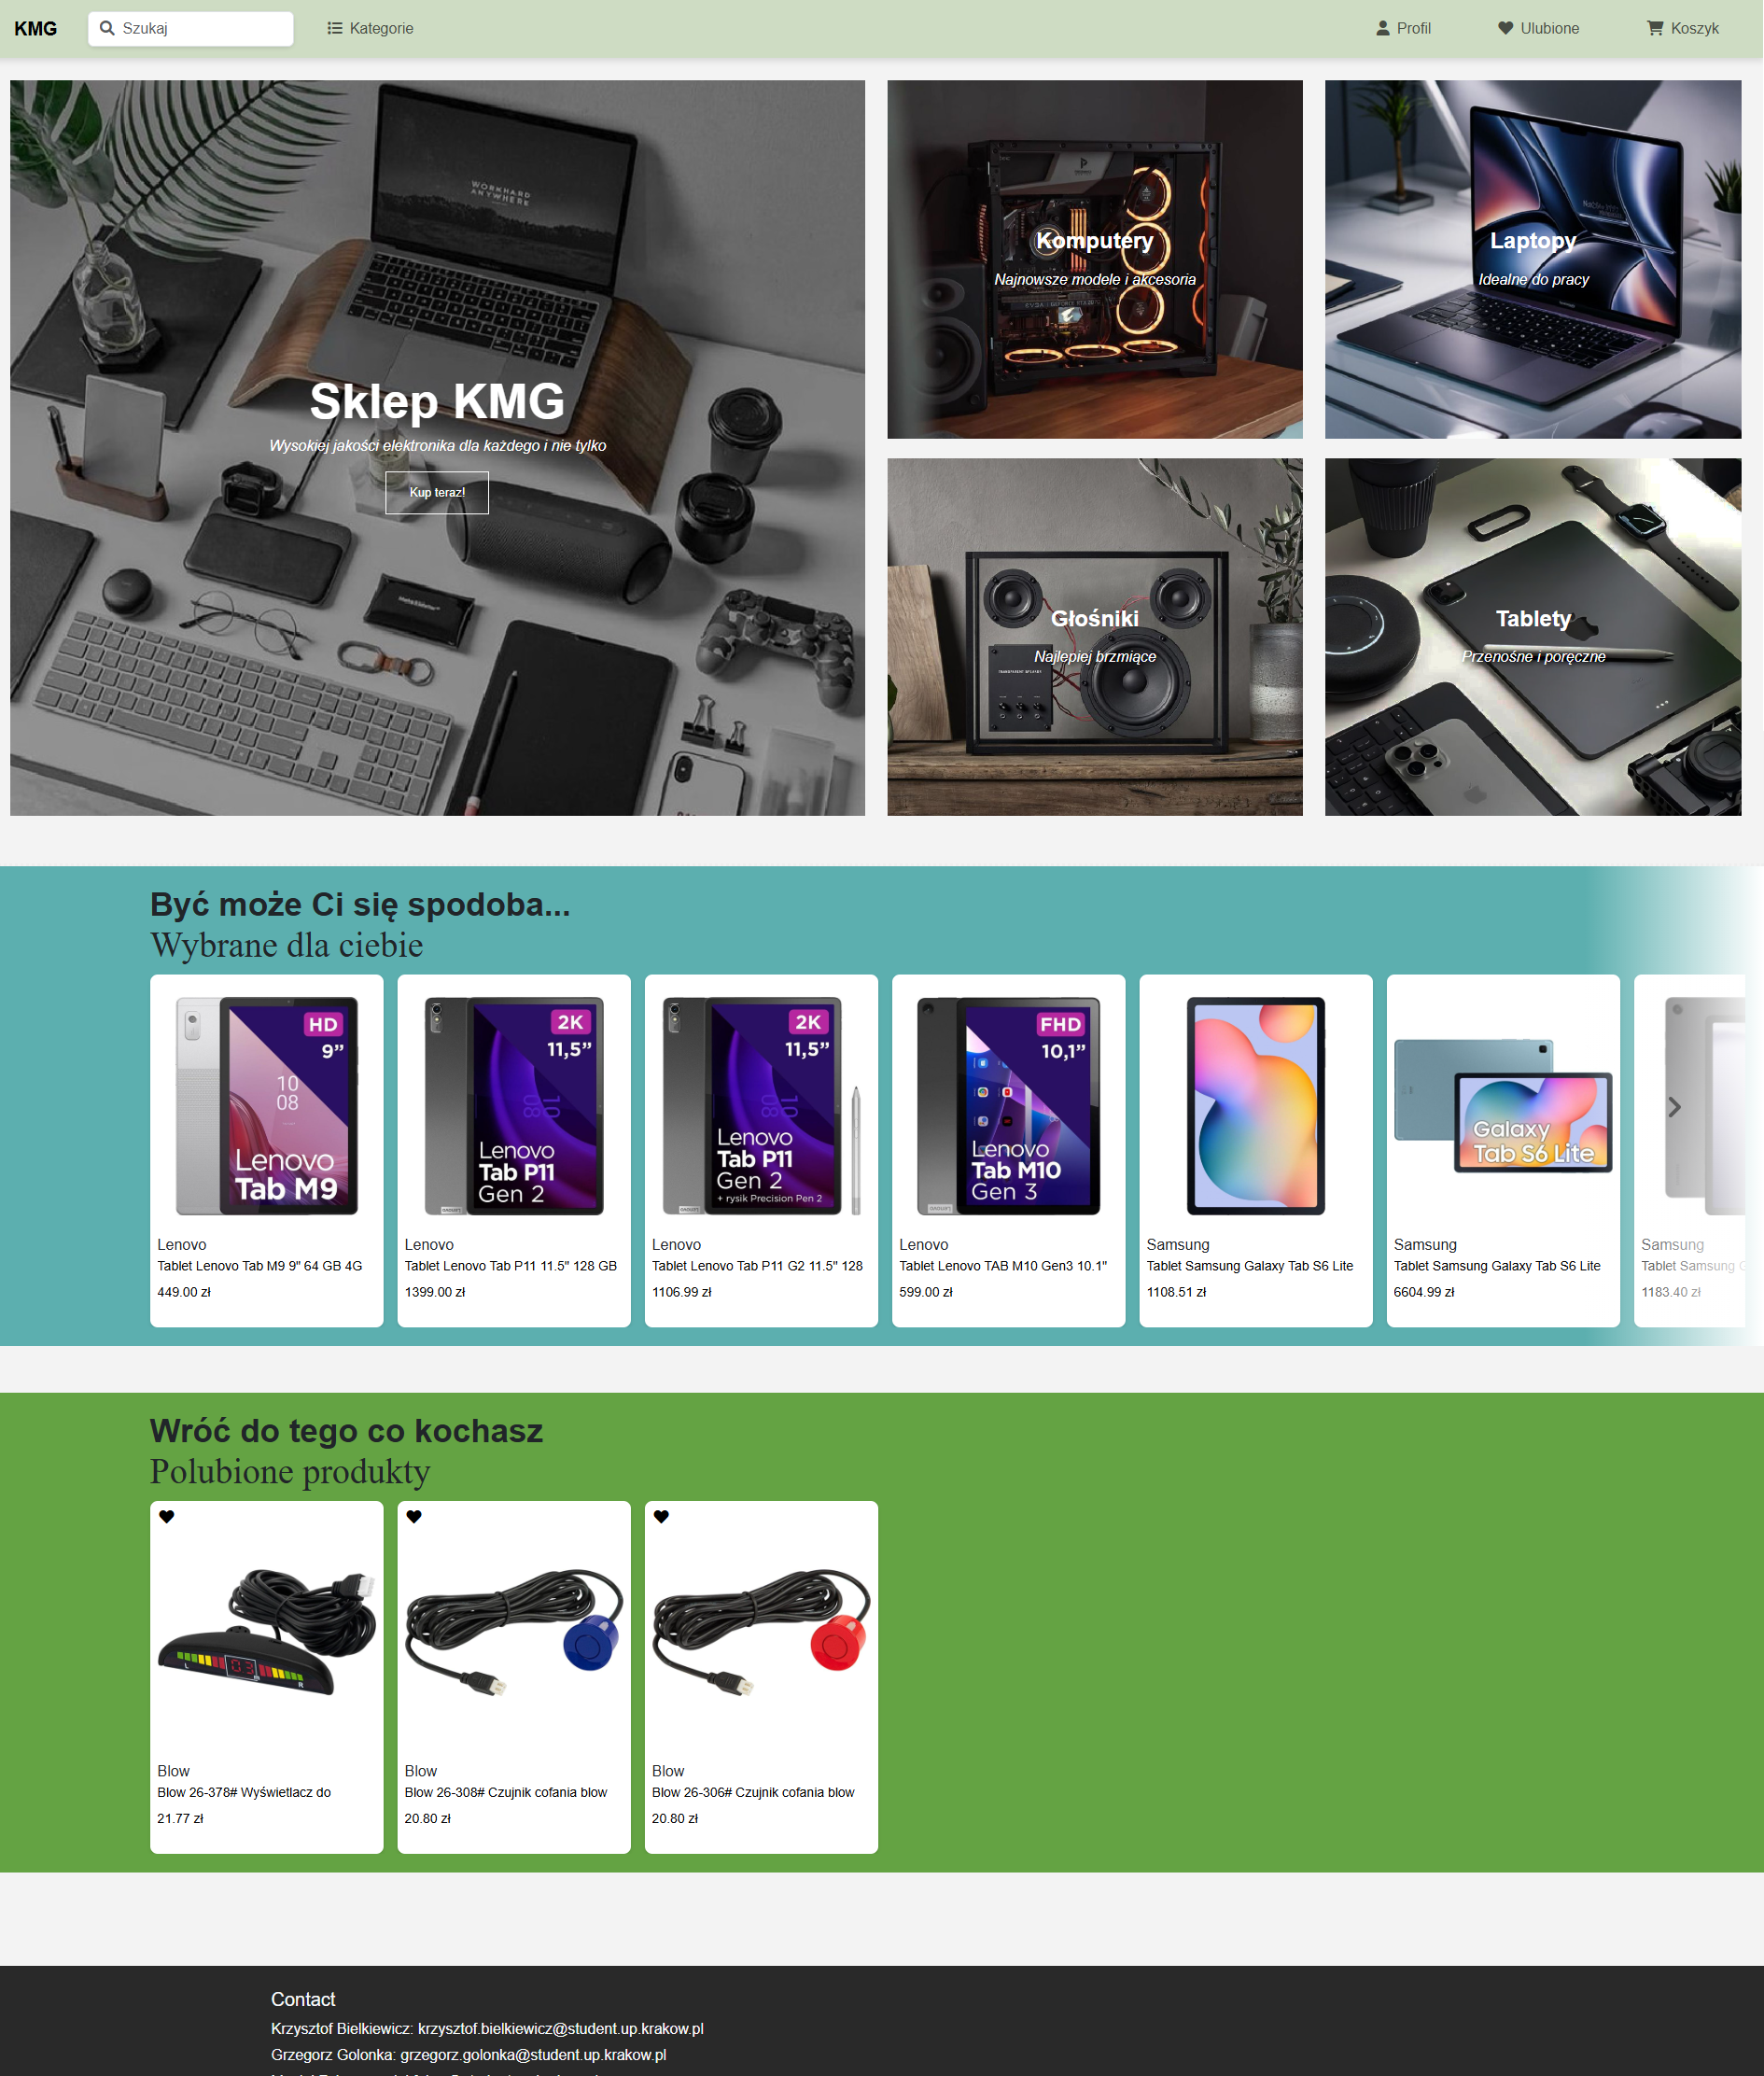
\includegraphics[width=1.0\columnwidth]{screens/main_page.png}
    \caption{Strona główna sklepu internetowego. \emph{Źródło: opracowanie własne.}}
    \label{fig:home_page}
\end{figure}






\newpage
\subsubsection{Wyświetlanie produktów}
System umożliwia przeglądanie dostępnych produktów w sklepie internetowym. Produkty są prezentowane w formie listy zawierającej:
\begin{itemize}
    \item producenta produktu,
    \item nazwę produktu,
    \item cenę,
    \item miniaturkę zdjęcia produktu.
\end{itemize}

\begin{figure}[H]
    \centering
    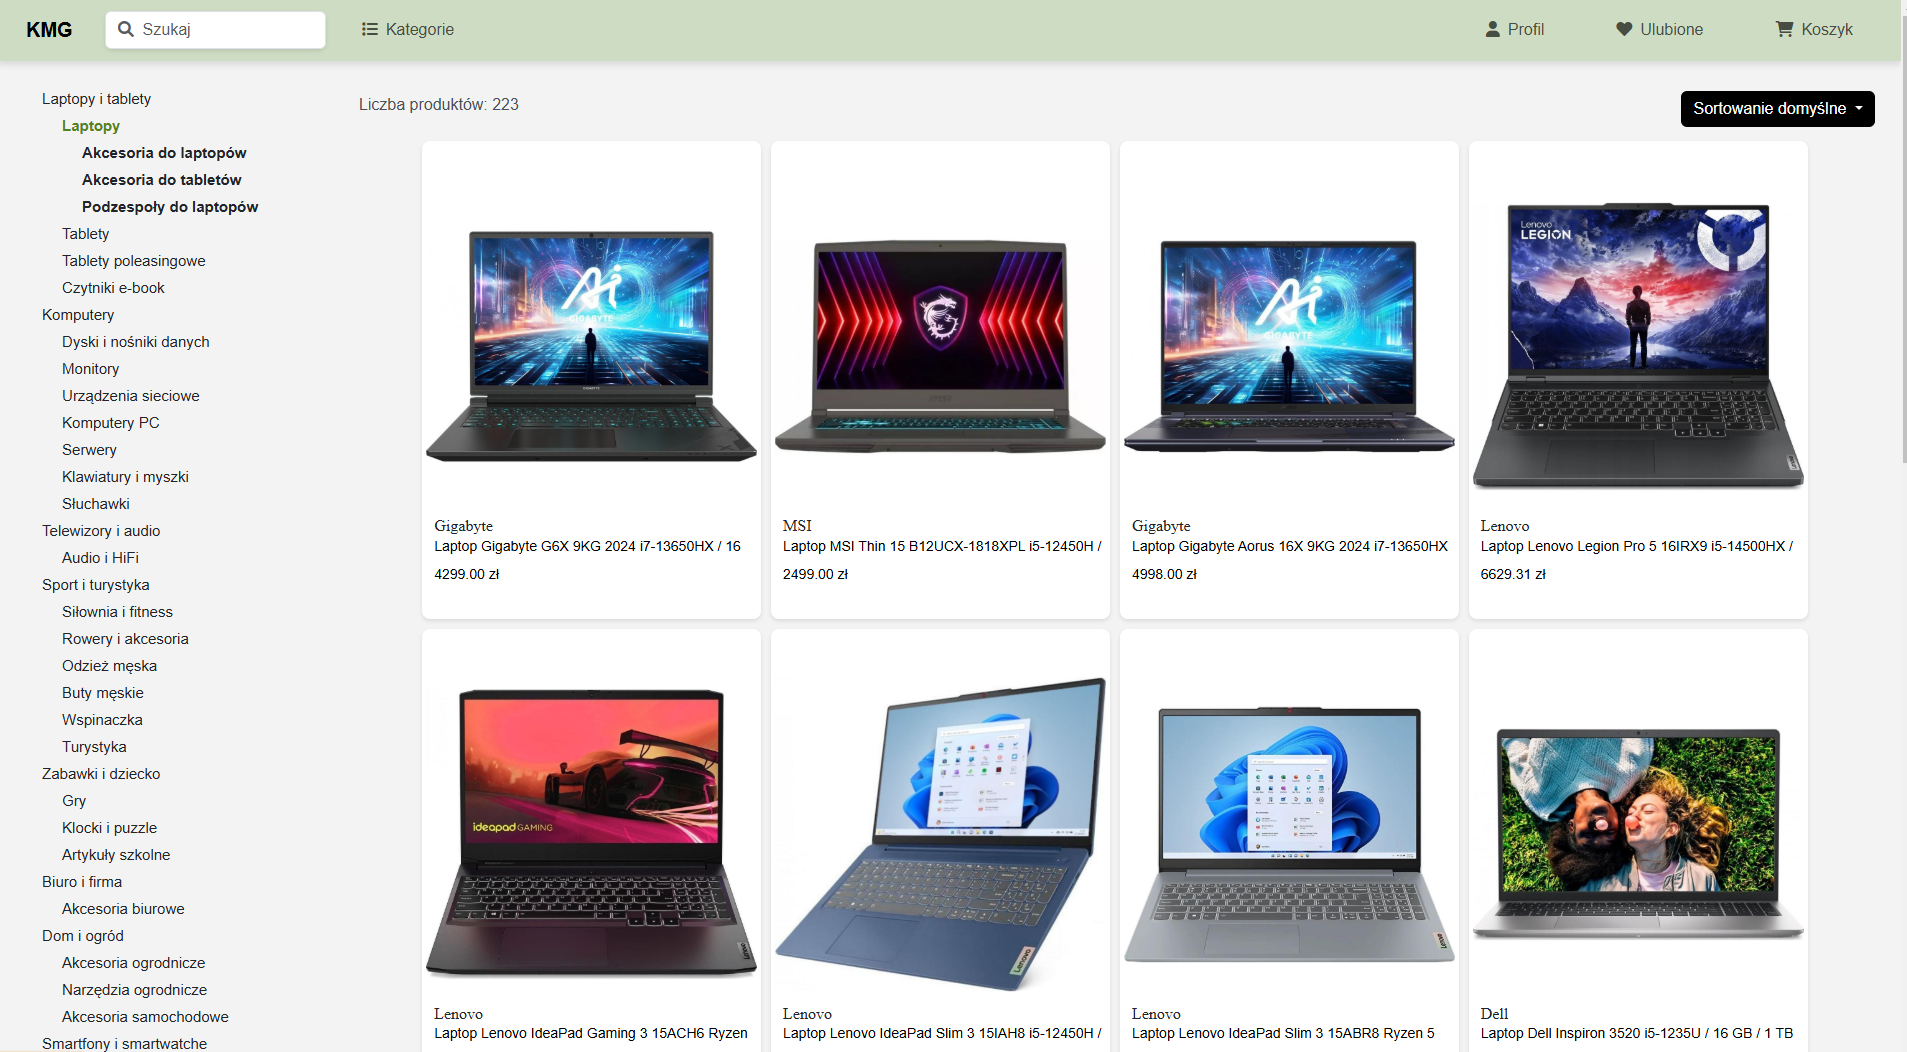
\includegraphics[width=1.0\columnwidth]{screens/products_list.png}
    \caption{Widok listy produktów. \emph{Źródło: opracowanie własne.}}
    \label{fig:product_list}
\end{figure}






\subsubsection{Wyświetlanie kategorii}
Produkty są pogrupowane w kategorie, co pozwala na łatwiejsze przeglądanie zasobów sklepu. Użytkownik ma dwie możliwości wyświetlania kategorii:

\paragraph{Wyświetlanie kategorii przez przycisk w górnym pasku}
Na stronie głównej znajduje się przycisk wyświetlenia kategorii w górnym pasku nawigacyjnym. Po jego kliknięciu użytkownikowi wyświetla się lista dostępnych kategorii, np. takich jak:
\begin{itemize}
    \item Komputery,
    \item Laptopy i tablety,
    \item Telewizory i audio,
    \item Dom i ogród.
\end{itemize}
Każda kategoria zawiera nazwę i podległe jej subkategorie. Po wybraniu kategorii użytkownik zostaje przekierowany do widoku produktów w danej kategorii.

\begin{figure}[H]
    \centering
    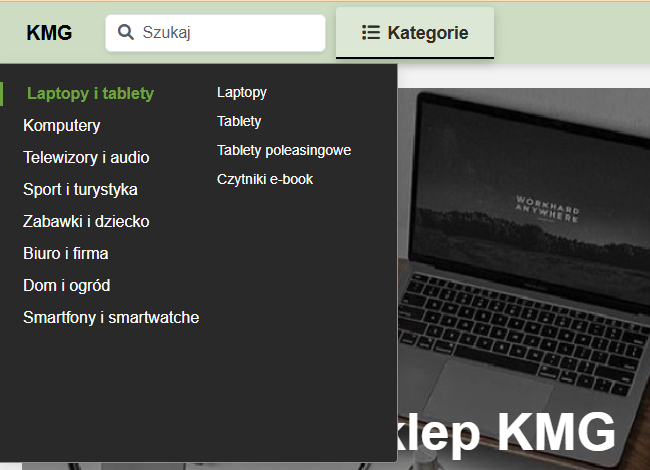
\includegraphics[width=1.0\columnwidth]{screens/categories.png}
    \caption{Widok listy kategorii na górnym pasku. \emph{Źródło: opracowanie własne.}}
    \label{fig:categories_bar}
\end{figure}

\paragraph{Wyświetlanie kategorii w widoku produktów}
Alternatywnie, użytkownik może skorzystać z menu bocznego w widoku produktów. Menu to wyświetla listę kategorii, umożliwiając szybkie przełączanie między kategoriami podczas przeglądania produktów. Lista kategorii w menu bocznym zawiera nazwy kategorii i podkategorii, co umożliwia bardziej precyzyjne filtrowanie.

\begin{figure}[H]
    \centering
    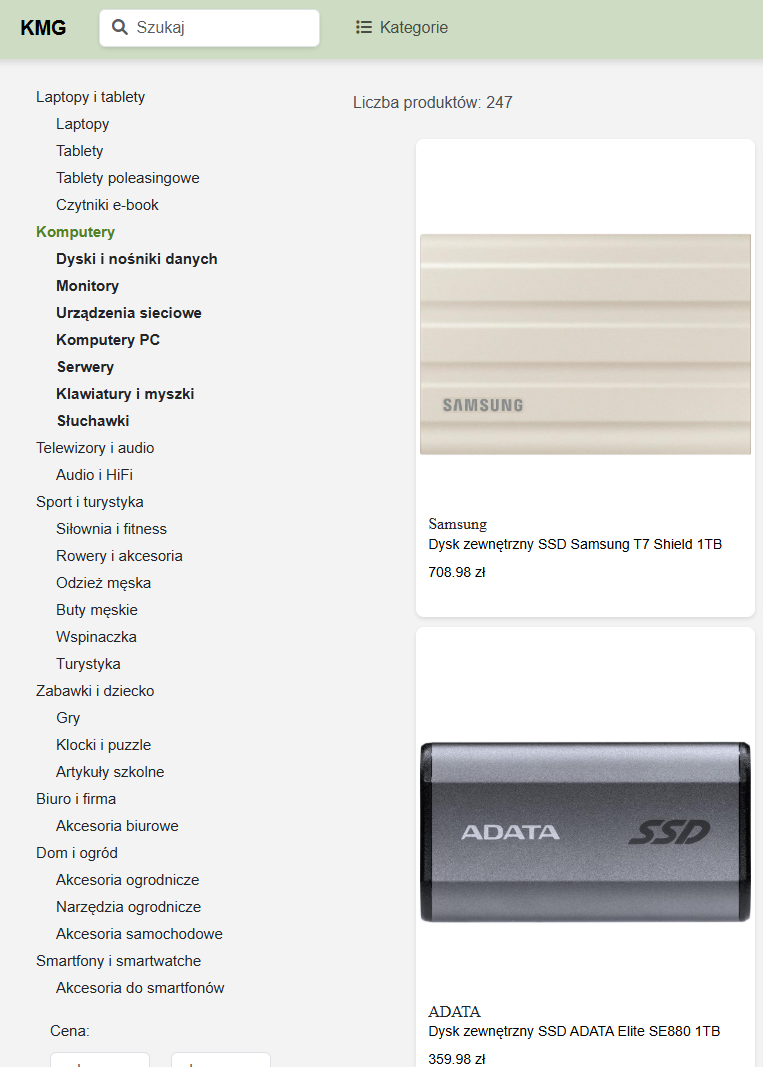
\includegraphics[width=1.0\columnwidth]{screens/categories_products.png}
    \caption{Widok listy kategorii podczas wyświetlania produktów. \emph{Źródło: opracowanie własne.}}
    \label{fig:categories}
\end{figure}






\newpage
\subsubsection{Wyszukiwanie produktów}
System posiada funkcję wyszukiwania produktów, co pozwala użytkownikom na szybkie znalezienie interesującego produktu na podstawie wprowadzonego tekstu.
\begin{itemize}
    \item Pole wyszukiwania jest dostępne na każdej podstronie serwisu.
    \item Wyniki wyszukiwania są prezentowane w formie listy podobnej do widoku ogólnego produktów.
\end{itemize}

\begin{figure}[H]
    \centering
    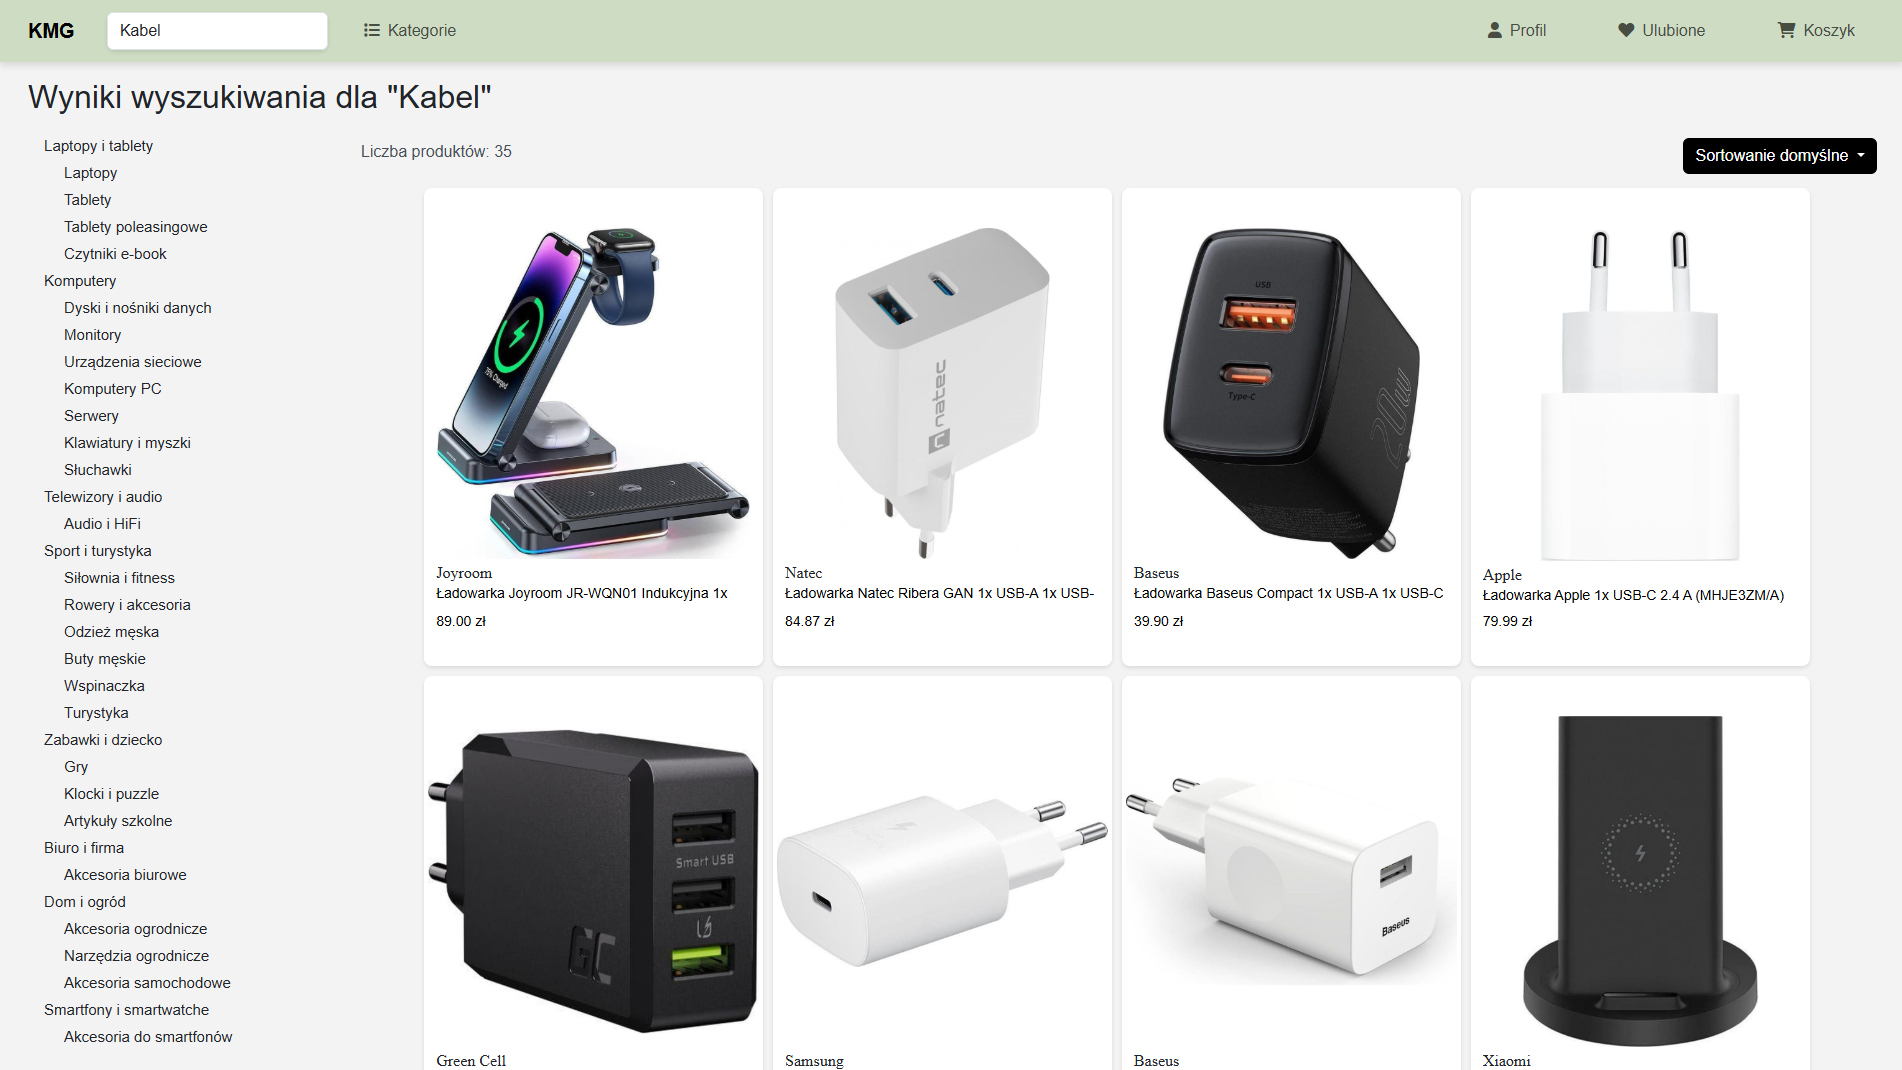
\includegraphics[width=1.0\columnwidth]{screens/search_result.png}
    \caption{Widok wyszukanych produktów dla podanego słowa kluczowego. \emph{Źródło: opracowanie własne.}}
    \label{fig:search_products}
\end{figure}






\newpage
\subsubsection{Lajkowanie produktów}
Użytkownicy mogą polubić produkty, aby wyrazić swoje zainteresowanie lub zapamiętać produkty do przyszłych zakupów. Lajkowanie produktów może odbywać się na dwa sposoby:

\paragraph{Lajkowanie przez miniaturę produktu}
W widoku listy produktów, obok każdej miniatury produktu, znajduje się przycisk „Lubię to”. Kliknięcie tego przycisku oznacza produkt jako ulubiony. Użytkownik może również cofnąć lajka, klikając ponownie ten sam przycisk.

\begin{figure}[H]
    \centering
    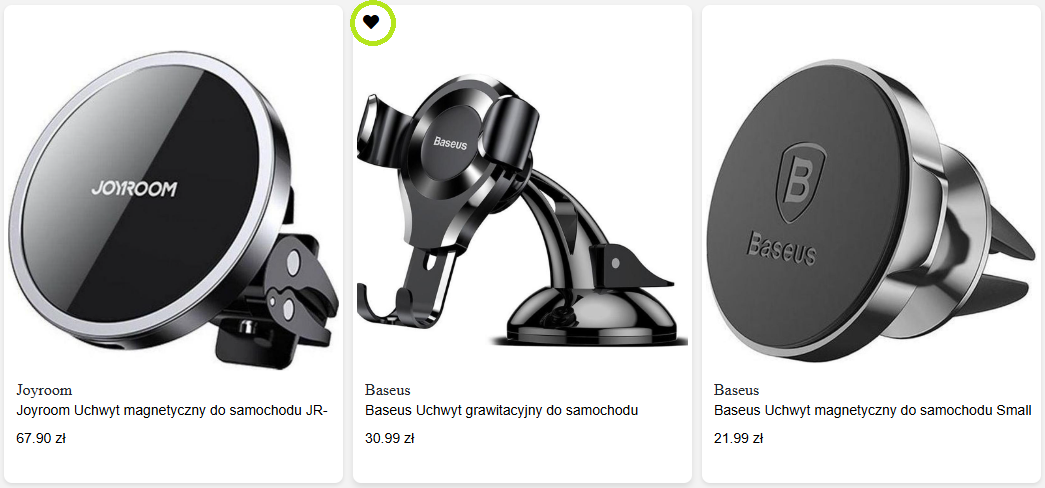
\includegraphics[width=1.0\columnwidth]{screens/like_product_products.png}
    \caption{Miniatura produktu z aktywnym przyciskiem „Lubię to”. \emph{Źródło: opracowanie własne.}}
    \label{fig:like_button_miniature}
\end{figure}

\paragraph{Lajkowanie w szczegółach produktu}
Alternatywnie, użytkownik może polubić produkt w widoku szczegółowym. Przycisk „Lubię to” znajduje się w widocznym miejscu obok przycisku "Dodaj do koszyka". Ten sposób jest szczególnie przydatny, gdy użytkownik chce zapoznać się z dokładniejszymi informacjami przed polubieniem.
\begin{figure}[H]
    \centering
    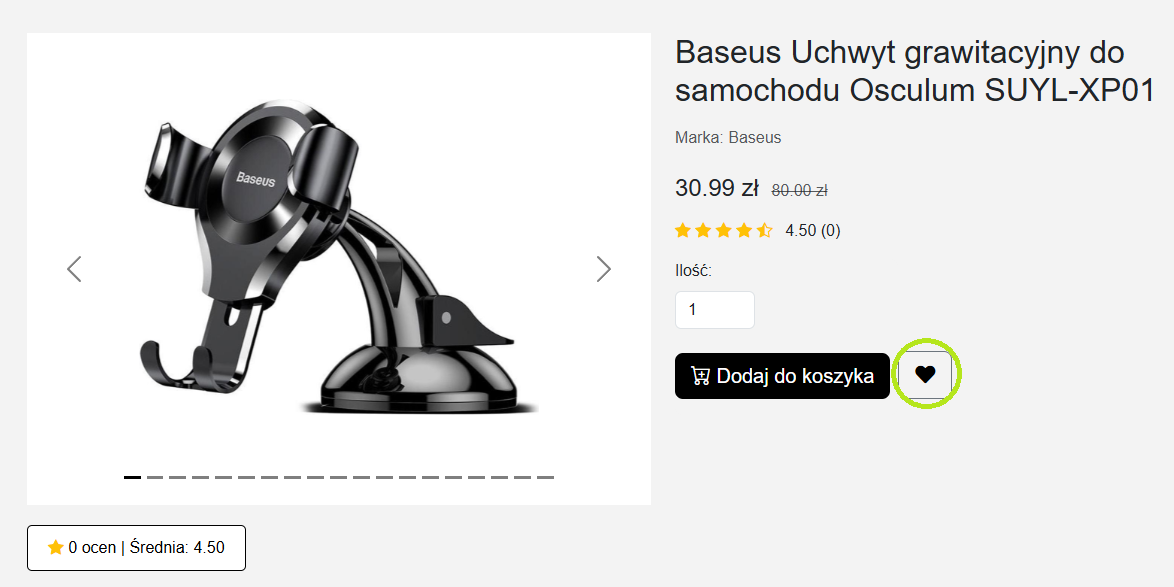
\includegraphics[width=1.0\columnwidth]{screens/like_product_details.png}
    \caption{Produkt z aktywnym przyciskiem „Lubię to”. \emph{Źródło: opracowanie własne.}}
    \label{fig:like_button_details}
\end{figure}
\begin{itemize}
    \item Lajki są zapisywane w bazie danych użytkownika (dla zalogowanych użytkowników) lub w sesji przeglądarki (dla użytkowników niezalogowanych).
    \item Produkty oznaczone jako ulubione są widoczne w sekcji ulubionych produktów.
    \begin{figure}[H]
        \centering
        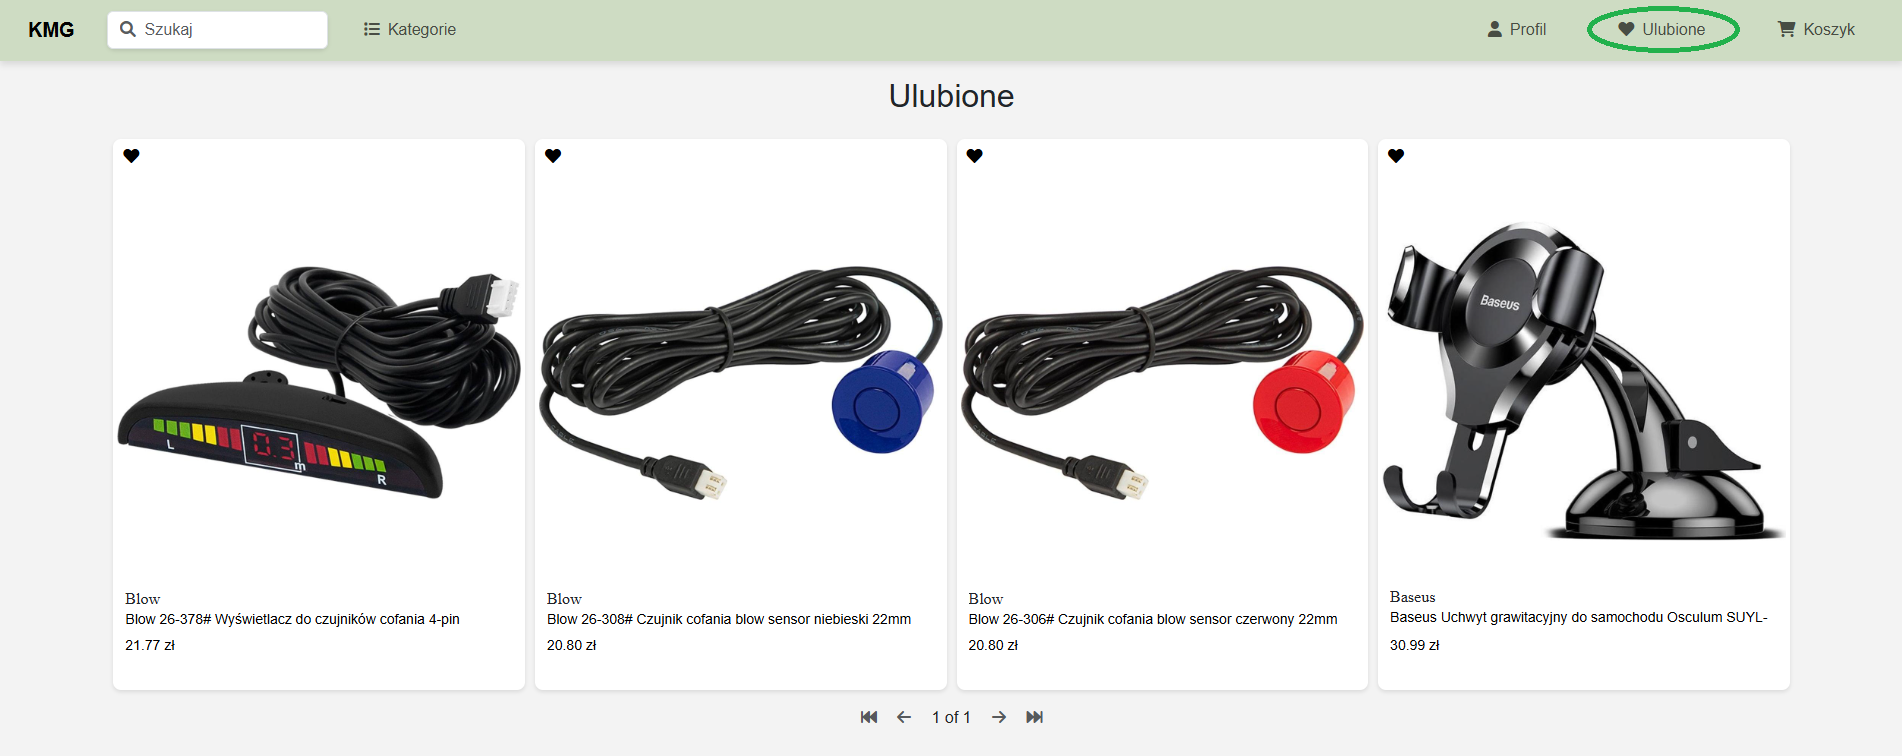
\includegraphics[width=1.0\columnwidth]{screens/liked_products.png}
        \caption{Polubione produkty (zaznaczony przycisk wyświetlający polubione produkty). \emph{Źródło: opracowanie własne.}}
        \label{fig:liked_products}
    \end{figure}
\end{itemize}







\newpage
\subsubsection{Wyświetlanie szczegółów produktu}
Widok szczegółowy produktu zawiera:
\begin{itemize}
    \item nazwę produktu,
    \item cenę,
    \item szczegółowy opis produktu,
    \item pełnowymiarowe zdjęcia produktu,
    \item ocenę oraz przyciski do lajkowania i zakupu produktu,
    \item pole wyboru ilości produktu, który zostanie dodany do koszyka.
\end{itemize}

\paragraph{Pole wyboru ilości produktu}
W widoku szczegółowym produktu znajduje się pole wejściowe (input), które pozwala użytkownikowi określić ilość produktu do dodania do koszyka. Domyślnie ilość jest ustawiona na 1, ale użytkownik może ją zmienić, wpisując inną wartość lub korzystając z przycisków zwiększania/zmniejszania ilości.

\begin{itemize}
    \item Pole obsługuje tylko liczby dodatnie.
    \item Jeśli użytkownik wprowadzi wartość ujemną lub zerową, system wyświetli stosowny komunikat o błędzie.
\end{itemize}

\begin{figure}[H]
    \centering
    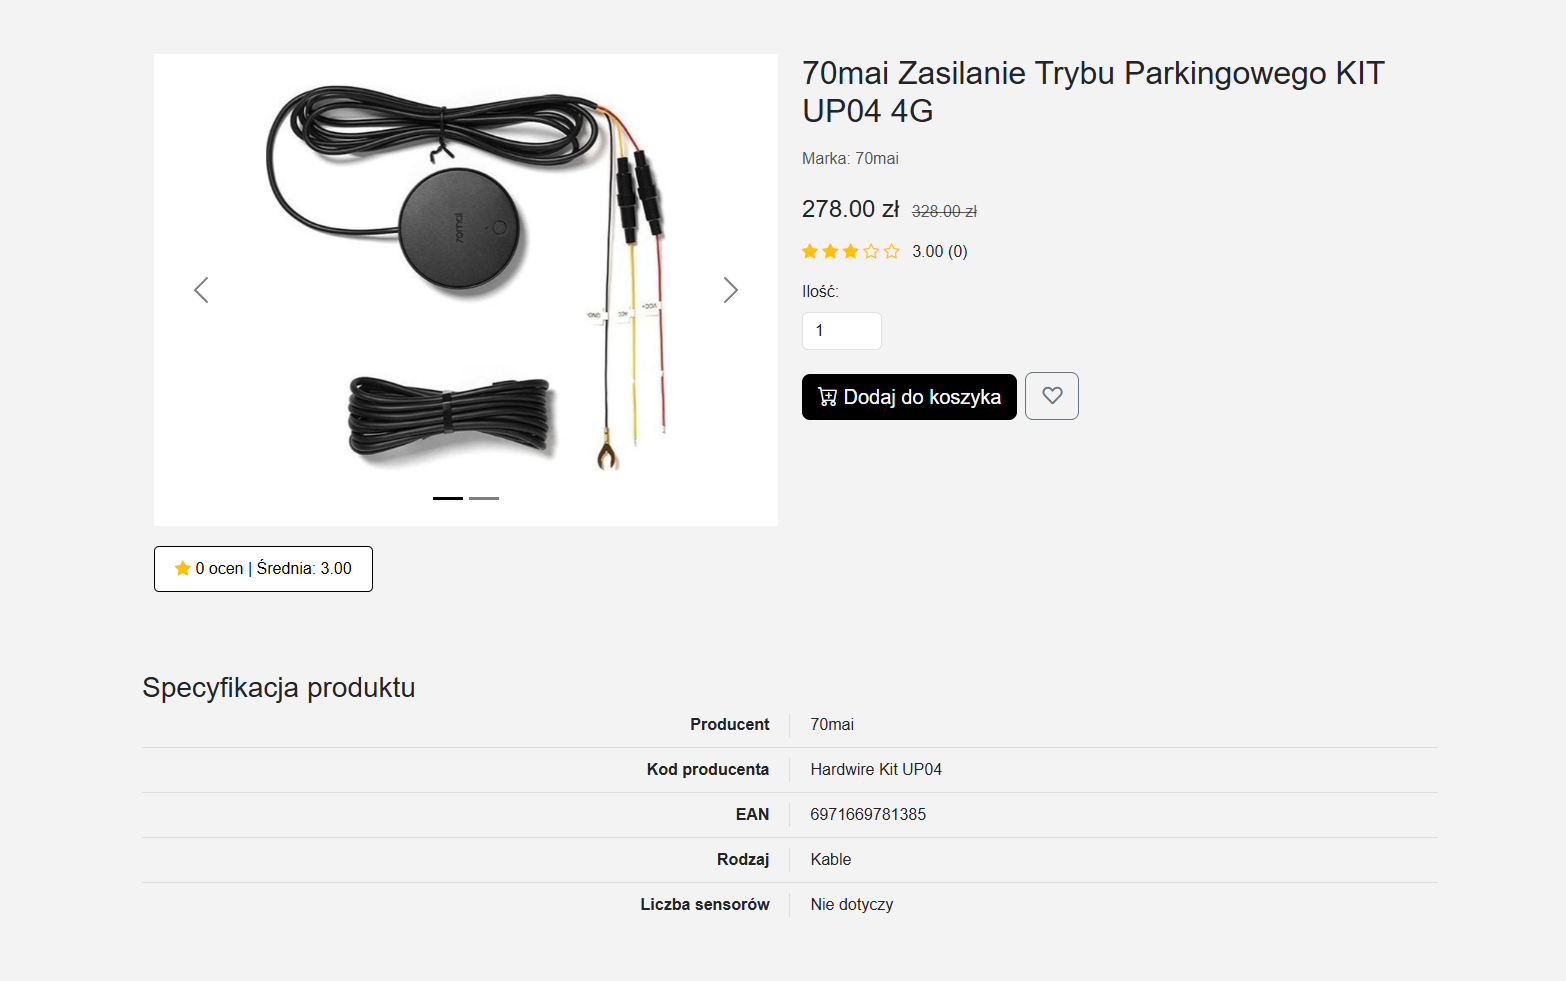
\includegraphics[width=1.0\columnwidth]{screens/product_details.png}
    \caption{Widok szczegółowy produktu z polem wyboru ilości. \emph{Źródło: opracowanie własne.}}
    \label{fig:product_details}
\end{figure}







\newpage
\subsubsection{Wyświetlanie ocen produktów}
Każdy produkt posiada ocenę, która jest średnią ocen użytkowników. Szczegółowy widok produktu zawiera przycisk wyświetlający dodatkowe informacje o ocenach i opiniach.

\paragraph{Prezentacja średniej oceny i liczby ocen}
W widoku szczegółowym produktu znajduje się przycisk, na którym wyświetlana jest średnia ocena produktu (w skali od 1 do 5) oraz liczba wszystkich ocen. Przycisk ten umożliwia przejście do widoku opinii o produkcie.

\begin{figure}[H]
    \centering
    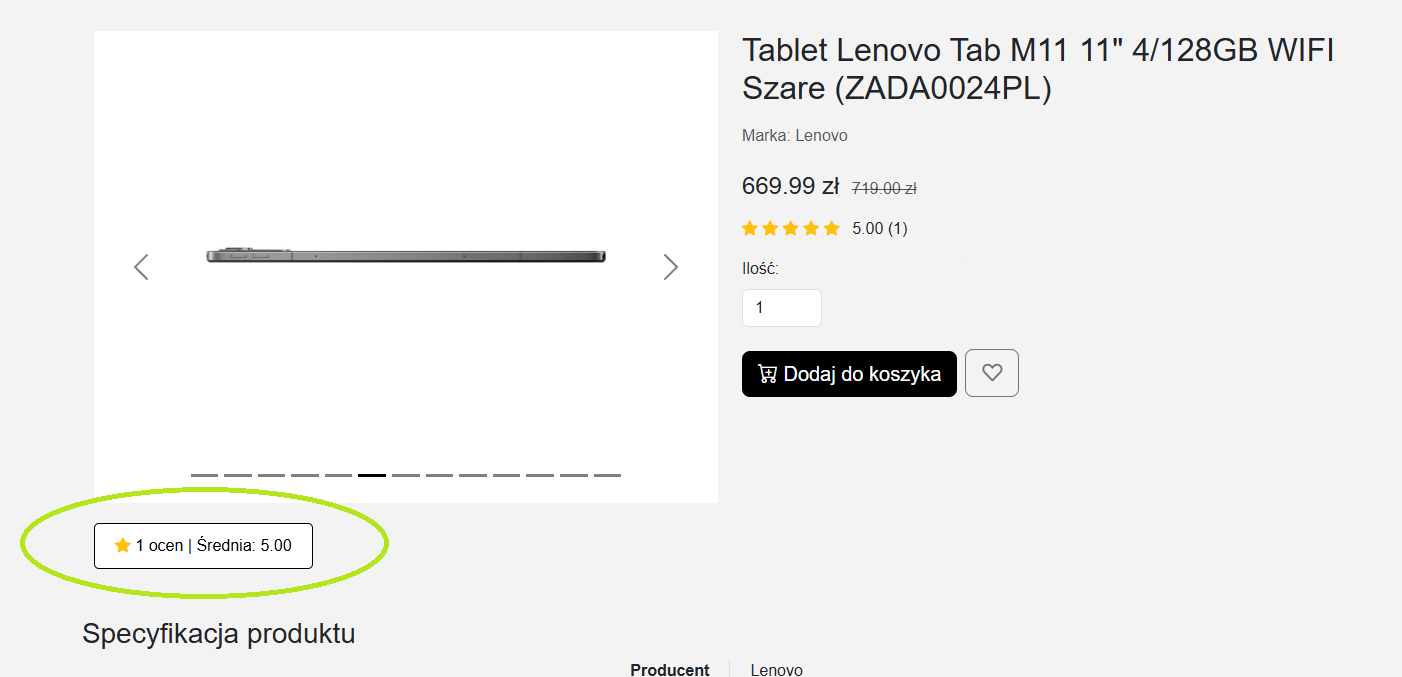
\includegraphics[width=1.0\columnwidth]{screens/opinion_button.png}
    \caption{Przycisk wyświetlający średnią ocenę i liczbę ocen. \emph{Źródło: opracowanie własne.}}
    \label{fig:rating_button}
\end{figure}

\paragraph{Widok opinii o produkcie}
Po kliknięciu przycisku z ocenami użytkownik zostaje przeniesiony do widoku opinii o produkcie. Widok ten zawiera:
\begin{itemize}
    \item Listę wszystkich opinii o produkcie, jeśli takie istnieją:
    \begin{itemize}
        \item Nazwę użytkownika, który dodał opinię,
        \item Treść opinii,
        \item Datę oraz godzinę dodania opinii.
    \end{itemize}
    \begin{figure}[H]
        \centering
        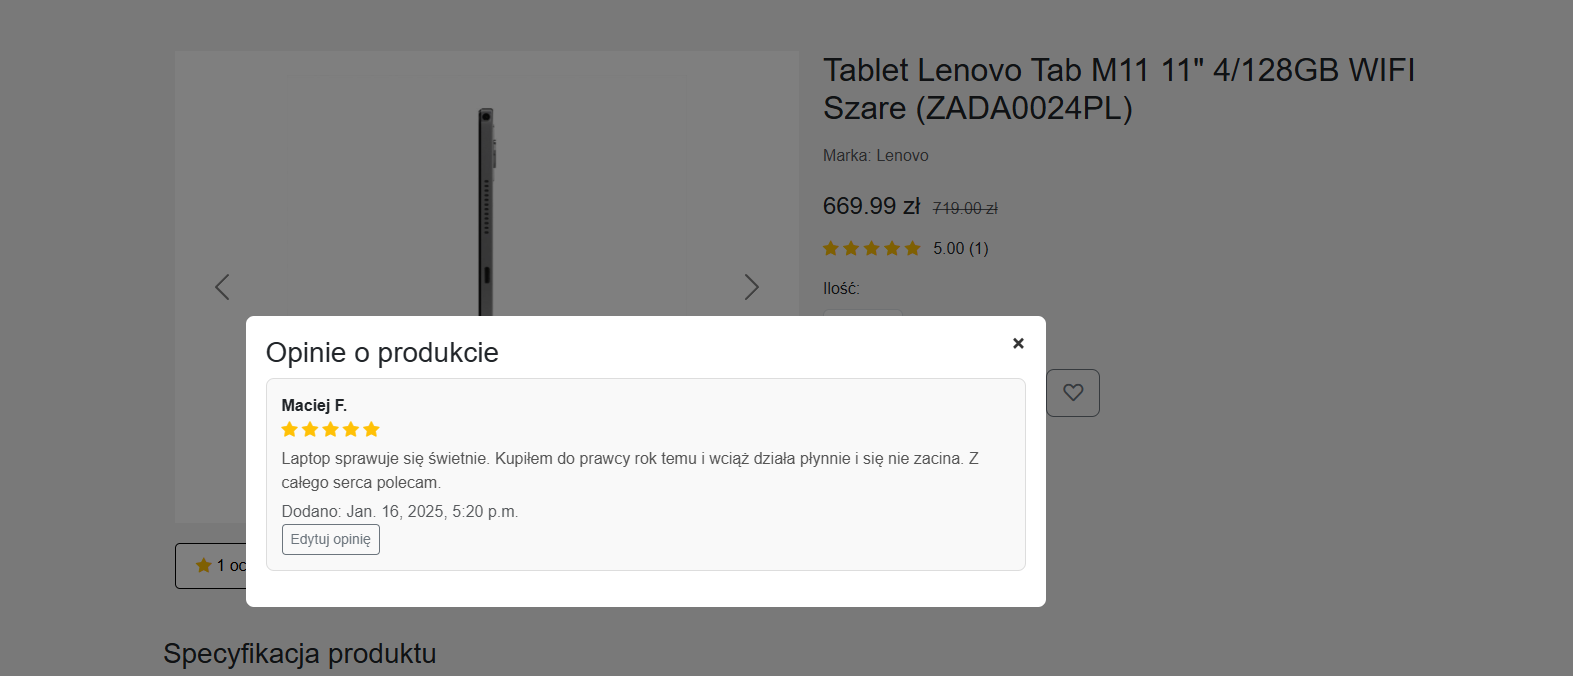
\includegraphics[width=1.0\columnwidth]{screens/product_with_opinion.png}
        \caption{Widok opinii o produkcie. \emph{Źródło: opracowanie własne.}}
        \label{fig:review_list}
    \end{figure}
    \item Jeśli produkt nie posiada jeszcze opinii, wyświetlana jest informacja o ich braku.
    \begin{figure}[H]
        \centering
        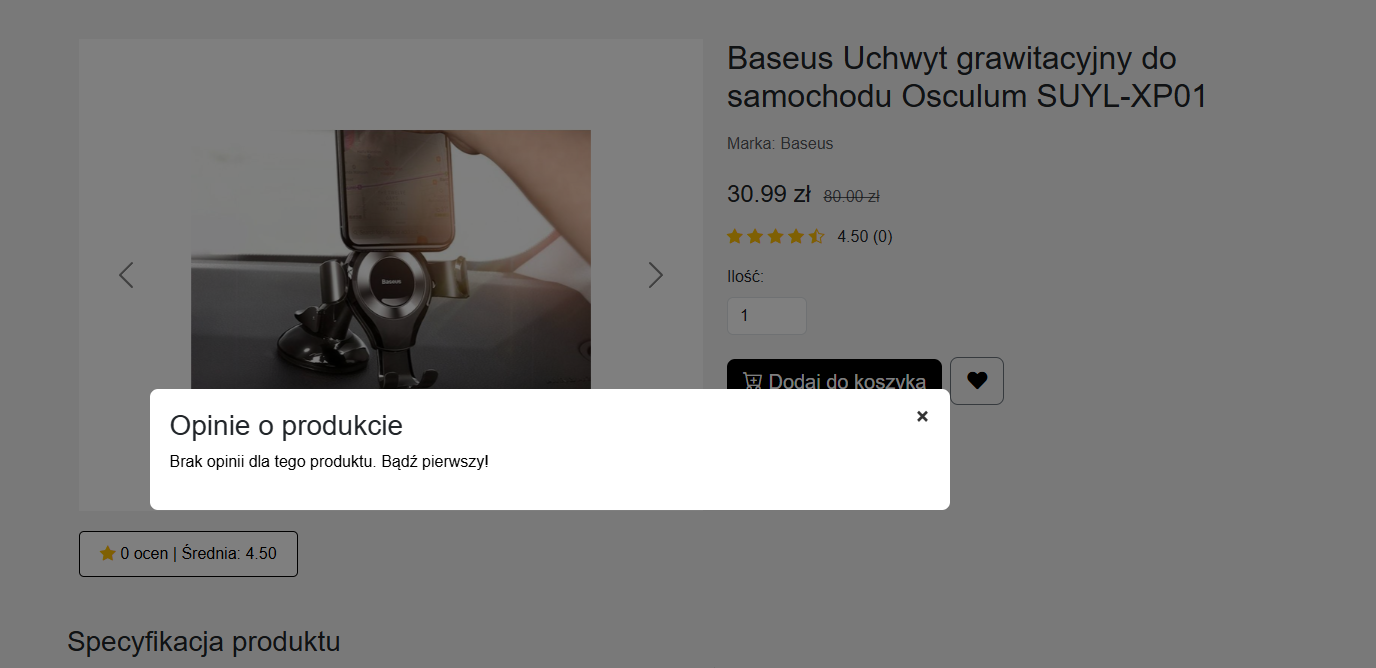
\includegraphics[width=1.0\columnwidth]{screens/product_without_opinions.png}
        \caption{Informacja o braku opinii o produkcie. \emph{Źródło: opracowanie własne.}}
        \label{fig:no_reviews}
    \end{figure}
    
\end{itemize}






\subsubsection{Rejestracja użytkownika}
Proces rejestracji umożliwia użytkownikom tworzenie kont w sklepie internetowym, co pozwala na pełne korzystanie z funkcjonalności, takich jak dodawanie produktów do koszyka, przeglądanie historii zakupów czy tworzenie opinii.

\paragraph{Formularz rejestracji}
Rejestracja odbywa się poprzez formularz dostępny na stronie rejestracji. Formularz wymaga od użytkownika podania następujących informacji:
\begin{itemize}
    \item Imię,
    \item Nazwisko,
    \item Adres e-mail – używany jako login,
    \item Numer telefonu,
    \item Data urodzenia,
    \item Płeć,
    \item Hasło – musi spełniać kryteria bezpieczeństwa, takie jak minimalna długość (np. 8 znaków) oraz zawartość (przynajmniej jedna duża litera, jedna cyfra itp.),
\end{itemize}

\begin{figure}[H]
    \centering
    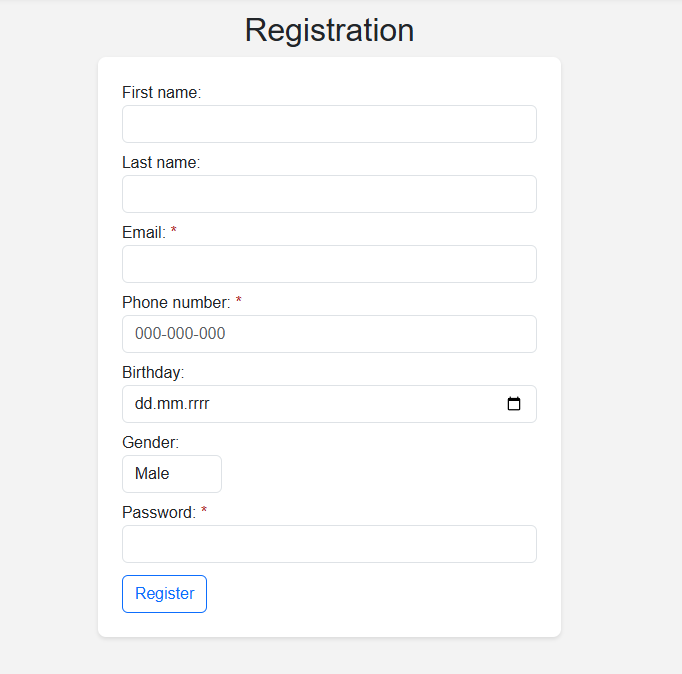
\includegraphics[width=1.0\columnwidth]{screens/register_form.png}
    \caption{Formularz rejestracji. \emph{Źródło: opracowanie własne.}}
    \label{fig:registration_form}
\end{figure}

\paragraph{Proces rejestracji}
1. Użytkownik wypełnia formularz i klika przycisk „Zarejestruj się”. \newline
2. System sprawdza poprawność wprowadzonych danych:
   \begin{itemize}
       \item Jeśli dane są poprawne, konto zostaje utworzone, a użytkownik otrzymuje e-mail potwierdzenie rejestracji.
       \item Jeśli dane są niepoprawne (np. adres email był już użyty do rejestracji), system wyświetla odpowiednie komunikaty o błędach.
       \begin{figure}[H]
        \centering
        
\includegraphics[width=1.0\columnwidth]{screens/invalid__registration_form.png}
        \caption{Błędny formularz rejestracji. \emph{Źródło: opracowanie własne.}}
        \label{fig:invalid_registration_form}
    \end{figure}
   \end{itemize}

\paragraph{Zabezpieczenia procesu rejestracji}
System rejestracji zawiera następujące zabezpieczenia:
\begin{itemize}
    \item Sprawdzenie unikalności adresu e-mail – użytkownik nie może zarejestrować dwóch kont z tym samym adresem.
    \item Walidacja danych wejściowych – system weryfikuje poprawność formatu e-maila oraz spełnienie wymagań hasła.
    \item Wlidacja imienia, nazwiska, numeru telefonu oraz daty urodzenia.
\end{itemize}







\subsubsection{Logowanie użytkownika}
Logowanie pozwala użytkownikom na dostęp do konta w sklepie internetowym, umożliwiając korzystanie z funkcji personalizacji, takich jak zapisane ulubione produkty, historia zakupów czy możliwość dodawania opinii.

\paragraph{Formularz logowania}
Logowanie odbywa się poprzez formularz dostępny na dedykowanej stronie. Formularz logowania wymaga podania:
\begin{itemize}
    \item Adresu e-mail – używanego jako login,
    \item Hasła – zgodnego z hasłem podanym podczas rejestracji.
\end{itemize}
\begin{figure}[H]
    \centering
    
\includegraphics[width=1.0\columnwidth]{screens/login_form.png}
    \caption{Formularz logowania użytkownika. \emph{Źródło: opracowanie własne.}}
    \label{fig:login_form}
\end{figure}
\paragraph{Proces logowania}
1. Użytkownik wprowadza adres e-mail oraz hasło w formularzu logowania.\newline
2. Po kliknięciu przycisku „Zaloguj się” system weryfikuje dane:
   \begin{itemize}
       \item Jeśli dane są poprawne, użytkownik zostaje zalogowany i przeniesiony na stronę główną z dostępem do funkcji konta.
       \item Jeśli dane są niepoprawne, system wyświetla komunikat o błędzie.
       \begin{figure}[H]
        \centering
        
\includegraphics[width=1.0\columnwidth]{screens/invalid_login_form.png}
        \caption{Błędny formularz logowania użytkownika. \emph{Źródło: opracowanie własne.}}
        \label{fig:invalid_login_form}
    \end{figure}
   \end{itemize}






\newpage
   \subsubsection{Dodawanie produktów do koszyka}
   Użytkownicy mogą dodawać produkty do koszyka zarówno z widoku miniatury produktu, jak i z widoku szczegółowego. Koszyk umożliwia zapisywanie produktów zarówno dla zalogowanych użytkowników, jak i w sesji dla użytkowników niezalogowanych.
   
   \paragraph{Dodawanie produktów z miniatury produktu}
   W widoku listy produktów, obok każdej miniatury, znajduje się przycisk w kształcie koszyka. Kliknięcie tego przycisku powoduje dodanie jednego egzemplarza produktu do koszyka. Pomyślne dodanie produktu spowoduje przeniesienie użytkownika do zawartości całego koszyka.
      
   \begin{figure}[H]
    \centering
    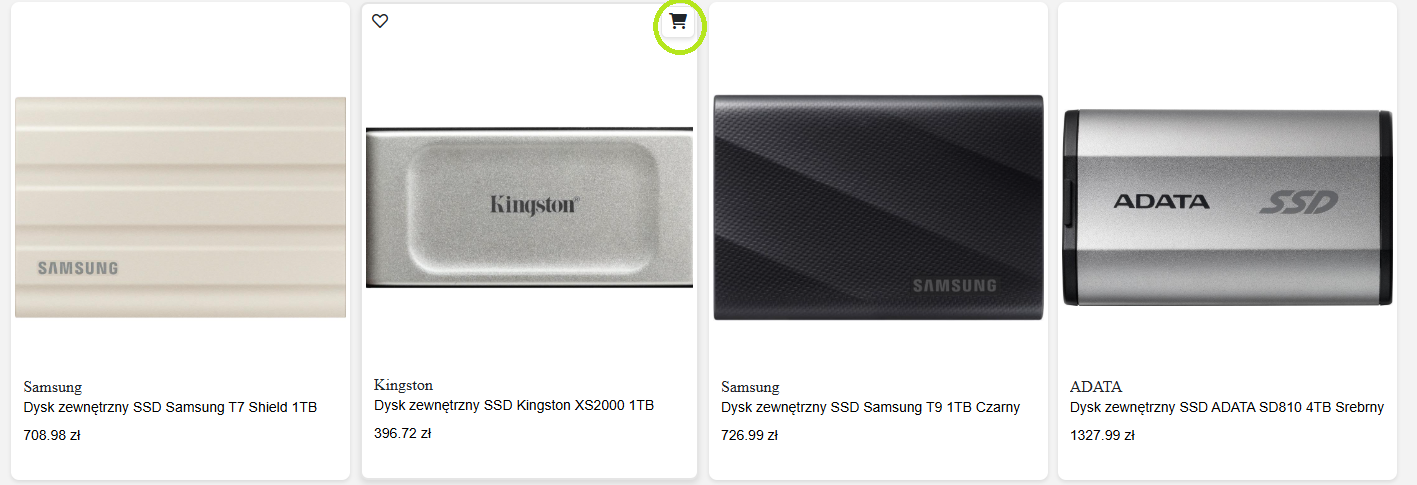
\includegraphics[width=1.0\columnwidth]{screens/add_to_cart_item.png}
    \caption{Dodawanie produktu do koszyka z miniatury. \emph{Źródło: opracowanie własne.}}
    \label{fig:add_to_cart_miniature}
\end{figure}

   \paragraph{Dodawanie produktów w szczegółach produktu}
   W widoku szczegółowym produktu użytkownik może ustawić, ile sztuk produktu chce dodać do koszyka. W tym celu dostępne jest pole wejściowe (input) obok przycisku „Dodaj do koszyka”. Po wprowadzeniu żądanej liczby i kliknięciu przycisku wybrana ilość produktu zostaje dodana do koszyka.
   \begin{figure}[H]
    \centering
    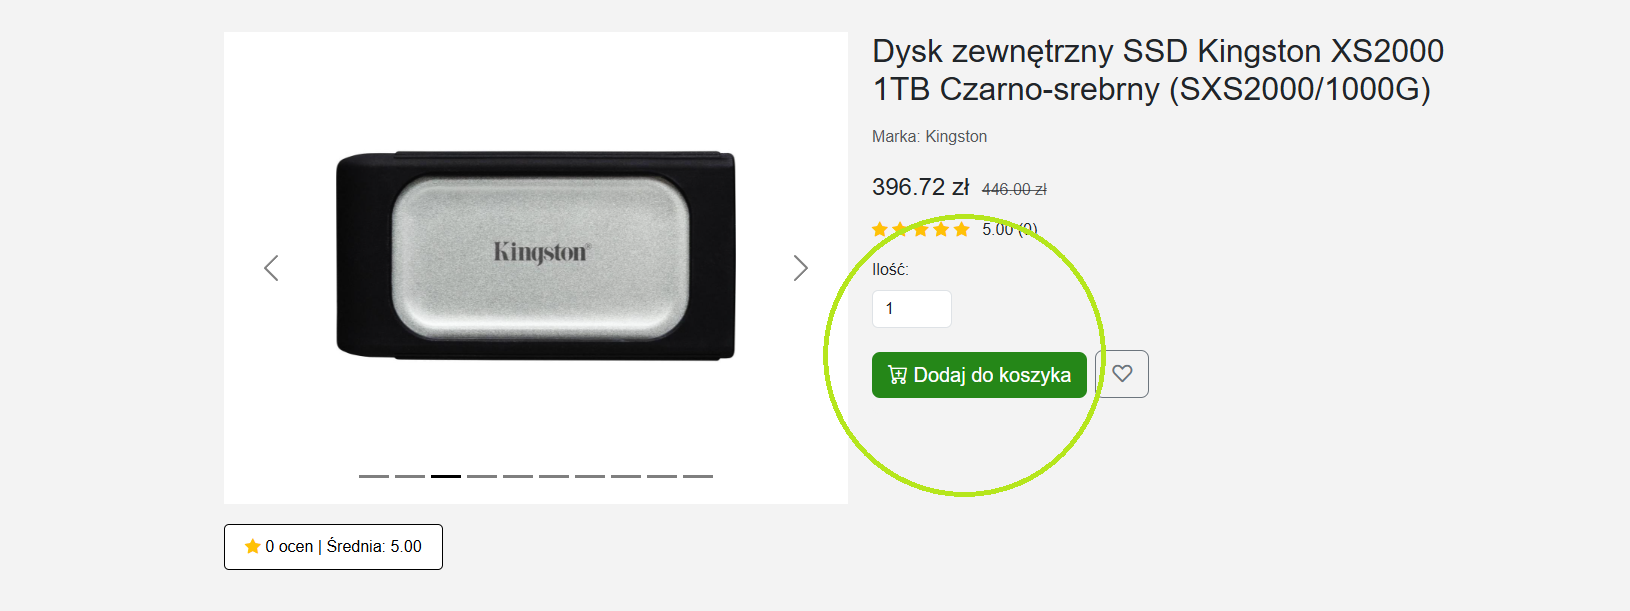
\includegraphics[width=1.0\columnwidth]{screens/add_to_cart_details.png}
    \caption{Dodawanie produktu do koszyka w szczegółach produktu. \emph{Źródło: opracowanie własne.}}
    \label{fig:add_to_cart_details}
\end{figure}

   
   \paragraph{Koszyk dla zalogowanych i niezalogowanych użytkowników}
   \begin{itemize}
       \item **Zalogowani użytkownicy**: Koszyk jest powiązany z kontem użytkownika i przechowuje produkty nawet po wylogowaniu i ponownym zalogowaniu.
       \item **Niezalogowani użytkownicy**: Koszyk jest zapisywany w sesji przeglądarki i dostępny do momentu zamknięcia sesji lub zalogowania się. Użytkownik musi się zalogować, aby zrealizować zamówienie.
   \end{itemize}
   




   \subsubsection{Widok koszyka}
Widok koszyka pozwala użytkownikom zarządzać dodanymi produktami przed przejściem do finalizacji zamówienia. Zawiera szczegółowe informacje o produktach w koszyku oraz opcje ich modyfikacji.

\paragraph{Elementy widoku koszyka}
Widok koszyka zawiera następujące elementy:
\begin{itemize}
    \item Listę produktów dodanych do koszyka:
    \begin{itemize}
        \item nazwę produktu,
        \item pole do zmiany ilości produktu,
        \item łączną cenę produktu (cena jednostkowa pomnożona przez ilość).
    \end{itemize}
    \item Opcję usunięcia produktu z koszyka – dostępna obok każdego produktu w postaci przycisku „Usuń”.
    \item Całkowitą cenę koszyka – wyświetlaną na dole widoku.
    \item Przycisk „Przejdź do opcji dostawy” – umożliwiający kontynuację procesu zamówienia.
\end{itemize}

\paragraph{Zarządzanie ilością produktów w koszyku}
Użytkownik może zmieniać ilość produktów w koszyku za pomocą pola wejściowego dostępnego przy każdym produkcie:
\begin{itemize}
    \item Wprowadzenie nowej ilości powoduje automatyczną aktualizację łącznej ceny produktu i całkowitej ceny koszyka.
    \item Możliwe jest operowanie tylko na liczbach dodatnich.
\end{itemize}

\paragraph{Usuwanie produktów z koszyka}
Użytkownik może usunąć dowolny produkt z koszyka, klikając przycisk „Usuń” obok produktu. Po usunięciu:
\begin{itemize}
    \item Produkt znika z listy produktów w koszyku,
    \item Całkowita cena koszyka jest automatycznie aktualizowana.
\end{itemize}

\paragraph{Całkowita cena koszyka}
Na dole widoku koszyka wyświetlana jest suma wszystkich produktów w koszyku, uwzględniająca ich ilość i ceny jednostkowe. Cena jest aktualizowana dynamicznie po każdej zmianie ilości lub usunięciu produktu.

\paragraph{Przycisk „Przejdź do opcji dostawy”}
Po zakończeniu zarządzania koszykiem użytkownik może kliknąć przycisk „Przejdź do opcji dostawy”, aby kontynuować proces zamówienia. Ten przycisk przekierowuje do strony, na której można wybrać sposób dostawy i finalizować zamówienie.

\begin{figure}[H]
    \centering
    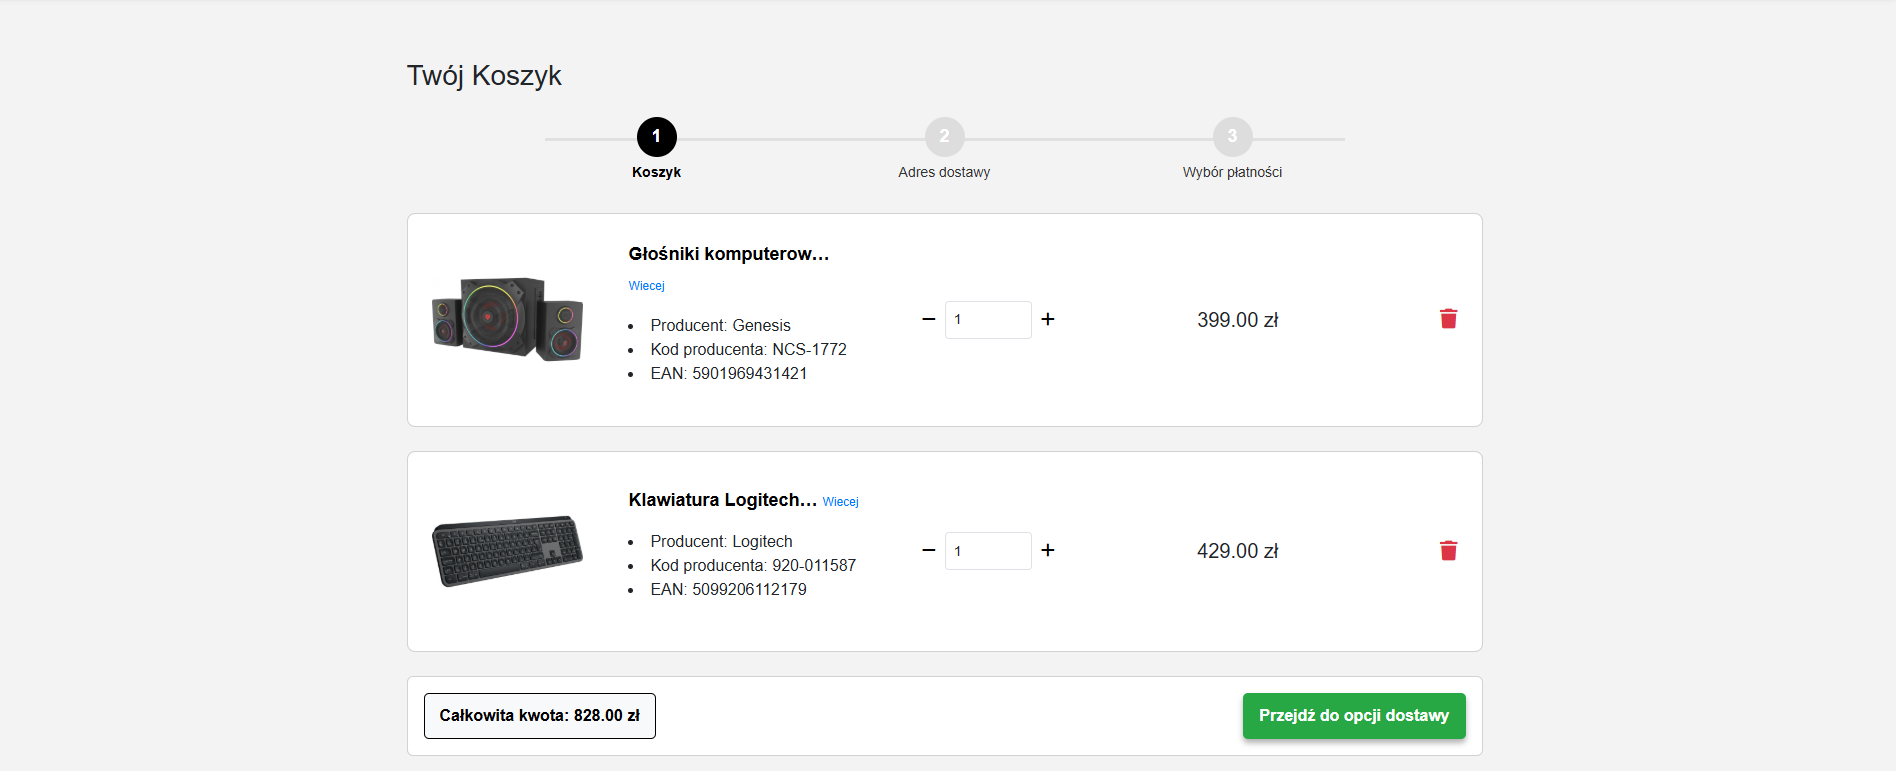
\includegraphics[width=1.0\columnwidth]{screens/cart_view.png}
    \caption{Widok koszyka. \emph{Źródło: opracowanie własne.}}
    \label{fig:cart_view}
\end{figure}





\newpage
\subsubsection{Widok wyboru adresu}
W widoku wyboru adresu użytkownik ma możliwość wskazania adresu dostawy dla zamówienia. Może wybrać jeden z istniejących adresów lub dodać nowy.

\paragraph{Wybór istniejącego adresu}
Jeżeli użytkownik dodał wcześniej adresy, zostaną one wyświetlone w formie listy. Każdy adres zawiera następujące dane:
\begin{itemize}
    \item Ulicę,
    \item Miasto,
    \item Kod pocztowy,
    \item Kraj.
\end{itemize}
Użytkownik może wybrać adres z listy poprzez kliknięcie przycisku „Wybierz” znajdującego się obok danego adresu.
\begin{figure}[H]
    \centering
    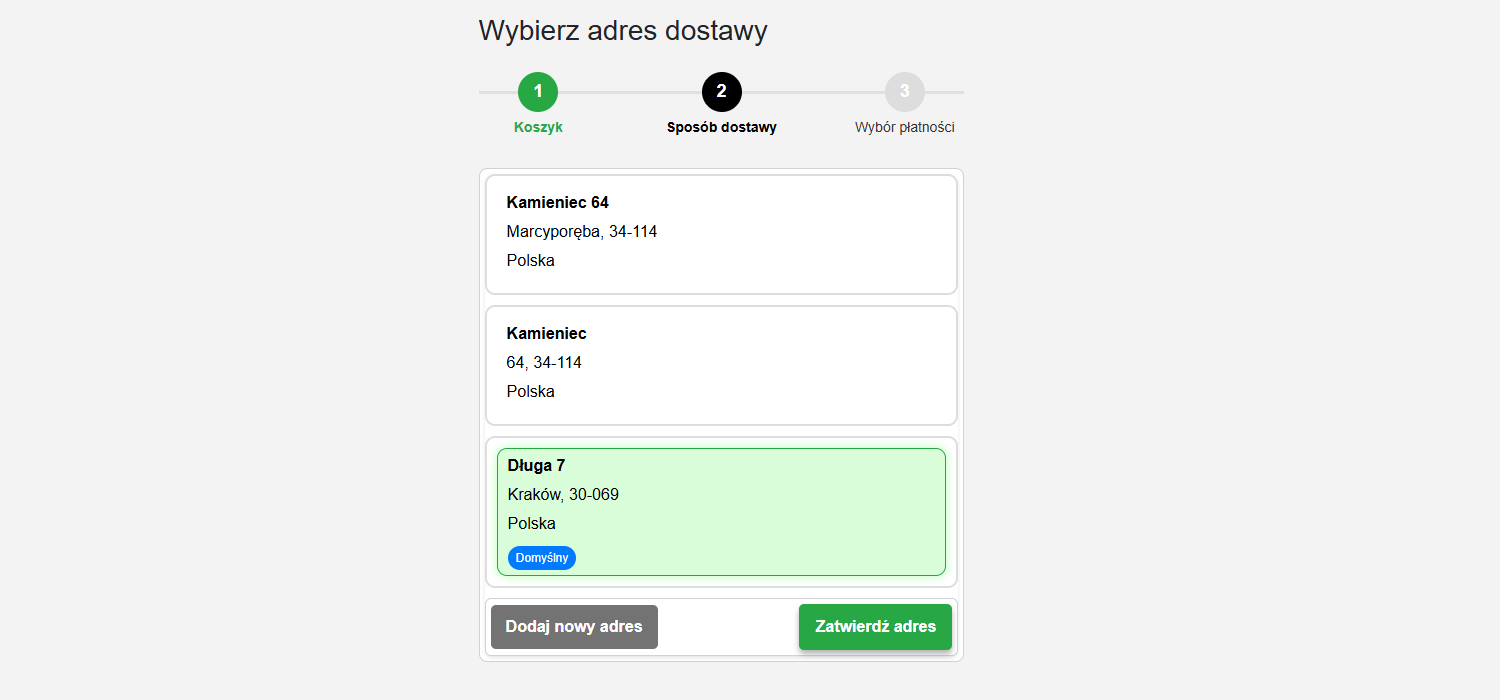
\includegraphics[width=1.0\columnwidth]{screens/address_selection.png}
    \caption{Widok wyboru adresu dostawy. \emph{Źródło: opracowanie własne.}}
    \label{fig:address_selection}
\end{figure}
\paragraph{Dodawanie nowego adresu}
Użytkownik ma możliwość dodania nowego adresu poprzez kliknięcie przycisku „Dodaj nowy adres”. Po kliknięciu otwiera się formularz zawierający pola:
\begin{itemize}
    \item \textbf{Ulica} – wprowadź nazwę ulicy i numer domu/mieszkania,
    \item \textbf{Miasto} – podaj nazwę miejscowości,
    \item \textbf{Kod pocztowy} – wpisz kod pocztowy w odpowiednim formacie,
    \item \textbf{Kraj} – wybierz kraj z listy rozwijanej.
\end{itemize}
Po wypełnieniu formularza użytkownik dodaje adres, klikając przycisk „Dodaj adres” znajdujący się na dole formularza.
\begin{figure}[H]
    \centering
    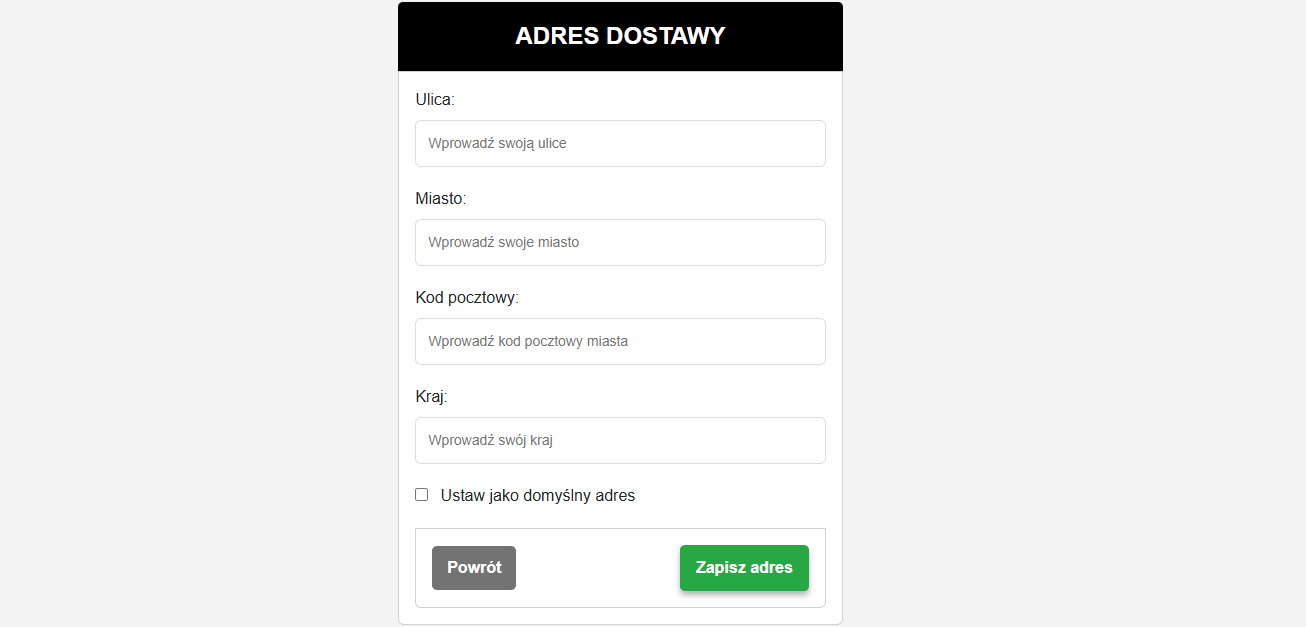
\includegraphics[width=1.0\columnwidth]{screens/add_address_form.png}
    \caption{Formularz dodawania nowego adresu. \emph{Źródło: opracowanie własne.}}
    \label{fig:add_address_form}
\end{figure}
\paragraph{Dodawanie adresu z menu profilu}
Adres można również dodać z poziomu menu rozwijanego „Profil” w górnym pasku nawigacyjnym. Po kliknięciu opcji „Dodaj adres” użytkownik zostaje przeniesiony do strony formularza, gdzie może wprowadzić dane adresowe. Na tej stronie można również zaznaczyć, czy adres ma być ustawiony jako domyślny dla przyszłych zakupów.
\begin{figure}[H]
    \centering
    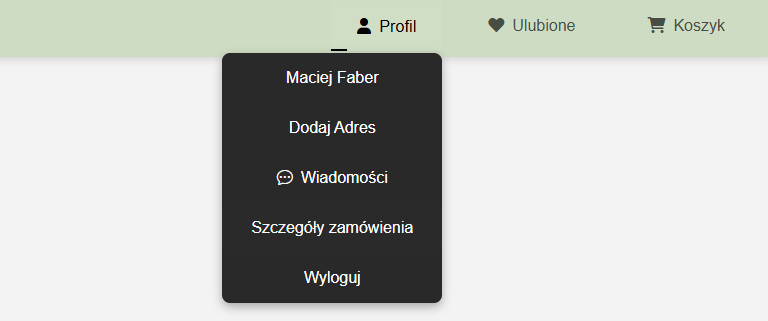
\includegraphics[width=1.0\columnwidth]{screens/profile_add_address.png}
    \caption{Dodanie adresu z poziomu zakładki "Profil". \emph{Źródło: opracowanie własne.}}
    \label{fig:profile_add_address}
\end{figure}





\subsubsection{Wybór płatności}
Po wyborze adresu dostawy użytkownik przechodzi do widoku wyboru metody płatności. System obsługuje trzy metody płatności, które można wybrać za pomocą formularza.

\paragraph{Dostępne metody płatności}
Użytkownik ma do wyboru następujące metody płatności:
\begin{itemize}
    \item \textbf{Karta kredytowa/debetowa} – użytkownik wprowadza dane karty, takie jak:
    \begin{itemize}
        \item Numer karty,
        \item Imię i nazwisko posiadacza karty,
        \item Datę ważności karty,
        \item Kod CVV.
    \end{itemize}
    \item \textbf{Blik} – użytkownik wpisuje sześciocyfrowy kod wygenerowany w aplikacji bankowej i zatwierdza płatność.

    \item \textbf{Płatność za pobraniem} – użytkownik wybiera tę opcję, jeśli chce zapłacić przy odbiorze przesyłki.
\end{itemize}

\begin{figure}[H]
    \centering
    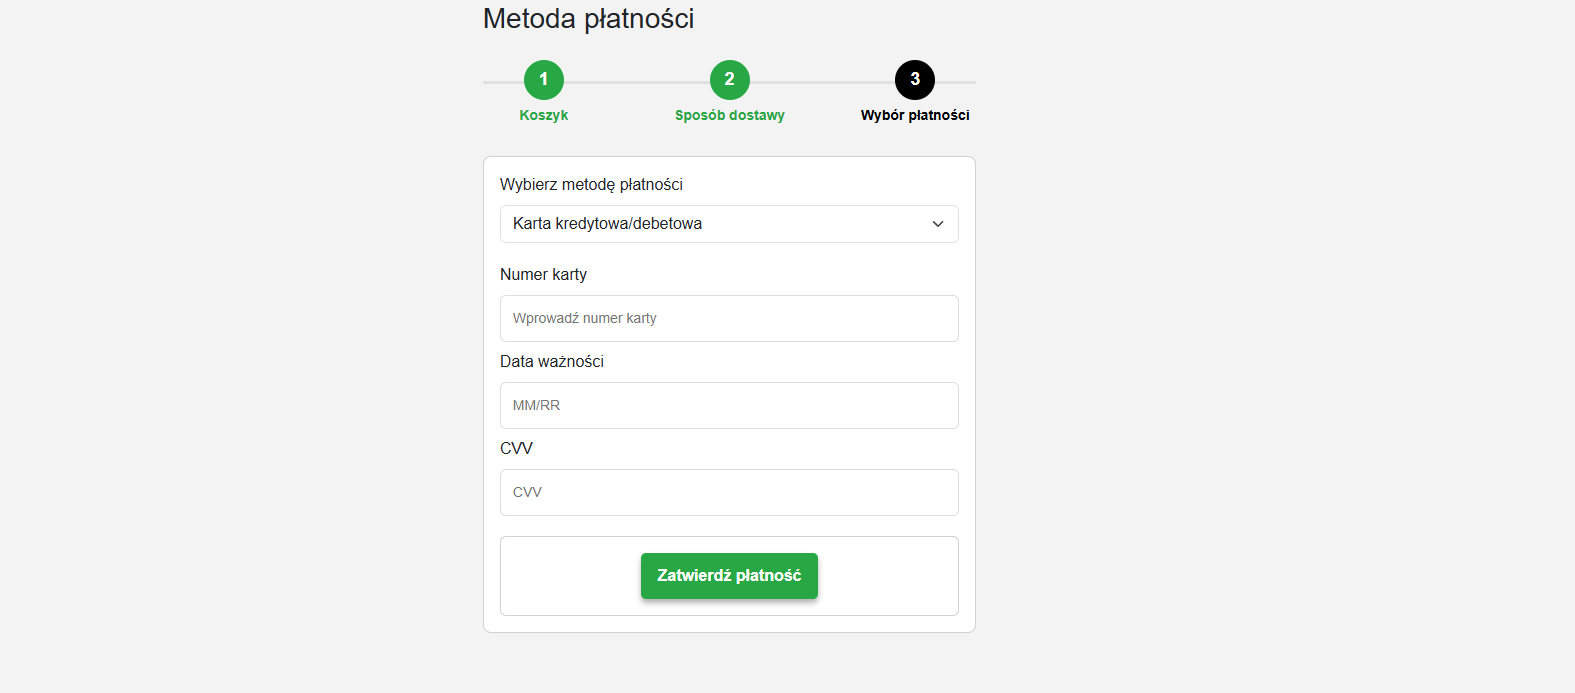
\includegraphics[width=1.0\columnwidth]{screens/payment_method.png}
    \caption{Widok wyboru metody płatności. \emph{Źródło: opracowanie własne.}}
    \label{fig:payment_method}
\end{figure}

\paragraph{Zatwierdzenie płatności}
Po wybraniu jednej z metod płatności użytkownik klika przycisk „Zatwierdź płatność”. Po pomyślnym zatwierdzeniu użytkownik zostaje przeniesiony do widoku szczegółów zamówienia, gdzie znajdują się informacje podsumowujące złożone zamówienie.





\subsubsection{Widok szczegółów zamówienia}
Po zakończeniu wyboru płatności użytkownik zostaje przekierowany do widoku szczegółów zamówienia. Zamówienie przechodzi przez następujące statusy:
\begin{itemize}
    \item \textbf{Utworzono} – Utworzone,
    \item \textbf{Przetwarzanie} – Przetwarzanie,
    \item \textbf{W dostawie} – W dostawie,
    \item \textbf{Gotowe do odbioru} – Gotowe do odbioru,
    \item \textbf{Zakończone} – Zakończone.
\end{itemize}

\paragraph{Elementy widoku szczegółów zamówienia}
Widok szczegółów zamówienia zawiera następujące informacje:
\begin{itemize}
    \item \textbf{ID zamówienia} – unikalny identyfikator zamówienia,
    \item \textbf{Status},
    \item \textbf{Łączna kwota zamówienia},
    \item \textbf{Data utworzenia zamówienia},
    \item \textbf{Adres dostawy},
    \item \textbf{Metoda płatności}.
\end{itemize}

Poniżej głównych informacji znajduje się lista produktów zamówionych przez użytkownika. Przy każdym produkcie widoczne są następujące dane:
\begin{itemize}
    \item Nazwa produktu,
    \item Cena produktu,
    \item Informacja, że ocena produktu będzie dostępna po zakończeniu dostawy.
\end{itemize}
\begin{figure}[H]
    \centering
    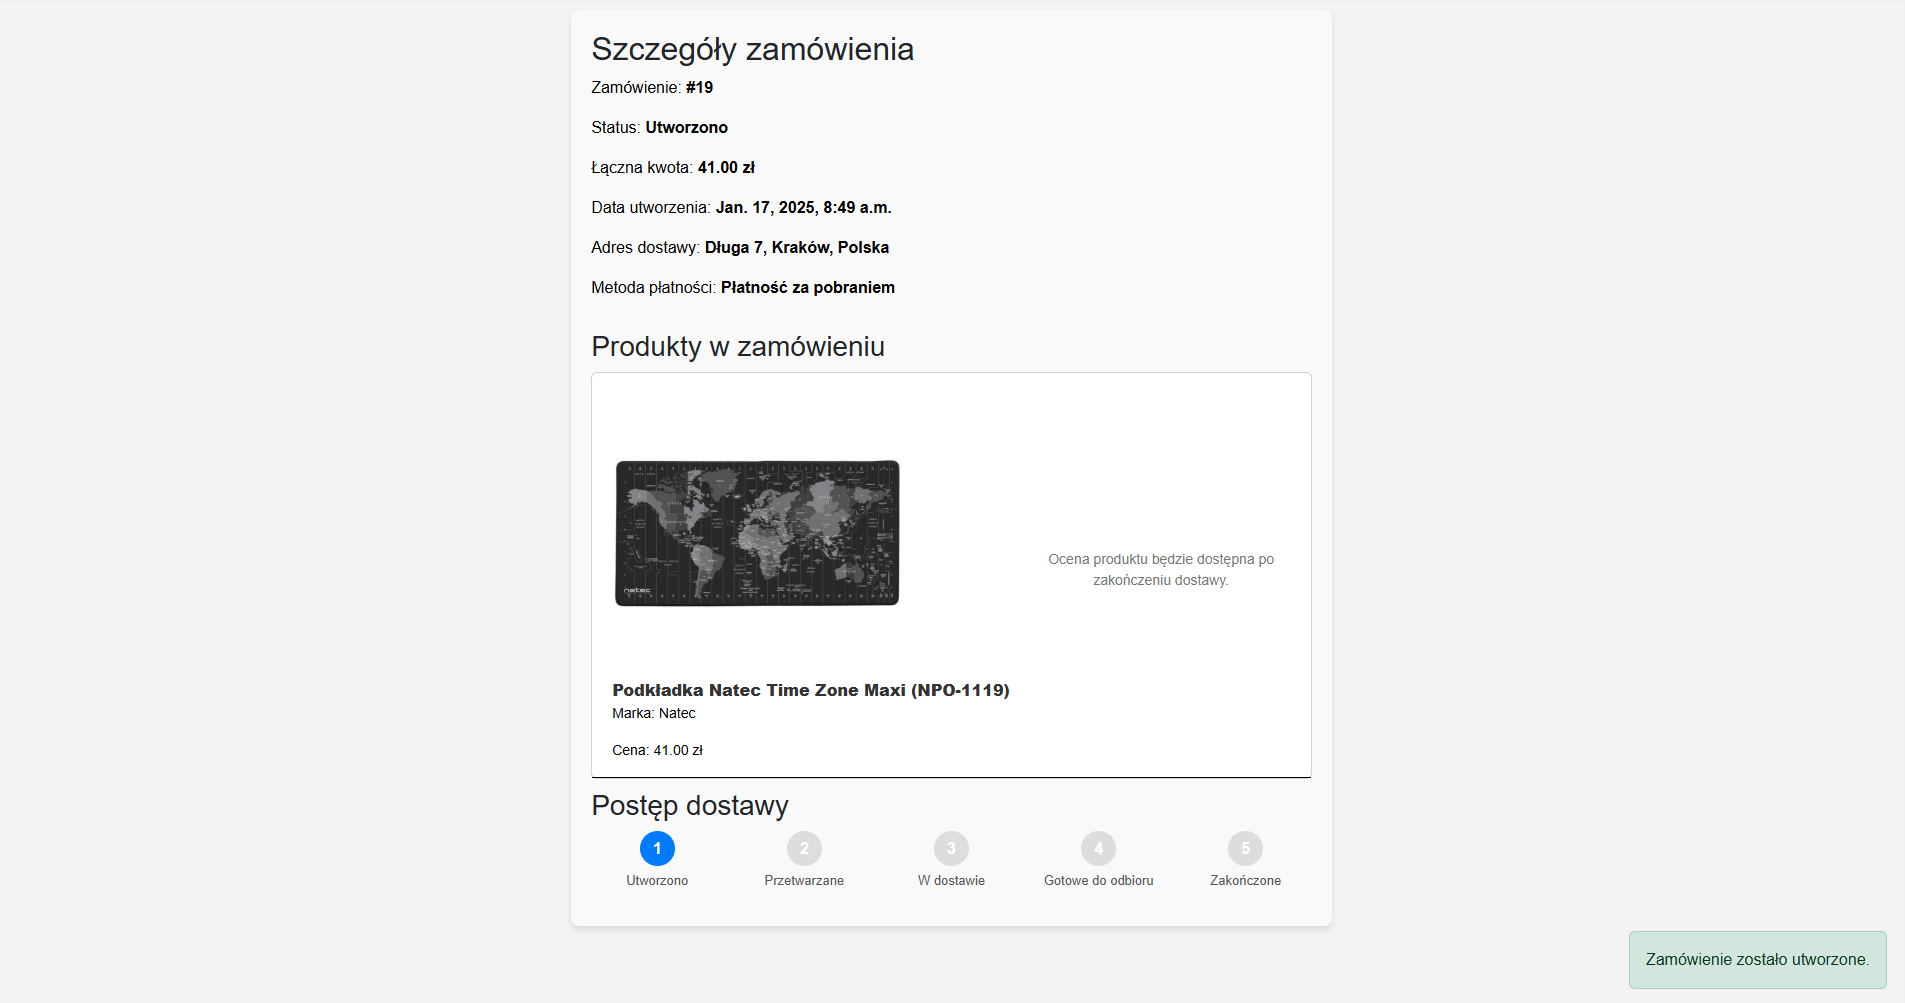
\includegraphics[width=1.0\columnwidth]{screens/order_status_create.png}
    \caption{Widok szczegółów zamówienia ze statusem "Utworzono". \emph{Źródło: opracowanie własne.}}
    \label{fig:order_status_create}
\end{figure}
\paragraph{Pasek postępu dostawy}
Na dole widoku znajduje się pasek postępu, który ilustruje aktualny status zamówienia. Pasek wskazuje jeden z pięciu statusów zamówienia, zaczynając od „Utworzono”, aż po „Zakończone”.

\paragraph{Ocena produktów po zakończeniu dostawy}
Gdy zamówienie osiągnie status „Zakończone”, przy każdym produkcie pojawia się formularz umożliwiający ocenę produktu. Formularz zawiera:
\begin{itemize}
    \item Pole wyboru oceny w skali 1-5 (gwiazdki),
    \item Pole tekstowe na komentarz do produktu,
    \item Przycisk „Wyślij ocenę” – wysyłający ocenę i zapisujący ją w systemie.
\end{itemize}

\paragraph{Dodawanie produktów do polubionych}
Pod listą produktów znajduje się również przycisk umożliwiający dodanie produktów do listy polubionych. Po kliknięciu produkt zostaje zapisany na liście ulubionych użytkownika.

\begin{figure}[H]
    \centering
    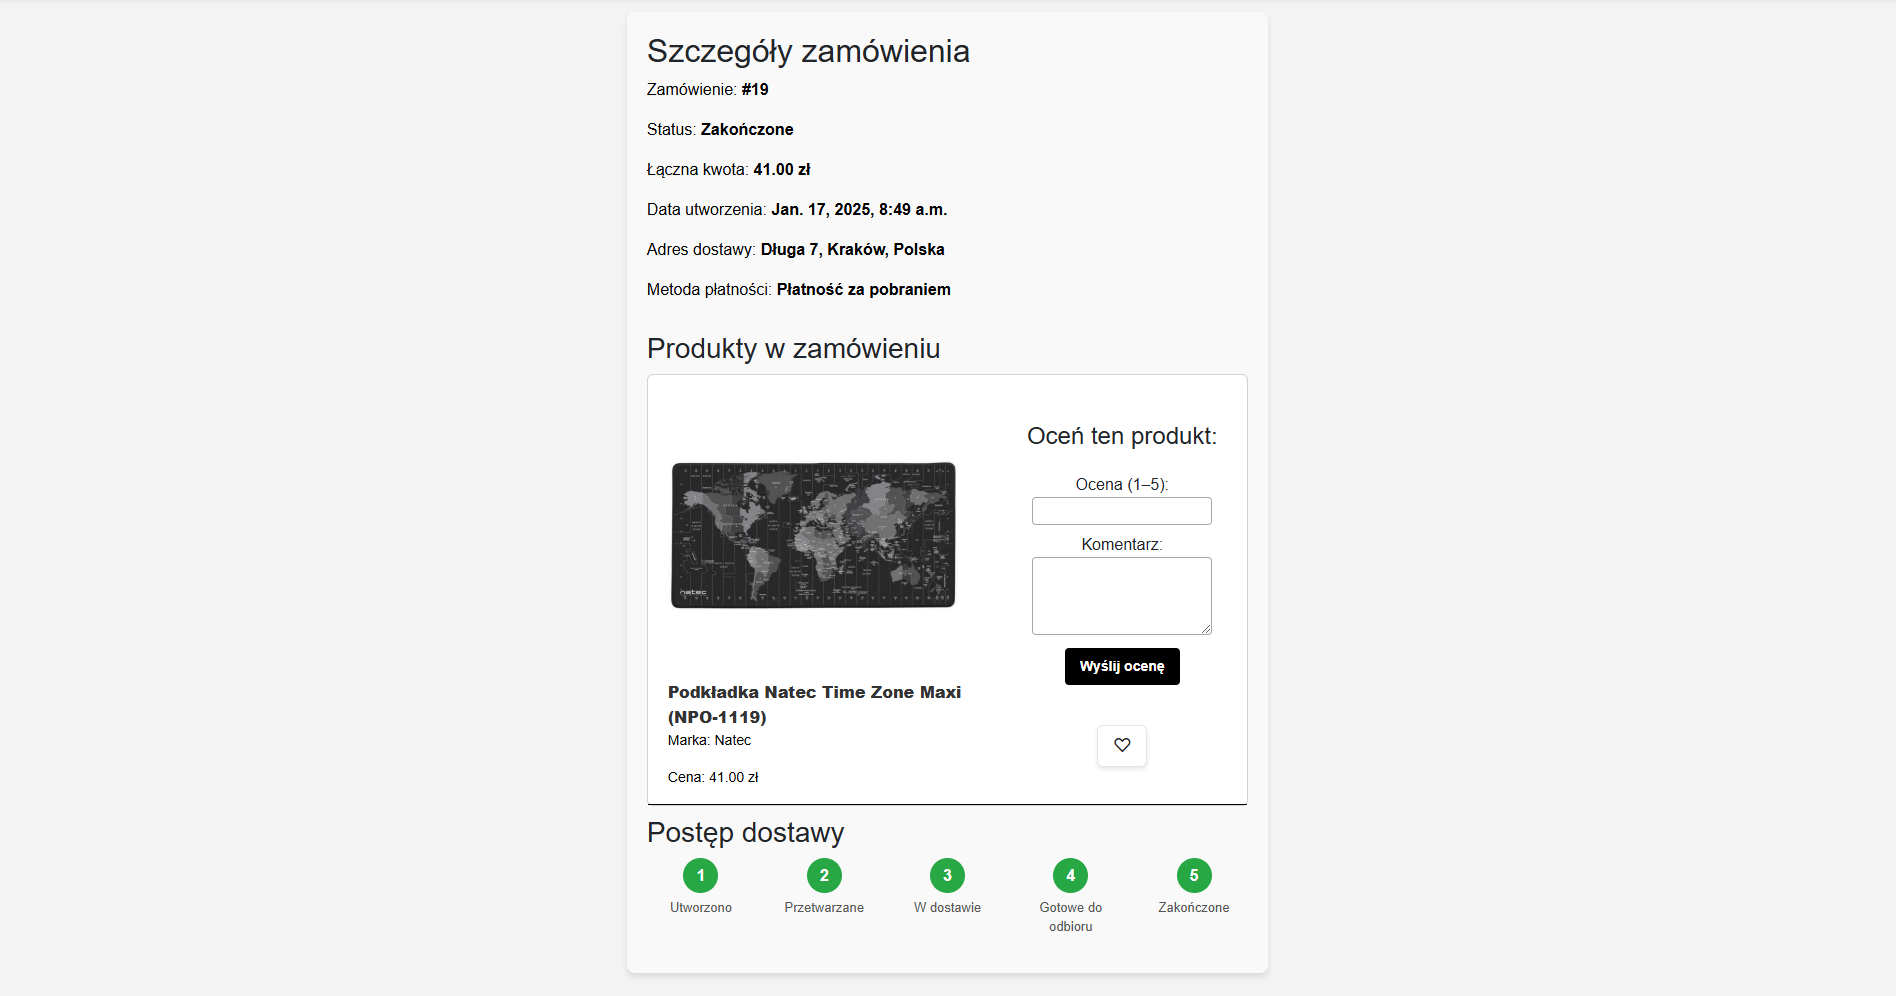
\includegraphics[width=1.0\columnwidth]{screens/order_status_finish.png}
    \caption{Widok szczegółów zamówienia ze statusem "Zakończone". \emph{Źródło: opracowanie własne.}}
    \label{fig:order_status_finish}
\end{figure}




\subsubsection{Widok wiadomości}
Widok wiadomości umożliwia użytkownikowi przeglądanie i zarządzanie konwersacjami związanymi z jego zamówieniami. Każde zamówienie generuje dwie osobne konwersacje:
\begin{itemize}
    \item \textbf{Status zamówienia} – automatyczne aktualizacje informujące o postępie realizacji zamówienia,
    \item \textbf{Konwersacja z administratorem} – umożliwia bezpośredni kontakt z administratorem w sprawach dotyczących zamówienia.
\end{itemize}

\paragraph{Elementy widoku wiadomości}
Widok wiadomości składa się z dwóch głównych sekcji:
\begin{itemize}
    \item \textbf{Lista konwersacji} – widoczna po lewej stronie ekranu. Wyświetlane są tutaj wszystkie konwersacje przypisane do zamówień użytkownika. Każda konwersacja jest opisana za pomocą:
    \begin{itemize}
        \item ID zamówienia,
        \item Typu konwersacji (np. „Status zamówienia” lub „Rozmowa z administratorem”),
    \end{itemize}
    \item \textbf{Treść wybranej konwersacji} – widoczna po prawej stronie ekranu. Wyświetlane są wiadomości wymienione w ramach wybranej konwersacji. Każda wiadomość zawiera:
    \begin{itemize}
        \item Nadawcę wiadomości (użytkownik lub administrator),
        \item Treść wiadomości,
        \item Godzinę wysłania wiadomości.
    \end{itemize}
\end{itemize}

\paragraph{Wysyłanie wiadomości do administratora}
Użytkownik może wysłać wiadomość do administratora w konwersacji przypisanej do danego zamówienia. W dolnej części widoku wiadomości znajduje się pole tekstowe, w którym użytkownik może wpisać treść wiadomości, oraz przycisk „Wyślij”. Po kliknięciu wiadomość jest wysyłana do administratora i zapisywana w systemie.

\paragraph{Przykład działania}
1. Użytkownik wybiera zamówienie z listy konwersacji po lewej stronie.
2. Po kliknięciu wybranego zamówienia, po prawej stronie ekranu wyświetlane są wszystkie wiadomości związane z daną konwersacją.
3. Użytkownik może wpisać wiadomość w polu tekstowym i kliknąć „Wyślij”, aby dodać nową wiadomość do konwersacji.

\begin{figure}[H]
    \centering
    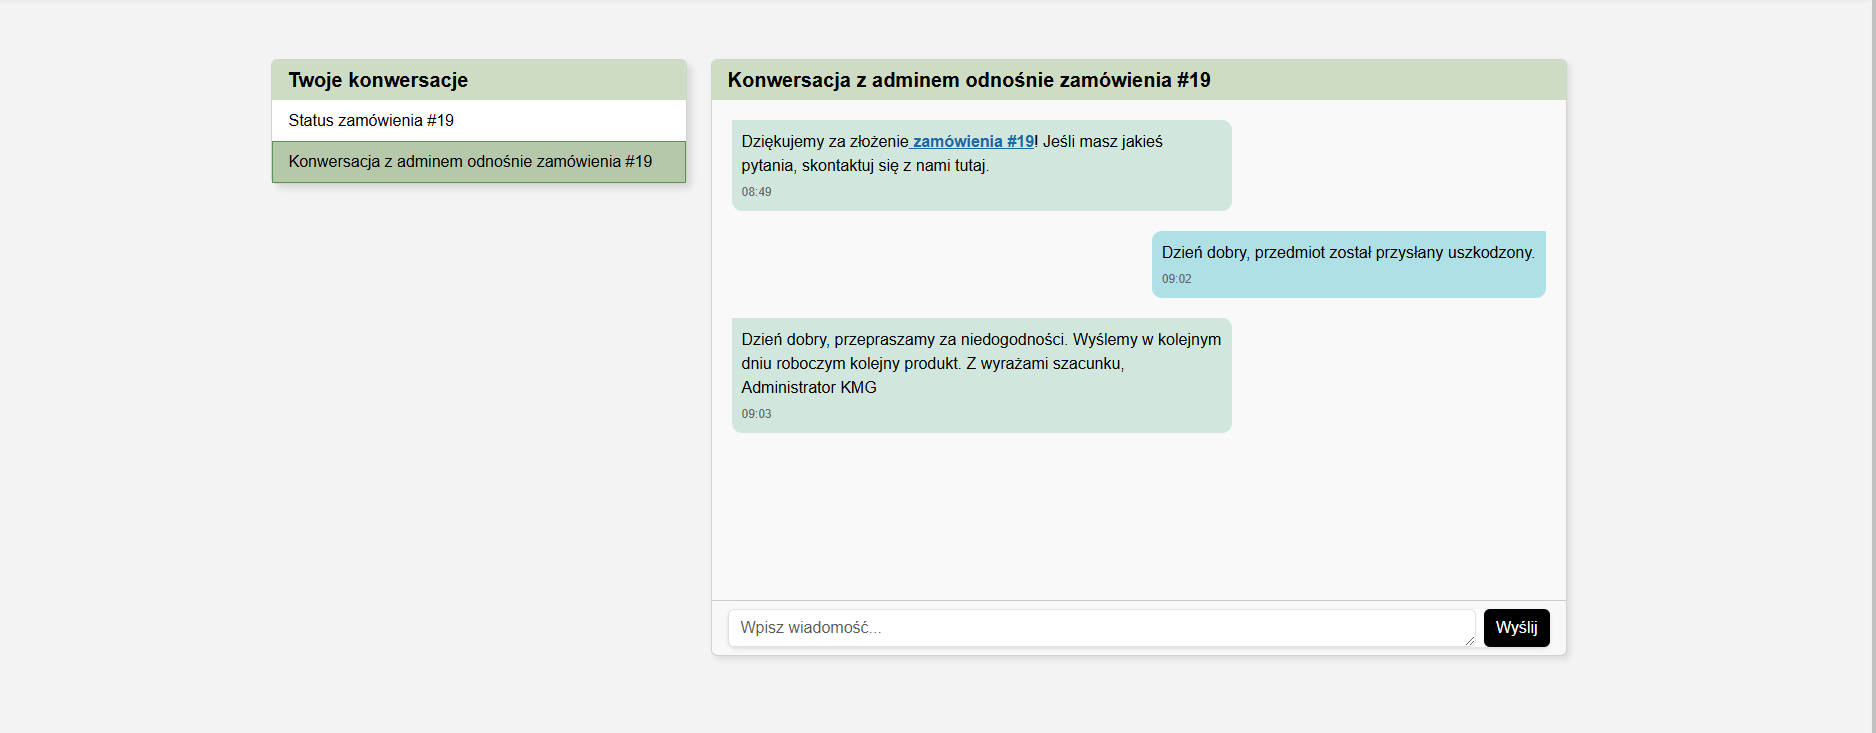
\includegraphics[width=1.0\columnwidth]{screens/messages_view.png}
    \caption{Widok wiadomości w zakładce Profil. \emph{Źródło: opracowanie własne.}}
    \label{fig:messages_view}
\end{figure}



\subsubsection{Widok zamówień}
Widok zamówień w zakładce „Profil” pozwala użytkownikowi na przeglądanie wszystkich swoich zamówień. Każde zamówienie zawiera podstawowe informacje oraz przycisk umożliwiający przejście do szczegółów zamówienia.

\paragraph{Elementy widoku zamówień}
Widok zamówień przedstawia listę wszystkich zamówień użytkownika w formie tabeli lub listy. Dla każdego zamówienia wyświetlane są następujące informacje:
\begin{itemize}
    \item \textbf{ID zamówienia} – unikalny identyfikator zamówienia,
    \item \textbf{Data zamówienia} – data, kiedy zamówienie zostało utworzone,
    \item \textbf{Status zamówienia} – aktualny status zamówienia, np. „Utworzono”, „Przetwarzanie”, „W dostawie”, „Gotowe do odbioru” lub „Zakończone”.
\end{itemize}

\paragraph{Przycisk „Szczegóły zamówienia”}
Obok każdego zamówienia znajduje się przycisk „Szczegóły zamówienia”. Kliknięcie przycisku powoduje przejście do widoku szczegółów zamówienia, gdzie użytkownik może zobaczyć pełne informacje o zamówieniu, w tym listę zamówionych produktów, adres dostawy oraz metodę płatności.

\paragraph{Przykład działania}
1. Użytkownik otwiera zakładkę „Profil” i wybiera sekcję „Zamówienia”.
2. Na ekranie wyświetlana jest lista wszystkich zamówień użytkownika, posortowana według daty (od najnowszego do najstarszego).
3. Użytkownik może kliknąć przycisk „Szczegóły zamówienia” przy wybranym zamówieniu, aby przejść do szczegółowego widoku zamówienia.

\begin{figure}[H]
    \centering
    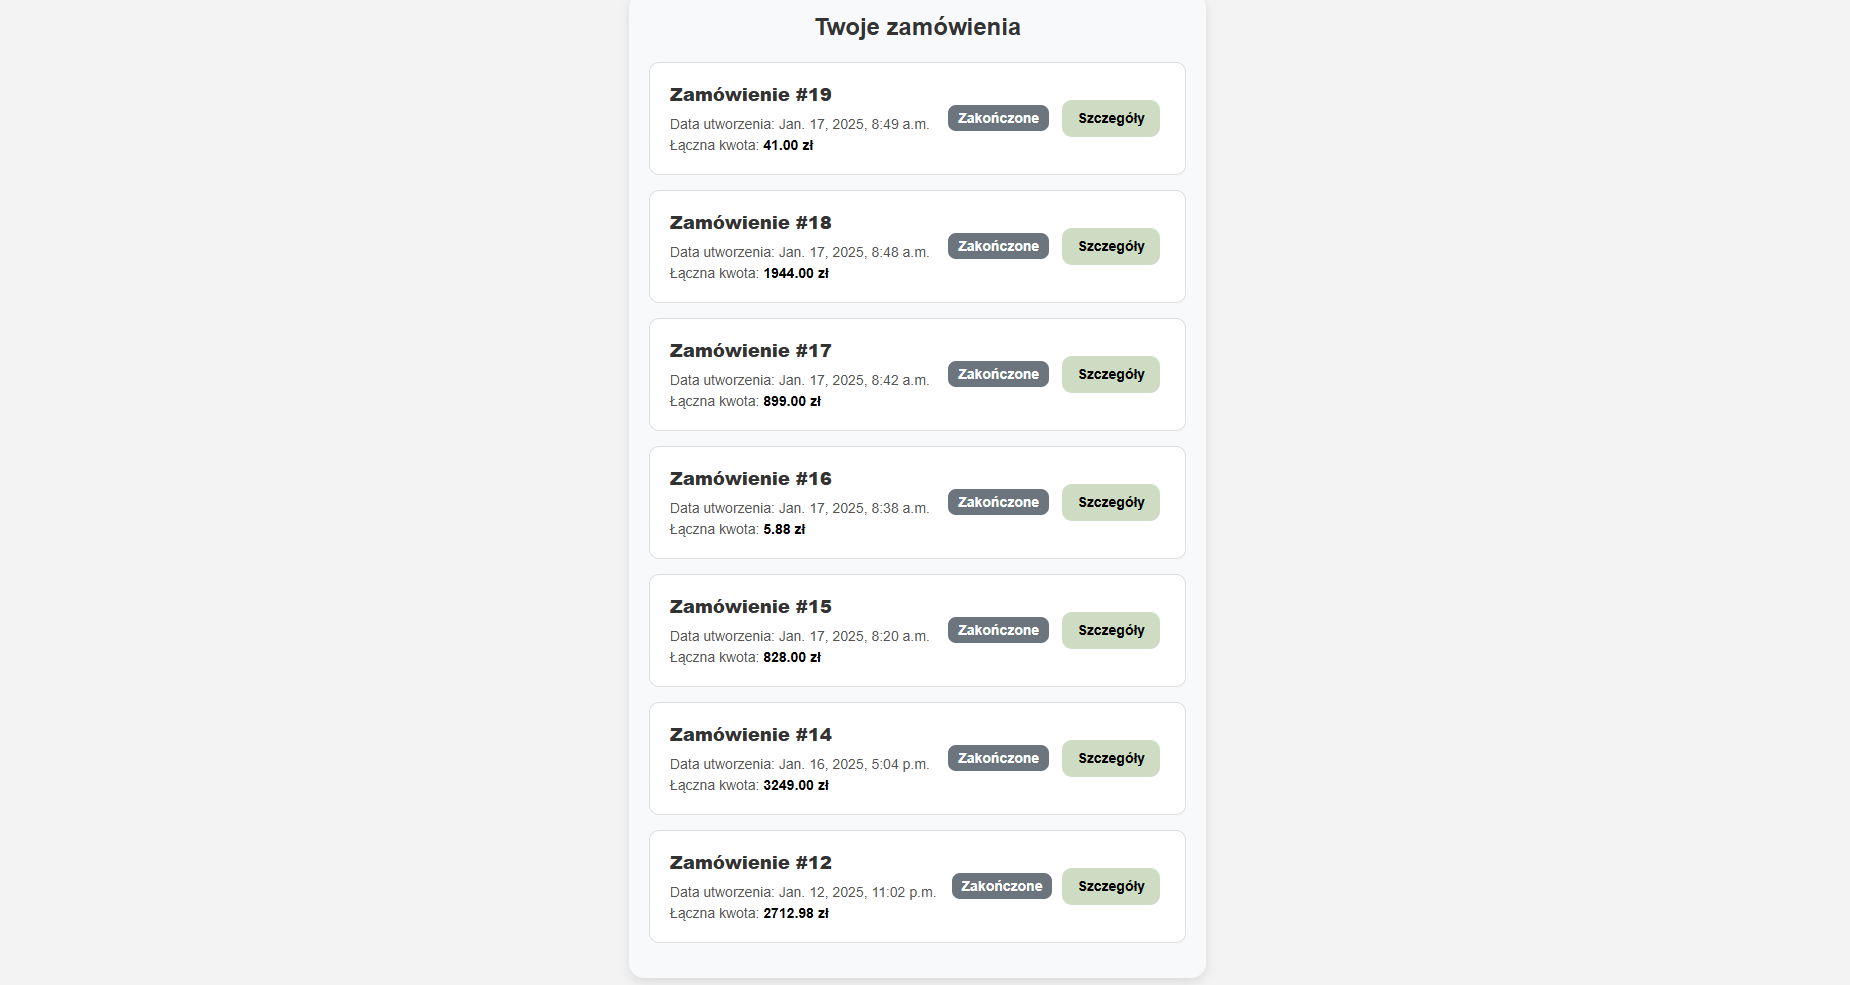
\includegraphics[width=1.0\columnwidth]{screens/orders_view.png}
    \caption{Widok zamówień w zakładce Profil. \emph{Źródło: opracowanie własne.}}
    \label{fig:orders_view}
\end{figure}




\subsubsection{Widok Profil}
Widok „Profil” pozwala użytkownikowi na przeglądanie i edytowanie swoich danych osobowych podanych podczas rejestracji. Wszystkie zmiany wprowadzone w danych użytkownika wymagają potwierdzenia hasłem.

\paragraph{Przycisk „Profil” w zakładce Profil}
W zakładce „Profil” znajduje się przycisk z imieniem i nazwiskiem użytkownika. Po jego kliknięciu użytkownik zostaje przeniesiony do szczegółowego widoku swojego profilu.

\paragraph{Dane użytkownika}
Na widoku profilu wyświetlane są wszystkie dane osobowe użytkownika wprowadzone podczas rejestracji, podzielone na trzy sekcje:
\begin{enumerate}
    \item \textbf{Dane podstawowe}:
    \begin{itemize}
        \item Imię,
        \item Nazwisko,
        \item Numer telefonu,
        \item Data urodzenia.
    \end{itemize}
    \item \textbf{Adres e-mail} – używany do logowania i komunikacji.
    \item \textbf{Zmiana hasła} – pozwala na aktualizację hasła użytkownika.
\end{enumerate}

\begin{figure}[H]
    \centering
    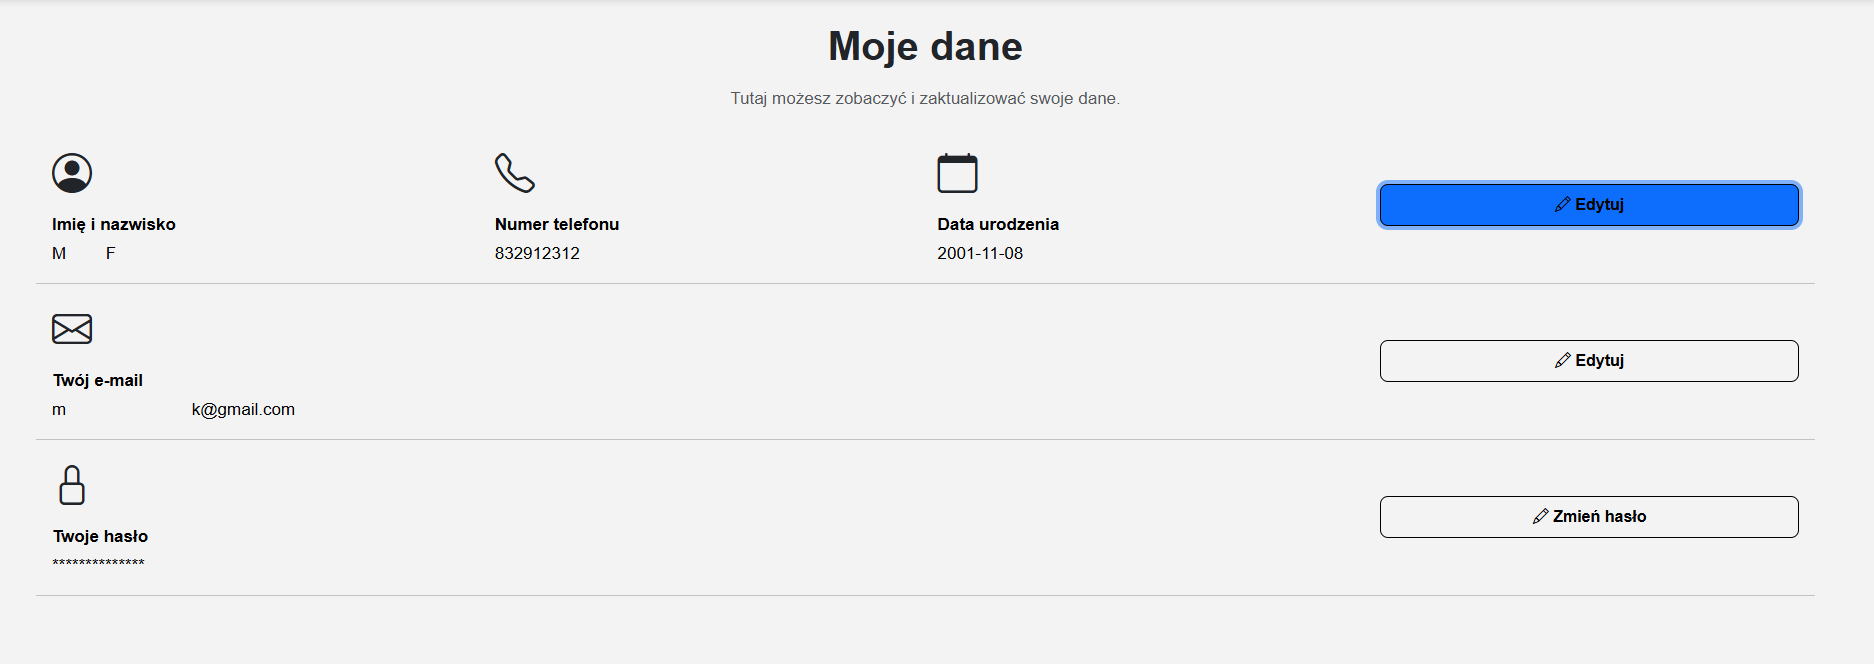
\includegraphics[width=1.0\columnwidth]{screens/profile_edit.png}
    \caption{Widok Profil z danymi użytkownika i sekcjami edytowania. \emph{Źródło: opracowanie własne.}}
    \label{fig:profile_edit}
\end{figure}

\paragraph{Edycja danych}
Każda sekcja danych posiada przycisk „Edytuj”. Po kliknięciu przycisku użytkownik może edytować dane w danej sekcji. Szczegóły edycji:
\begin{itemize}
    \item Po kliknięciu „Edytuj” wyświetlają się pola wejściowe do modyfikacji danych.
    \item Po wprowadzeniu zmian użytkownik musi wpisać swoje obecne hasło w celu ich zatwierdzenia.
    \item Po kliknięciu przycisku „Zapisz” system weryfikuje hasło i wprowadzone dane:
    \begin{itemize}
        \item Jeśli hasło lub dane są nieprawidłowe, wyświetlany jest odpowiedni komunikat o błędzie.
        \item Jeśli wszystko jest poprawne, zmiany są zapisywane, a użytkownik otrzymuje komunikat potwierdzający.
    \end{itemize}
\end{itemize}

\paragraph{Podział na sekcje edytowania danych}
\begin{itemize}
    \item \textbf{Dane podstawowe}: Użytkownik może zmieniać imię, nazwisko, numer telefonu oraz datę urodzenia.
    
\begin{figure}[H]
    \centering
    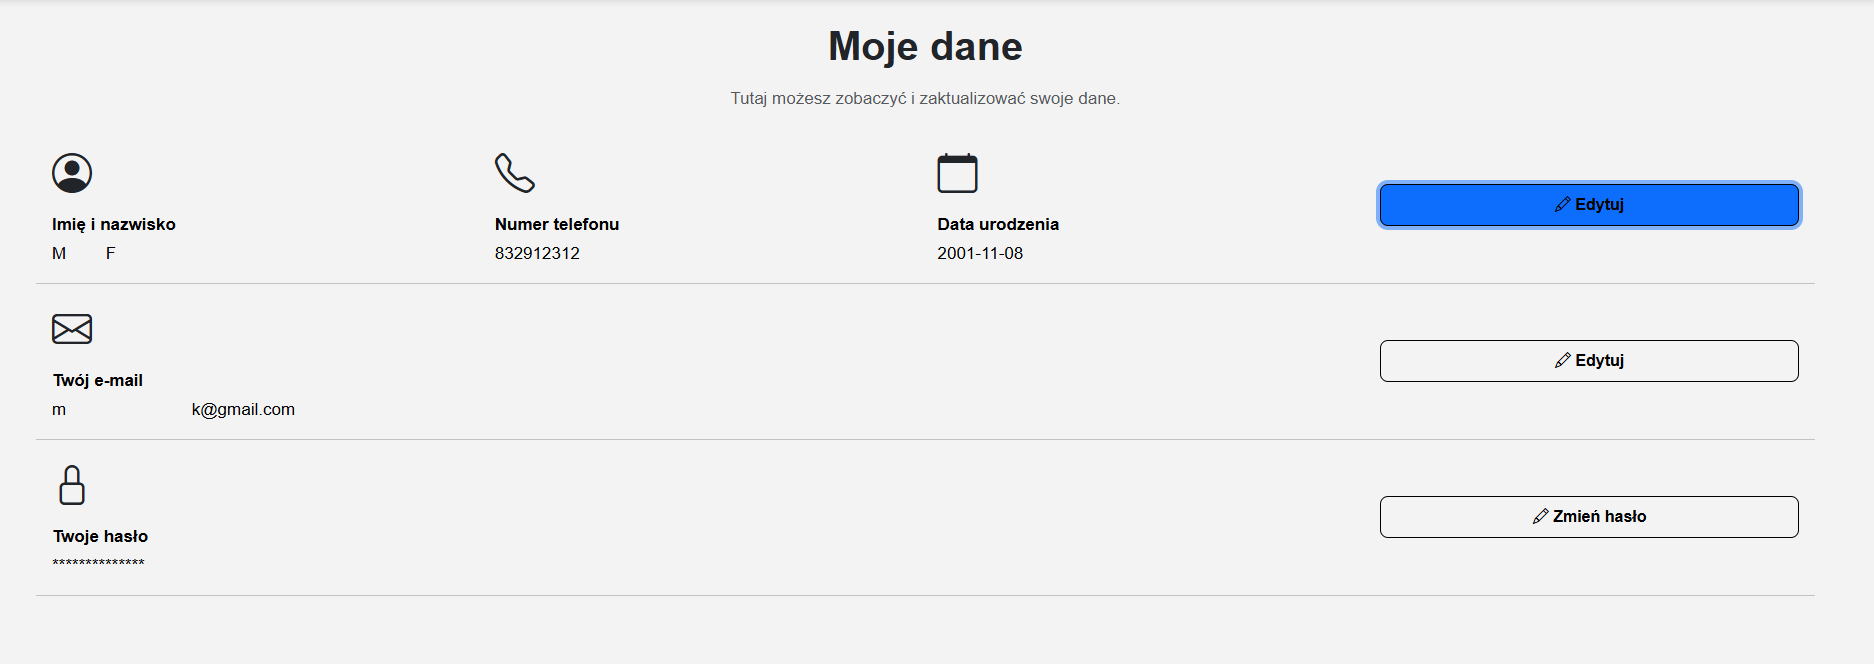
\includegraphics[width=1.0\columnwidth]{screens/profile_edit.png}
    \caption{Widok edycji danych podstawowych. \emph{Źródło: opracowanie własne.}}
    \label{fig:profile_edit_first}
\end{figure}

    \item \textbf{Adres e-mail}: Użytkownik może zaktualizować swój adres e-mail, który jest używany do logowania oraz powiadomień.
    
\begin{figure}[H]
    \centering
    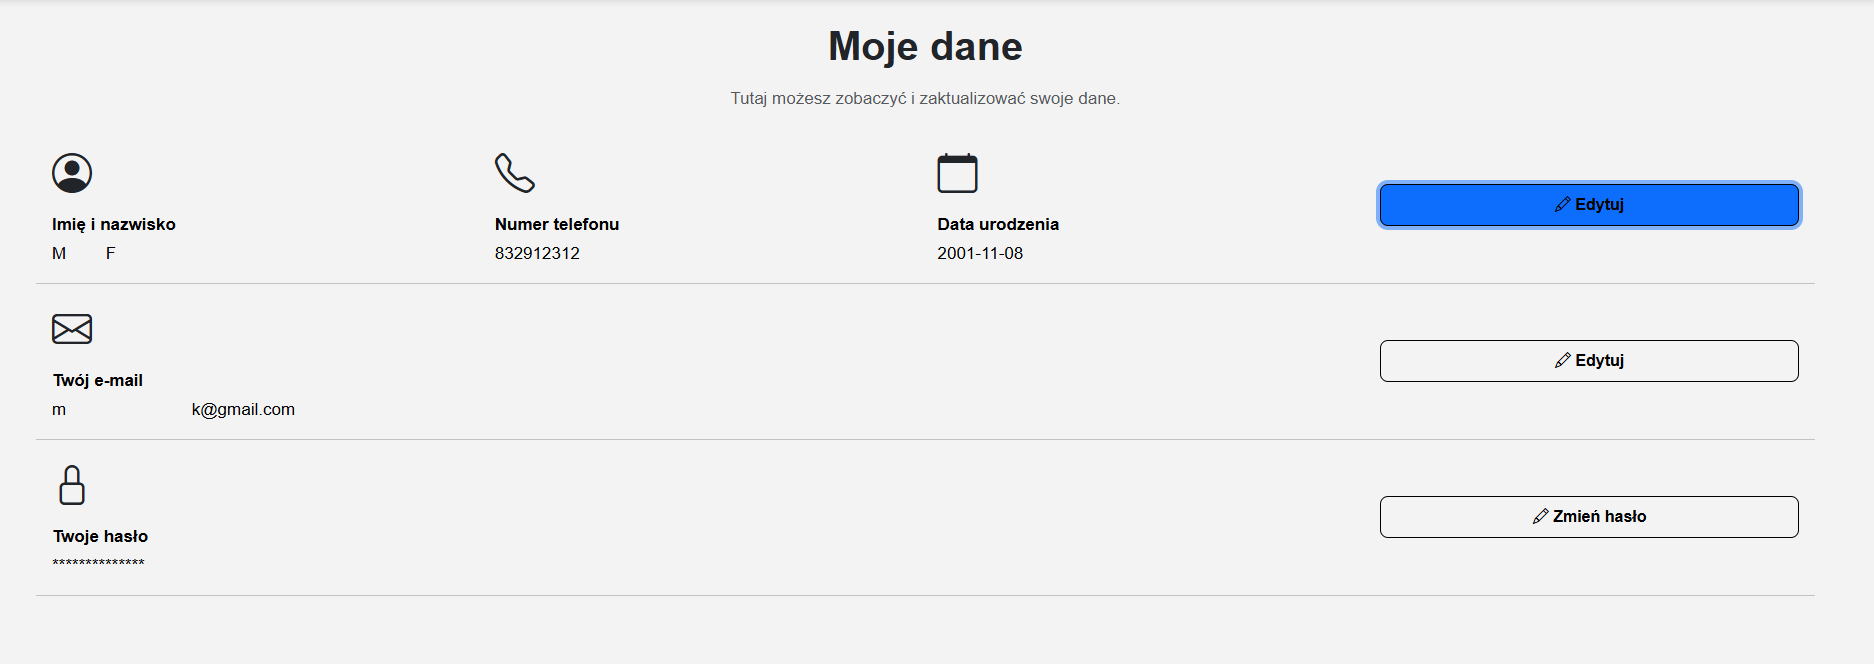
\includegraphics[width=1.0\columnwidth]{screens/profile_edit.png}
    \caption{Widok edycji adresu email. \emph{Źródło: opracowanie własne.}}
    \label{fig:profile_edit_email}
\end{figure}
    
    \item \textbf{Zmiana hasła}: Użytkownik wprowadza swoje aktualne hasło, nowe hasło oraz jego potwierdzenie. System sprawdza zgodność hasła z wymaganiami bezpieczeństwa.

    \begin{figure}[H]
        \centering
        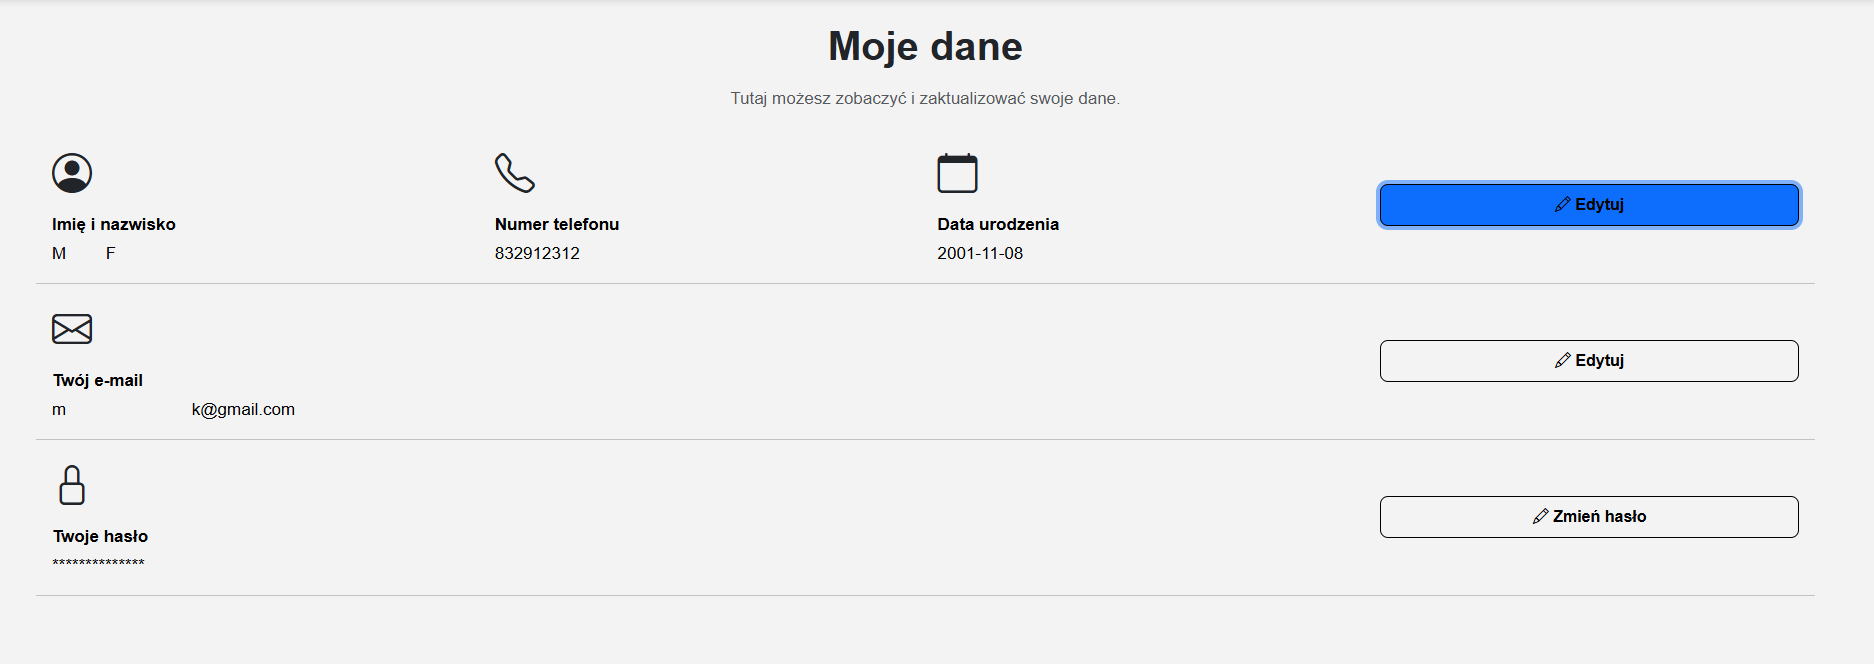
\includegraphics[width=1.0\columnwidth]{screens/profile_edit.png}
        \caption{Widok edycji hasła. \emph{Źródło: opracowanie własne.}}
        \label{fig:profile_password}
    \end{figure}
    
\end{itemize}





\subsubsection{Widok edycji opinii o produkcie}
Widok edycji opinii umożliwia użytkownikowi zmianę oceny i komentarza dodanych wcześniej do produktu. Edycja opinii jest dostępna poprzez szczegóły produktu.

\paragraph{Dostęp do edycji opinii}
Aby edytować swoją opinię, użytkownik:
\begin{enumerate}
    \item Przechodzi do szczegółowego widoku produktu.
    \item Klika w sekcję ocen produktu, gdzie wyświetlane są wszystkie opinie.
    \item Na pierwszym miejscu wyświetlana jest opinia użytkownika, jeśli została już wcześniej dodana. Obok opinii znajduje się przycisk „Edytuj opinię”.
\end{enumerate}
\begin{figure}[H]
    \centering
    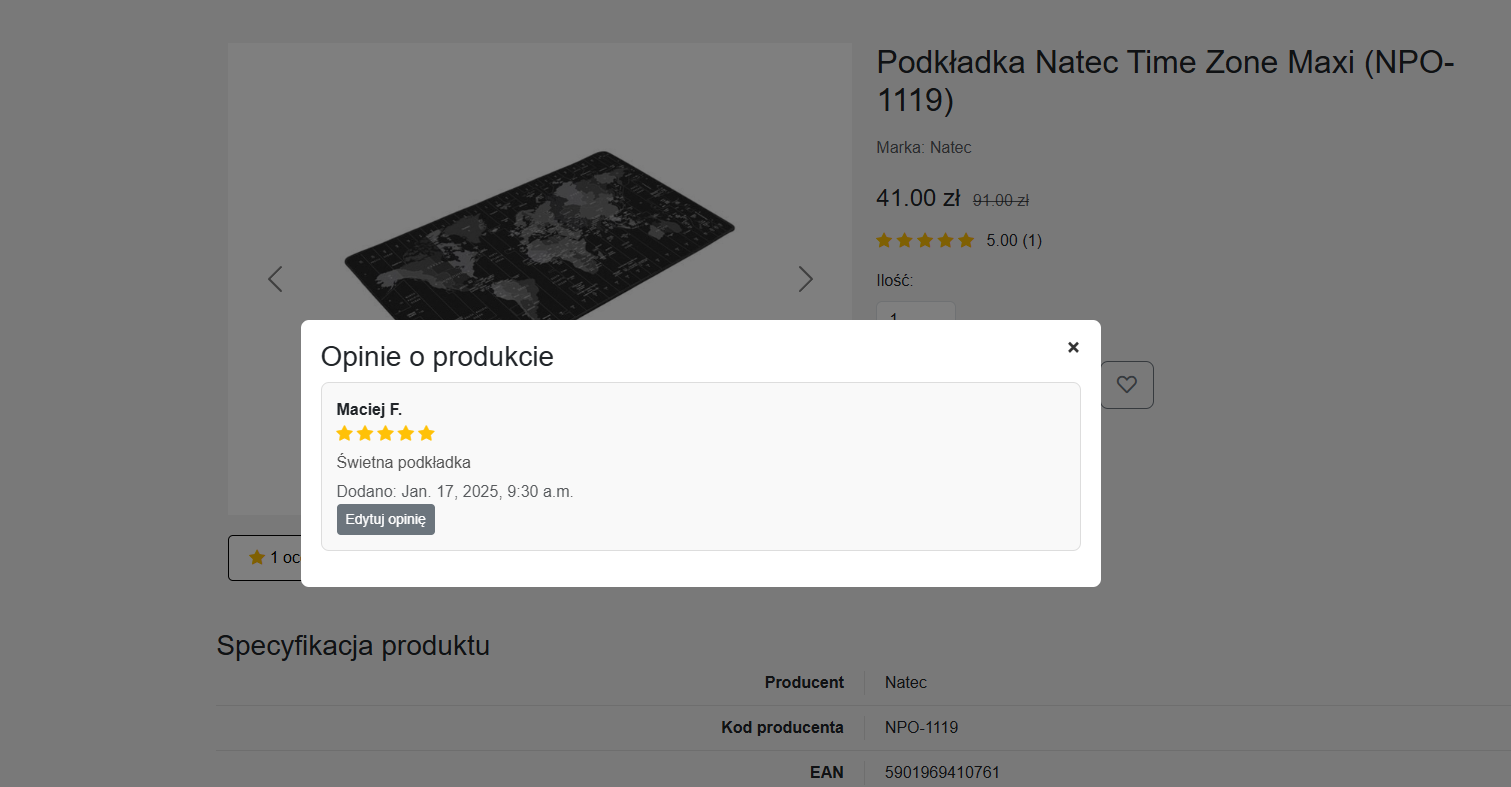
\includegraphics[width=1.0\columnwidth]{screens/opinion_user.png}
    \caption{Widok edycji opinii o produkcie. \emph{Źródło: opracowanie własne.}}
    \label{fig:opinion_user}
\end{figure}
\paragraph{Proces edycji opinii}
Po kliknięciu przycisku „Edytuj opinię” użytkownikowi wyświetlane są pola umożliwiające wprowadzenie zmian:
\begin{itemize}
    \item Pole do wyboru oceny w skali 1-5 (gwiazdki).
    \item Pole tekstowe na komentarz.
\end{itemize}
Pod polami edycji znajdują się dwa przyciski:
\begin{itemize}
    \item \textbf{Anuluj} – zamyka widok edycji bez zapisania zmian,
    \item \textbf{Zapisz zmiany} – zatwierdza zmiany i aktualizuje opinię w systemie.
\end{itemize}

\begin{figure}[H]
    \centering
    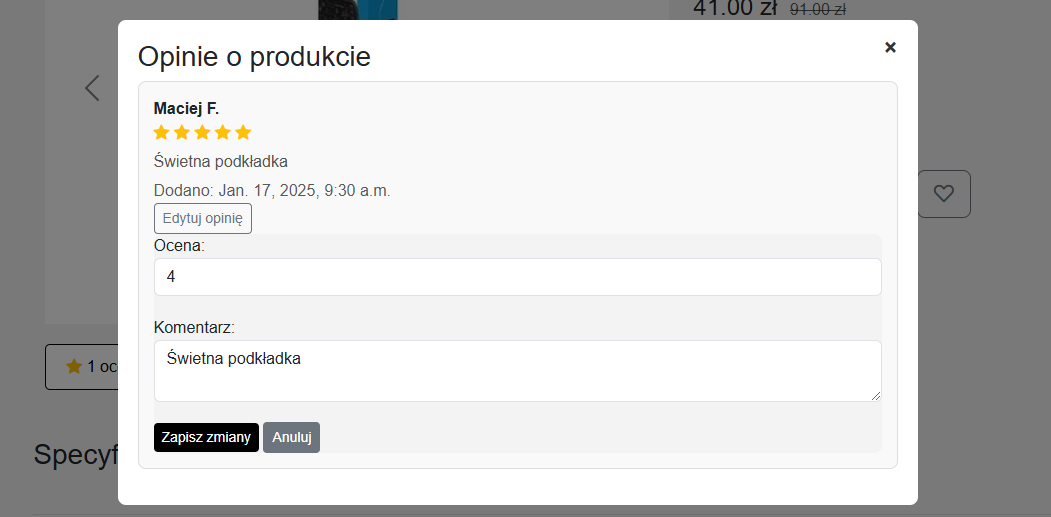
\includegraphics[width=1.0\columnwidth]{screens/opinion_user_edit.png}
    \caption{Widok edycji opinii o produkcie. \emph{Źródło: opracowanie własne.}}
    \label{fig:opinion_user_edit}
\end{figure}




\subsubsection{Filtrowanie i sortowanie produktów}
Widok listy produktów umożliwia użytkownikom zawężenie wyników za pomocą filtrów cenowych oraz uporządkowanie produktów według różnych kryteriów sortowania. Funkcje te pozwalają na łatwiejsze znalezienie odpowiednich produktów.

\paragraph{Filtrowanie po cenie}
Filtrowanie znajduje się pod listą kategorii w widoku produktów. Użytkownik może określić przedział cenowy, w jakim chcą przeglądać produkty:
\begin{itemize}
    \item Pole \textbf{od} – pozwala ustawić najniższą cenę produktów do wyświetlenia.
    \item Pole \textbf{do} – pozwala ustawić najwyższą cenę produktów do wyświetlenia.
\end{itemize}
Po wprowadzeniu wartości w pola filtrowania użytkownik klika przycisk „Zastosuj”, aby odświeżyć listę produktów zgodnie z ustawionym przedziałem cenowym. Jeśli żaden produkt nie spełnia kryteriów filtrowania, wyświetlany jest komunikat „Brak produktów w wybranym przedziale cenowym”.

\paragraph{Sortowanie produktów}
Funkcja sortowania znajduje się w prawym górnym rogu widoku listy produktów. Użytkownik może wybrać jedno z dostępnych kryteriów sortowania:
\begin{itemize}
    \item \textbf{Popularność} – produkty są sortowane według liczby polubień użytkowników, od najbardziej do najmniej popularnych.
    \item \textbf{Ocena} – produkty są sortowane według średniej oceny użytkowników, od najwyższej do najniższej.
    \item \textbf{Cena} – produkty są sortowane rosnąco (od najtańszych) lub malejąco (od najdroższych). Użytkownik może przełączać kolejność za pomocą strzałki obok opcji sortowania.
\end{itemize}

\begin{figure}[H]
    \centering
    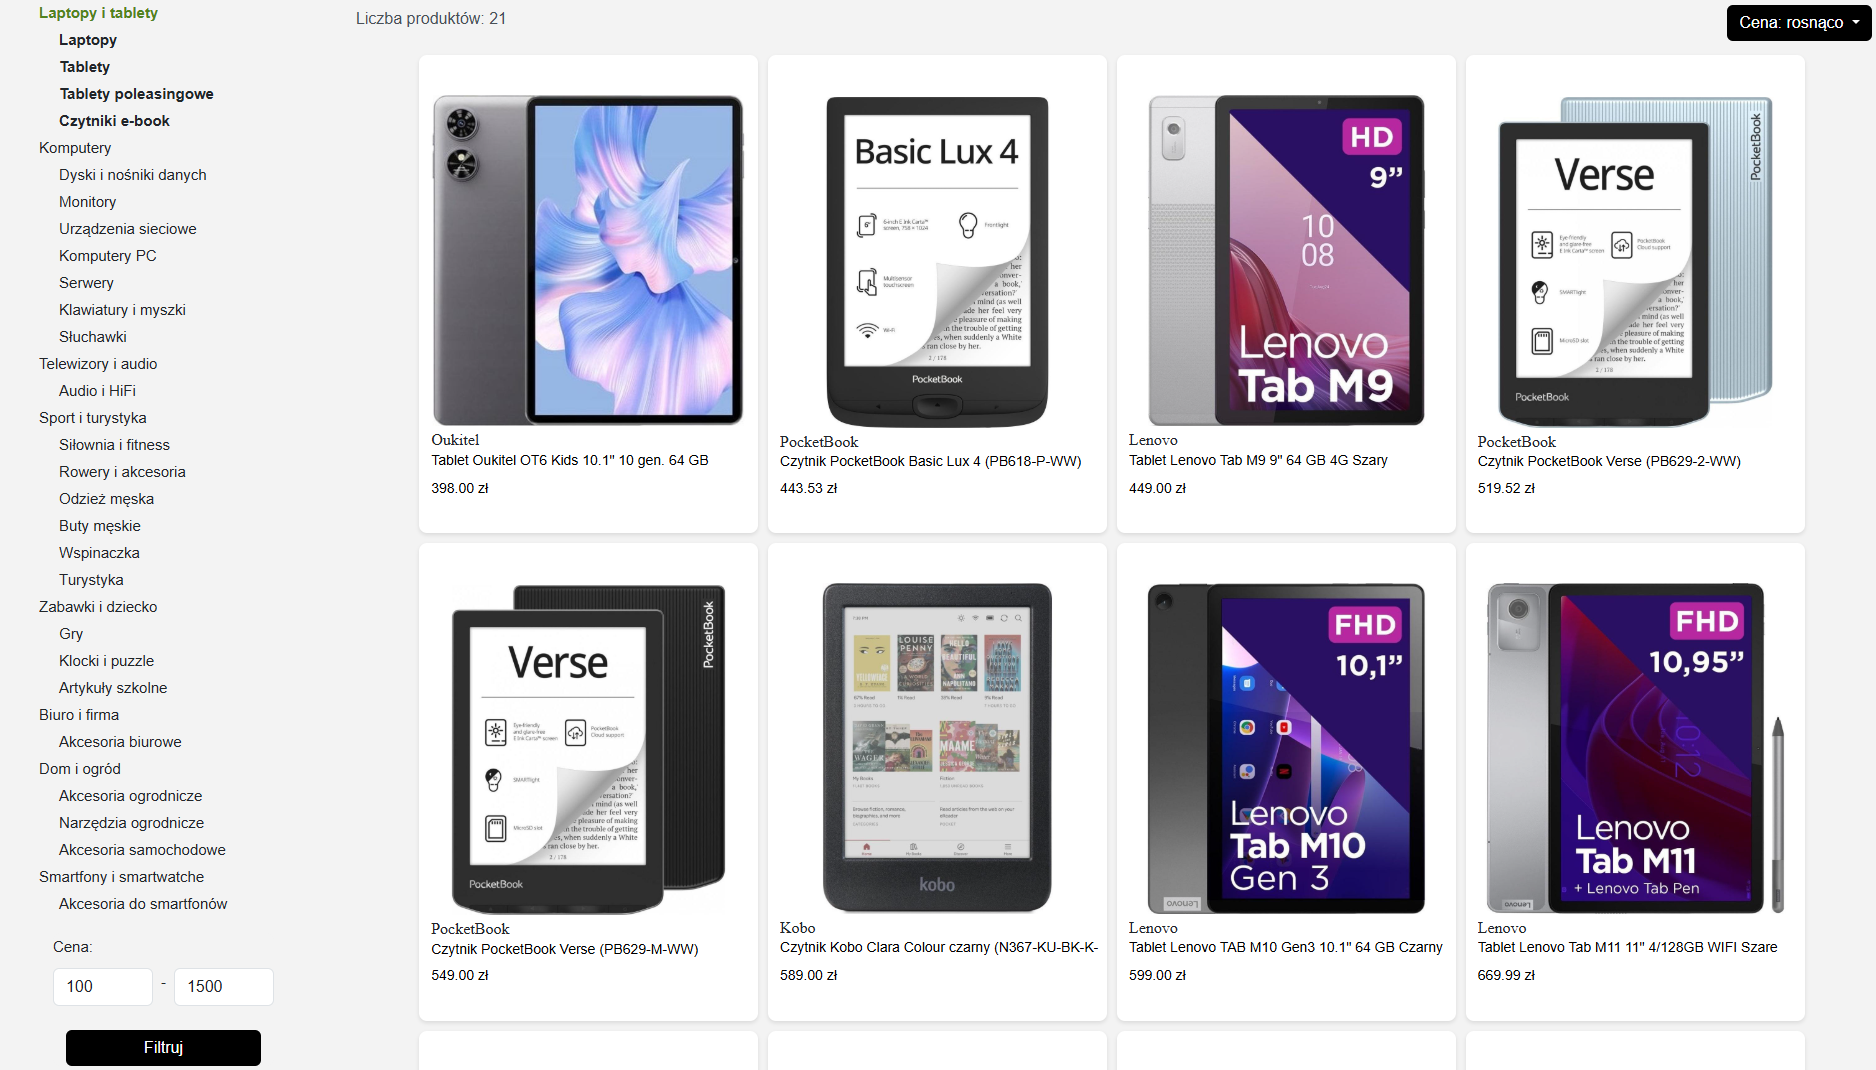
\includegraphics[width=1.0\columnwidth]{screens/order_filter.png}
    \caption{Widok filtrowania i sortowania produktów. \emph{Źródło: opracowanie własne.}}
    \label{fig:order_filter}
\end{figure}

\paragraph{Przykład działania}
1. Użytkownik wybiera kategorię produktów.
2. Korzystając z pól filtrowania, ustawia minimalną i maksymalną cenę i klika „Zastosuj”.
3. Produkty są wyświetlane zgodnie z ustawionym przedziałem cenowym.
4. Użytkownik wybiera kryterium sortowania (np. „Popularność”), a lista produktów zostaje uporządkowana zgodnie z wybranym kryterium.





\newpage
\subsection{Przykładowe działanie systemu}
\textit{Sekcja powinna zawierać tutoriale pokazujące realizację kluczowych funkcjonalności systemu dla przykładowych danych wejściowych.}



\subsubsection{Zakup produktu z rejestracją w systemie.}
Poniżej przedstawiono tutorial realizacji zakupu produktu krok po kroku, z uwzględnieniem kluczowych funkcjonalności systemu.

\subsubsection*{\textbf{1. Strona główna}}
Użytkownik rozpoczyna od strony głównej sklepu internetowego. Na górnym pasku dostępne są przyciski umożliwiające rejestrację i logowanie.

\begin{figure}[H]
    \centering
    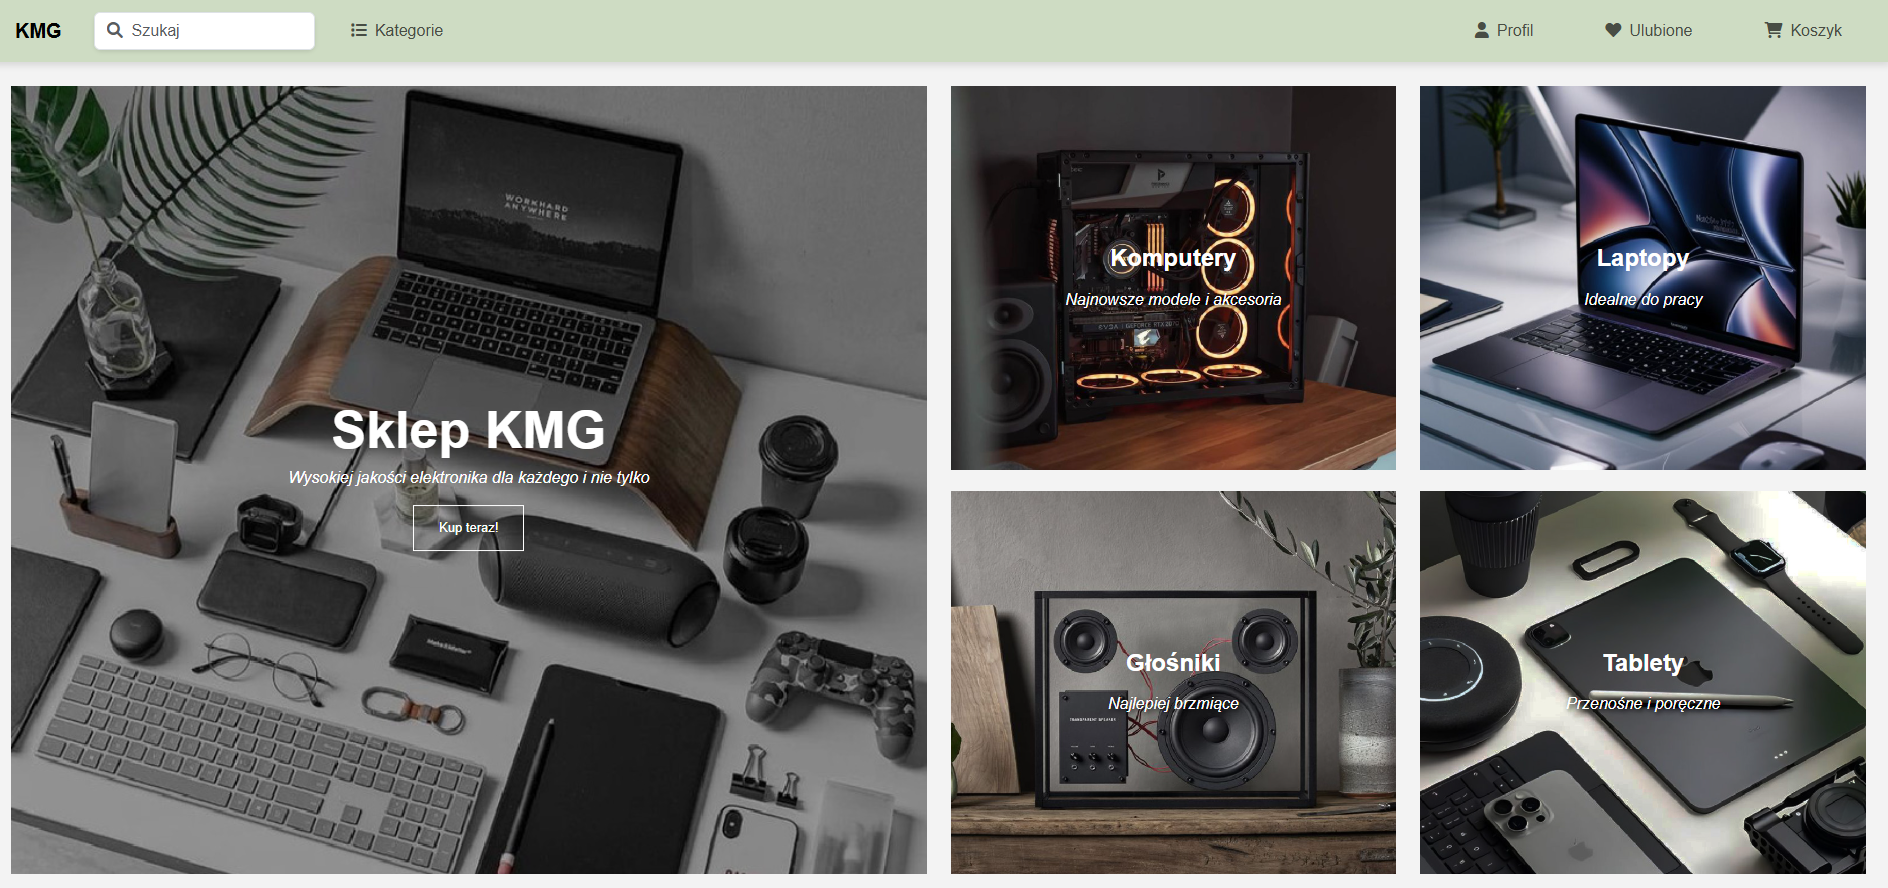
\includegraphics[width=1.0\columnwidth]{screens/main_page_tutorial.png}
    \caption{Strona główna sklepu internetowego. \emph{Źródło: opracowanie własne.}}
    \label{fig:main_page_tutorial}
\end{figure}

\subsubsection*{\textbf{2. Rejestracja}}
Użytkownik klika przycisk „Zarejestruj się” na górnym pasku. W formularzu rejestracyjnym wprowadza następujące dane:
\begin{itemize}
    \item Imię: \texttt{Maria},
    \item Nazwisko: \texttt{Nowak},
    \item Adres e-mail: \texttt{example@mail.com},
    \item Numer telefonu: \texttt{858654258},
    \item Data urodzenia: \texttt{12.04.1980},
    \item Płeć: \texttt{Kobieta},
    \item Hasło: \texttt{BezpieczneHaslo123},
\end{itemize}

\begin{figure}[H]
    \centering
    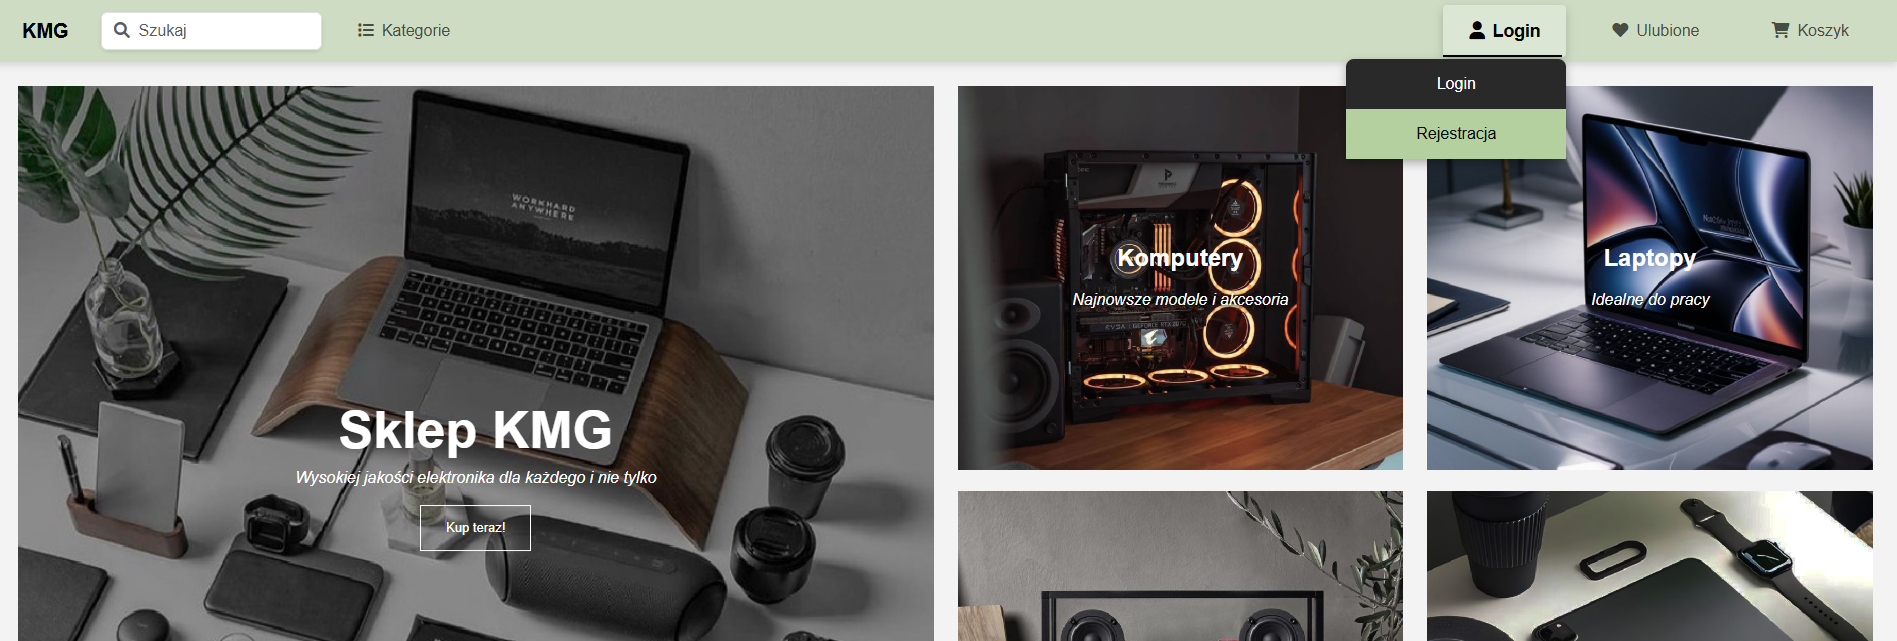
\includegraphics[width=1.0\columnwidth]{screens/register_btn_tutorial.png}
    \caption{Przycisk rejestracji na stronie głównej \emph{Źródło: opracowanie własne.}}
    \label{fig:register_btn_tutorial}
\end{figure}

\begin{figure}[H]
    \centering
    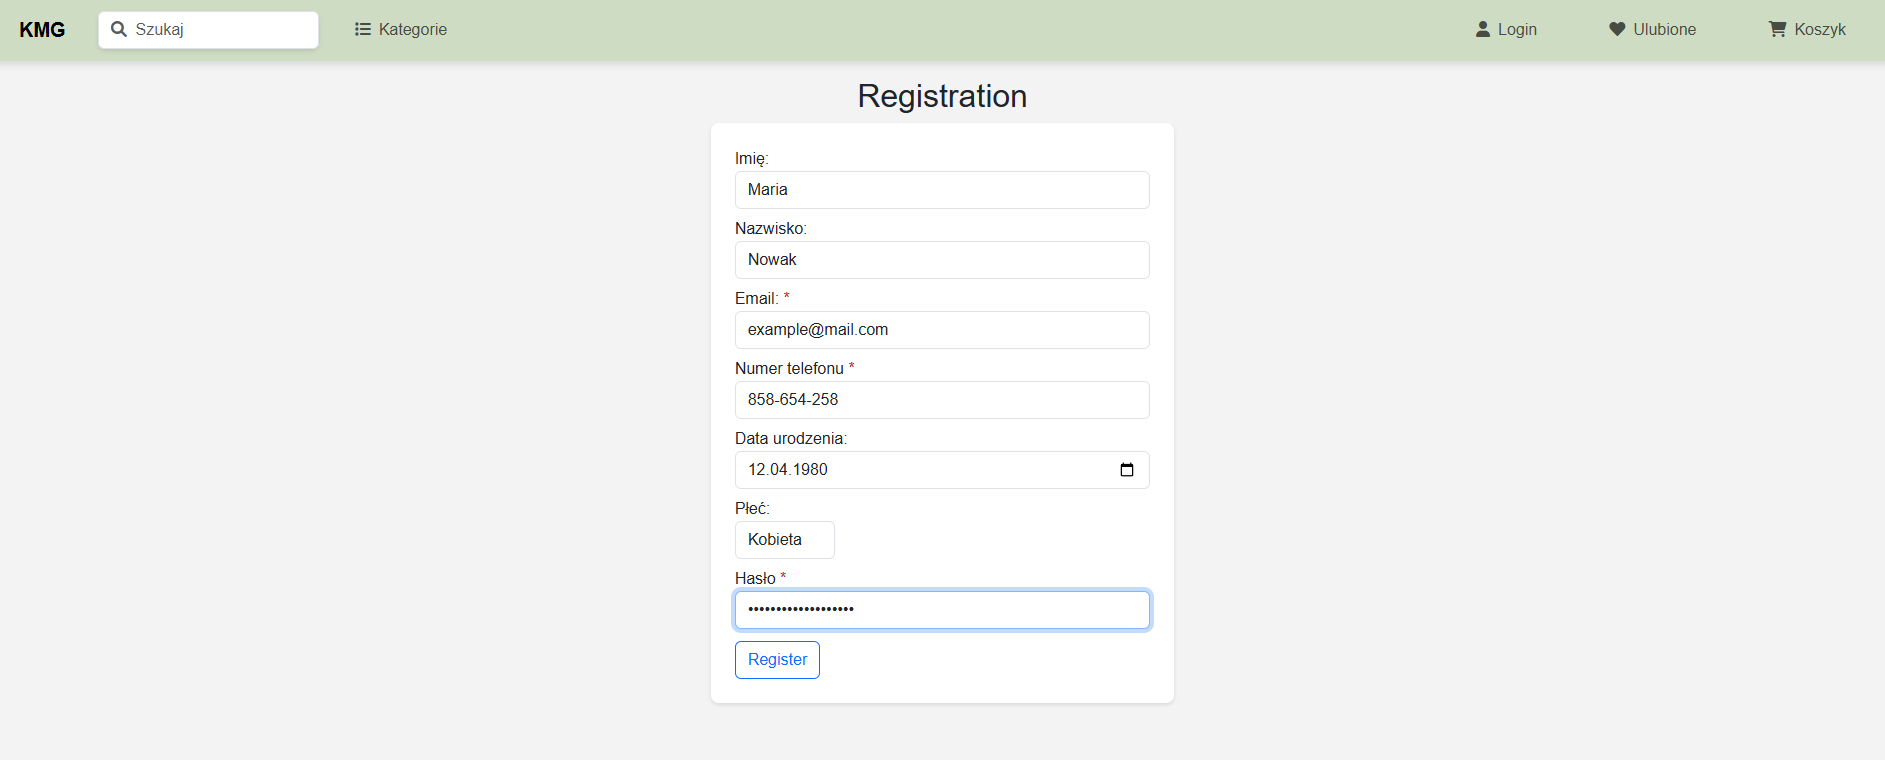
\includegraphics[width=1.0\columnwidth]{screens/register_form_tutorial.png}
    \caption{Uzupełniony formularz rejestracji \emph{Źródło: opracowanie własne.}}
    \label{fig:register_form_tutorial}
\end{figure}

\subsubsection*{\textbf{3. Logowanie}}
Po rejestracji użytkownik klika „Zaloguj się” i wprowadza swoje dane:
\begin{itemize}
    \item Adres e-mail: \texttt{example@mail.com},
    \item Hasło: \texttt{BezpieczneHaslo123}.
\end{itemize}
Kliknięcie „Zaloguj się” przenosi użytkownika na stronę główną z aktywnym profilem.

\begin{figure}[H]
    \centering
    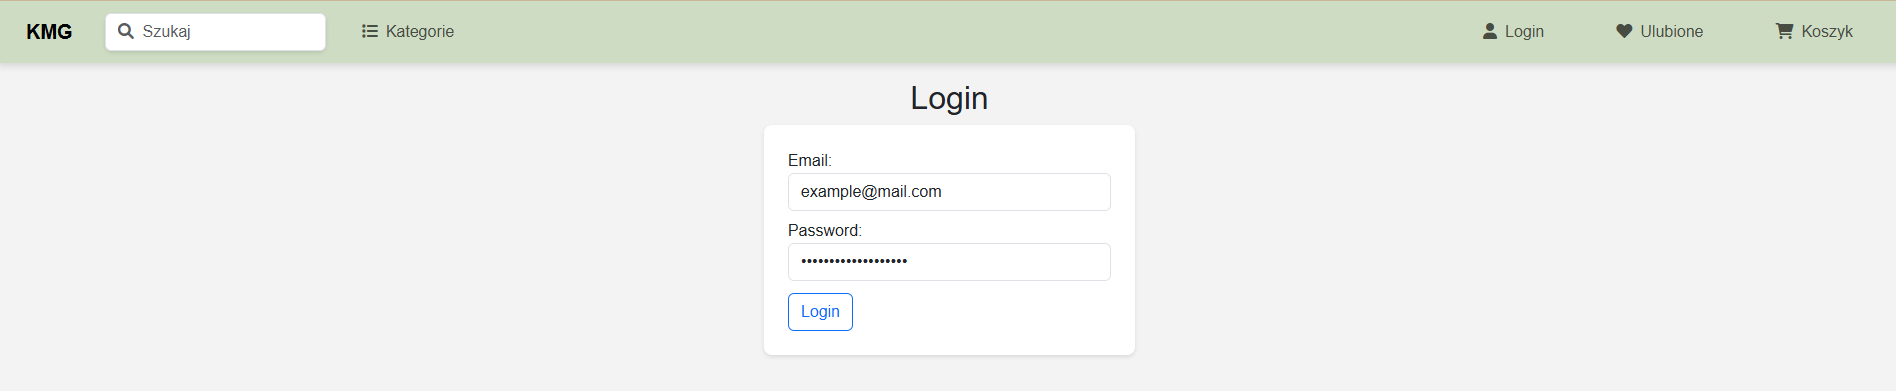
\includegraphics[width=1.0\columnwidth]{screens/login_tutorial.png}
    \caption{Formularz logowania \emph{Źródło: opracowanie własne.}}
    \label{fig:login_tutorial}
\end{figure}

\subsubsection*{\textbf{4. Wyszukiwanie produktu}}
Użytkownik wpisuje nazwę produktu \texttt{„Słuchawki JBL T770NC BT”} w pole wyszukiwania i naciska klawisz Enter. Wyświetla się lista wyników, w której użytkownik odnajduje interesujący go produkt.

\begin{figure}[H]
    \centering
    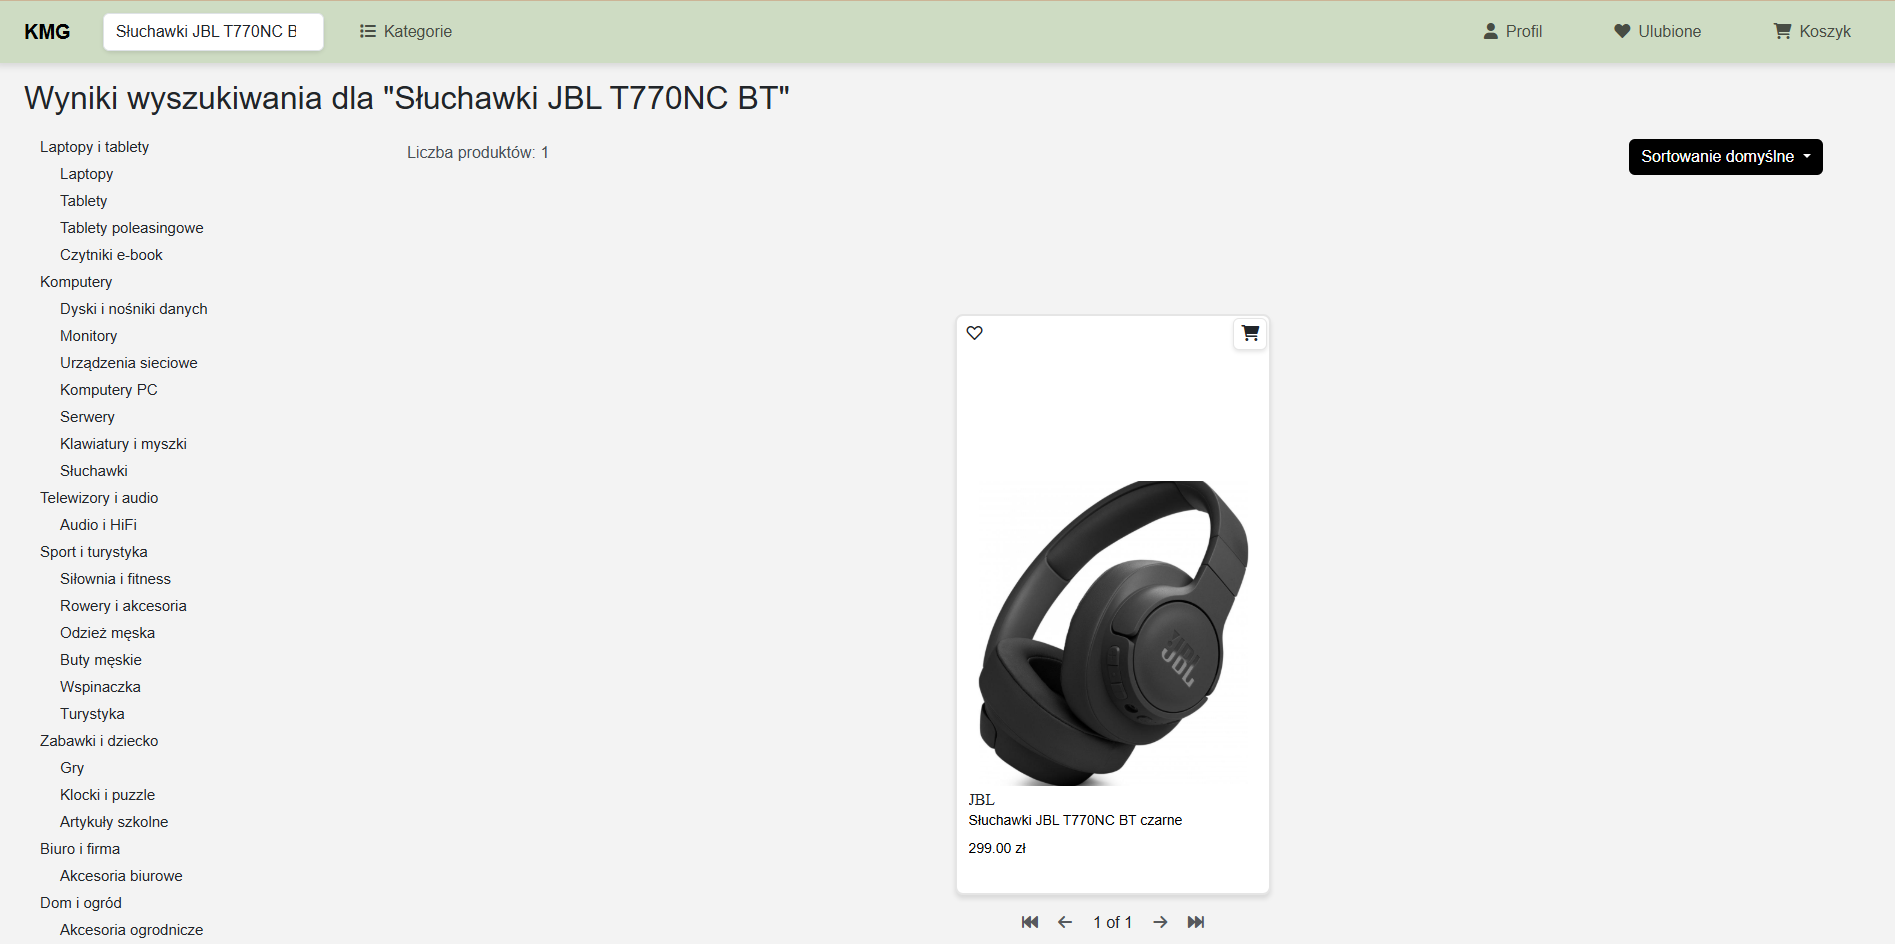
\includegraphics[width=1.0\columnwidth]{screens/search_result_tutorial.png}
    \caption{Wyniki wyszukiwania dla produktu „Słuchawki JBL T770NC BT”. \emph{Źródło: opracowanie własne.}}
    \label{fig:search_results_tutorial}
\end{figure}

\subsubsection*{\textbf{5. Dodanie produktu do koszyka}}
Użytkownik klika produkt, aby przejść do widoku szczegółowego, a następnie wybiera ilość (domyślnie 1) i klika przycisk „Dodaj do koszyka”. Na ekranie pojawia się potwierdzenie, że produkt został dodany.

\begin{figure}[H]
    \centering
    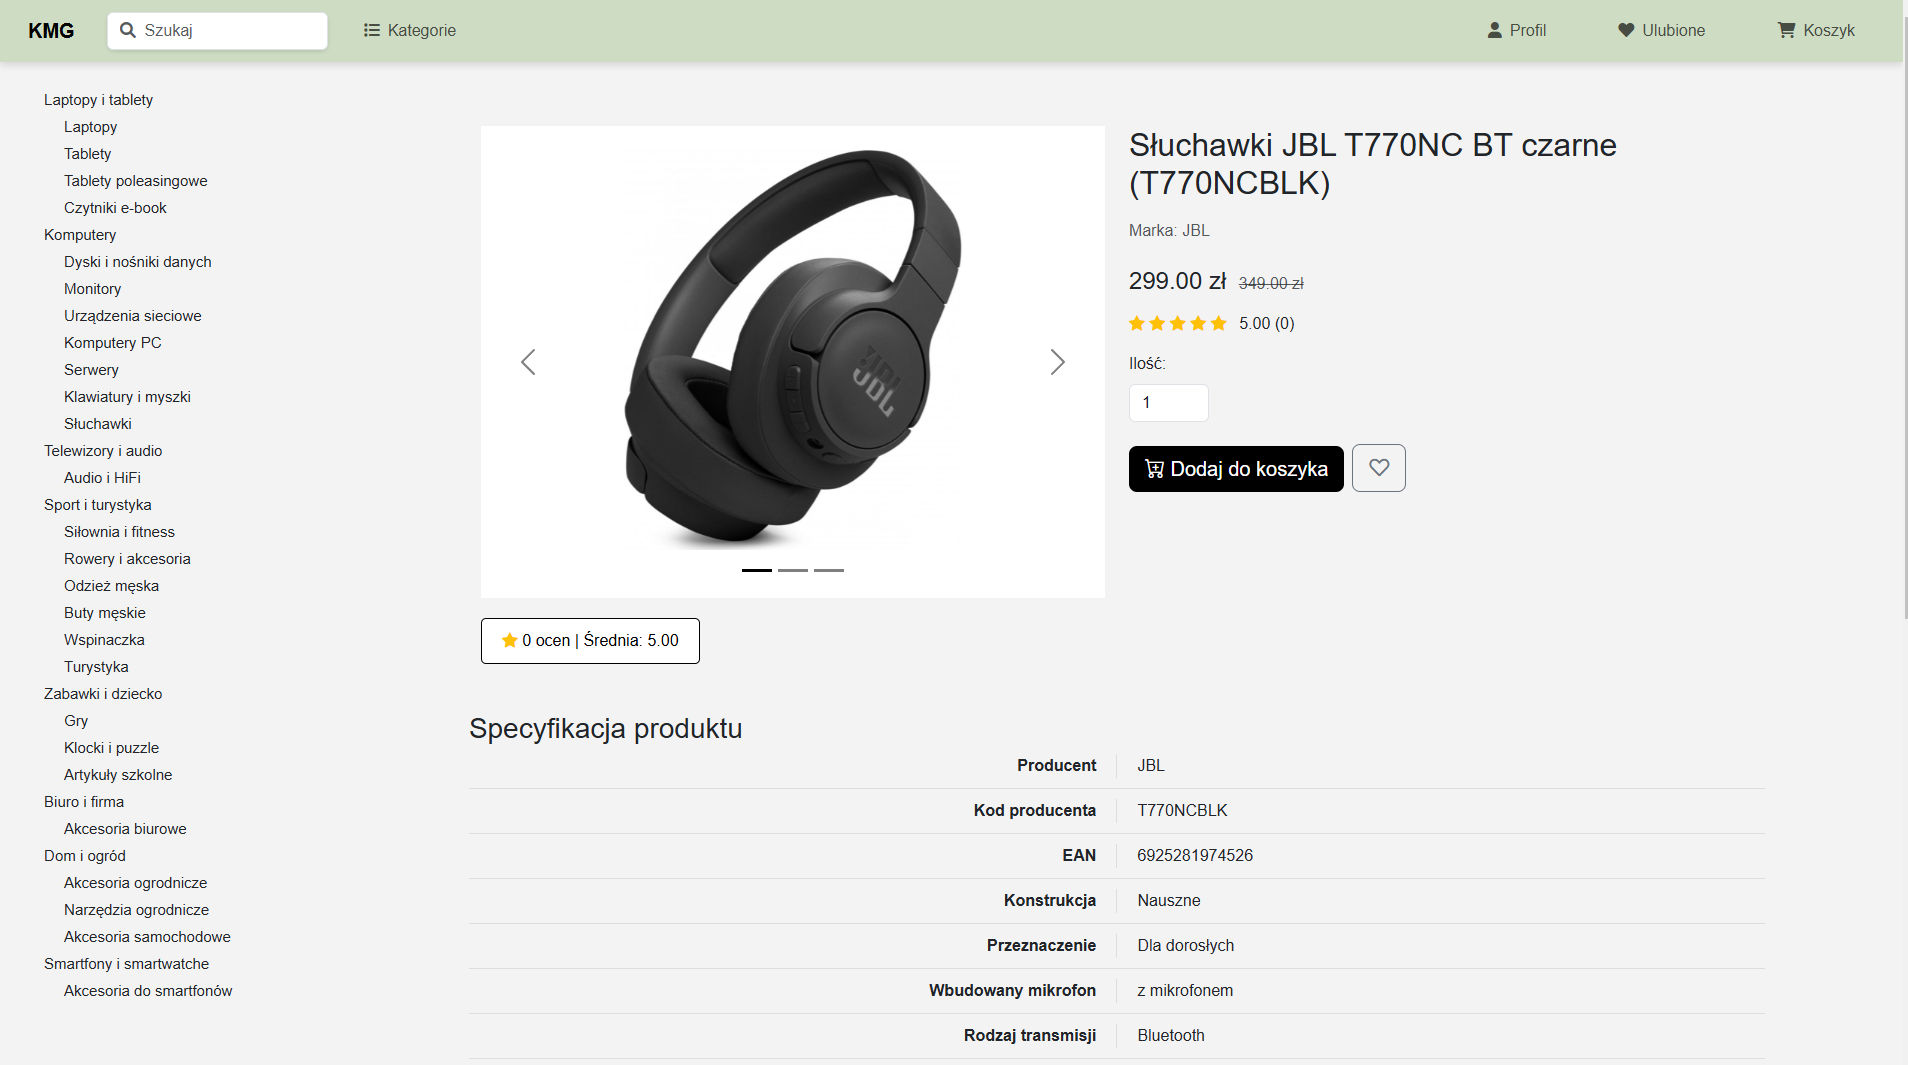
\includegraphics[width=1.0\columnwidth]{screens/product_details_tutorial.png}
    \caption{Szczegóły produktu „Słuchawki JBL T770NC BT” z opcją dodania do koszyka. \emph{Źródło: opracowanie własne.}}
    \label{fig:product_details_tutorial}
\end{figure}

\subsubsection*{\textbf{6. Zakup produktu}}
Użytkownik przechodzi do widoku koszyka i klika „Przejdź do opcji dostawy”. 
\begin{figure}[H]
    \centering
    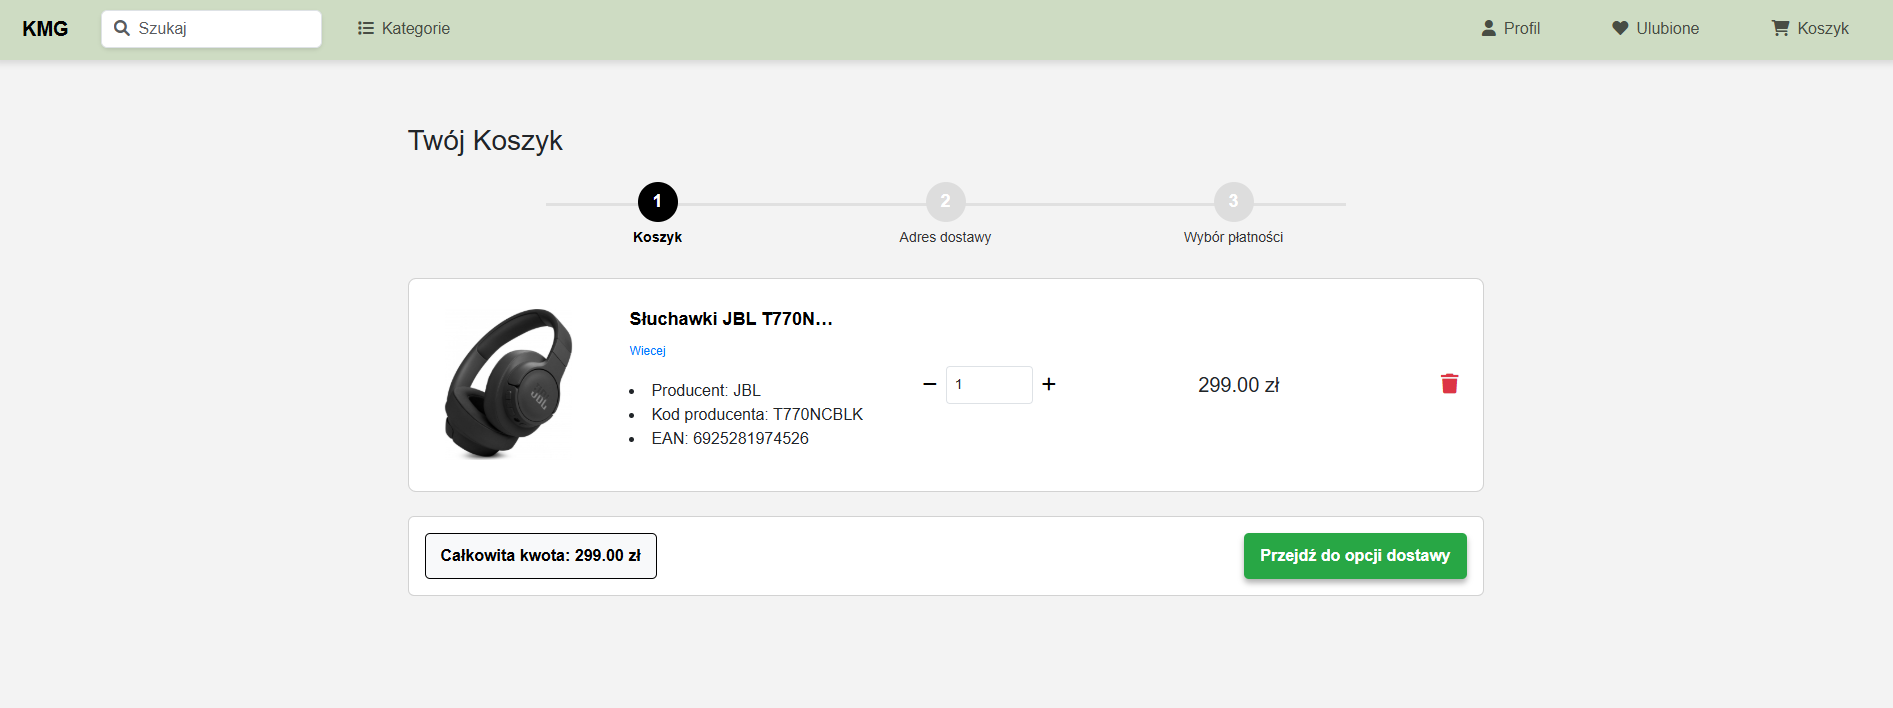
\includegraphics[width=1.0\columnwidth]{screens/order_details_tutorial.png}
    \caption{Koszyk z przyciskiem przejdź do do opcji dostawy. \emph{Źródło: opracowanie własne.}}
    \label{fig:order_details_first_tutorial}
\end{figure}
W sekcji wyboru adresu użytkownik wybiera lub dodaje adres:
\begin{itemize}
    \item Ulica: Krzemionki 6/23,
    \item Miasto: Kraków,
    \item Kod pocztowy: 30-069,
    \item Kraj: Polska.
\end{itemize}
\begin{figure}[H]
    \centering
    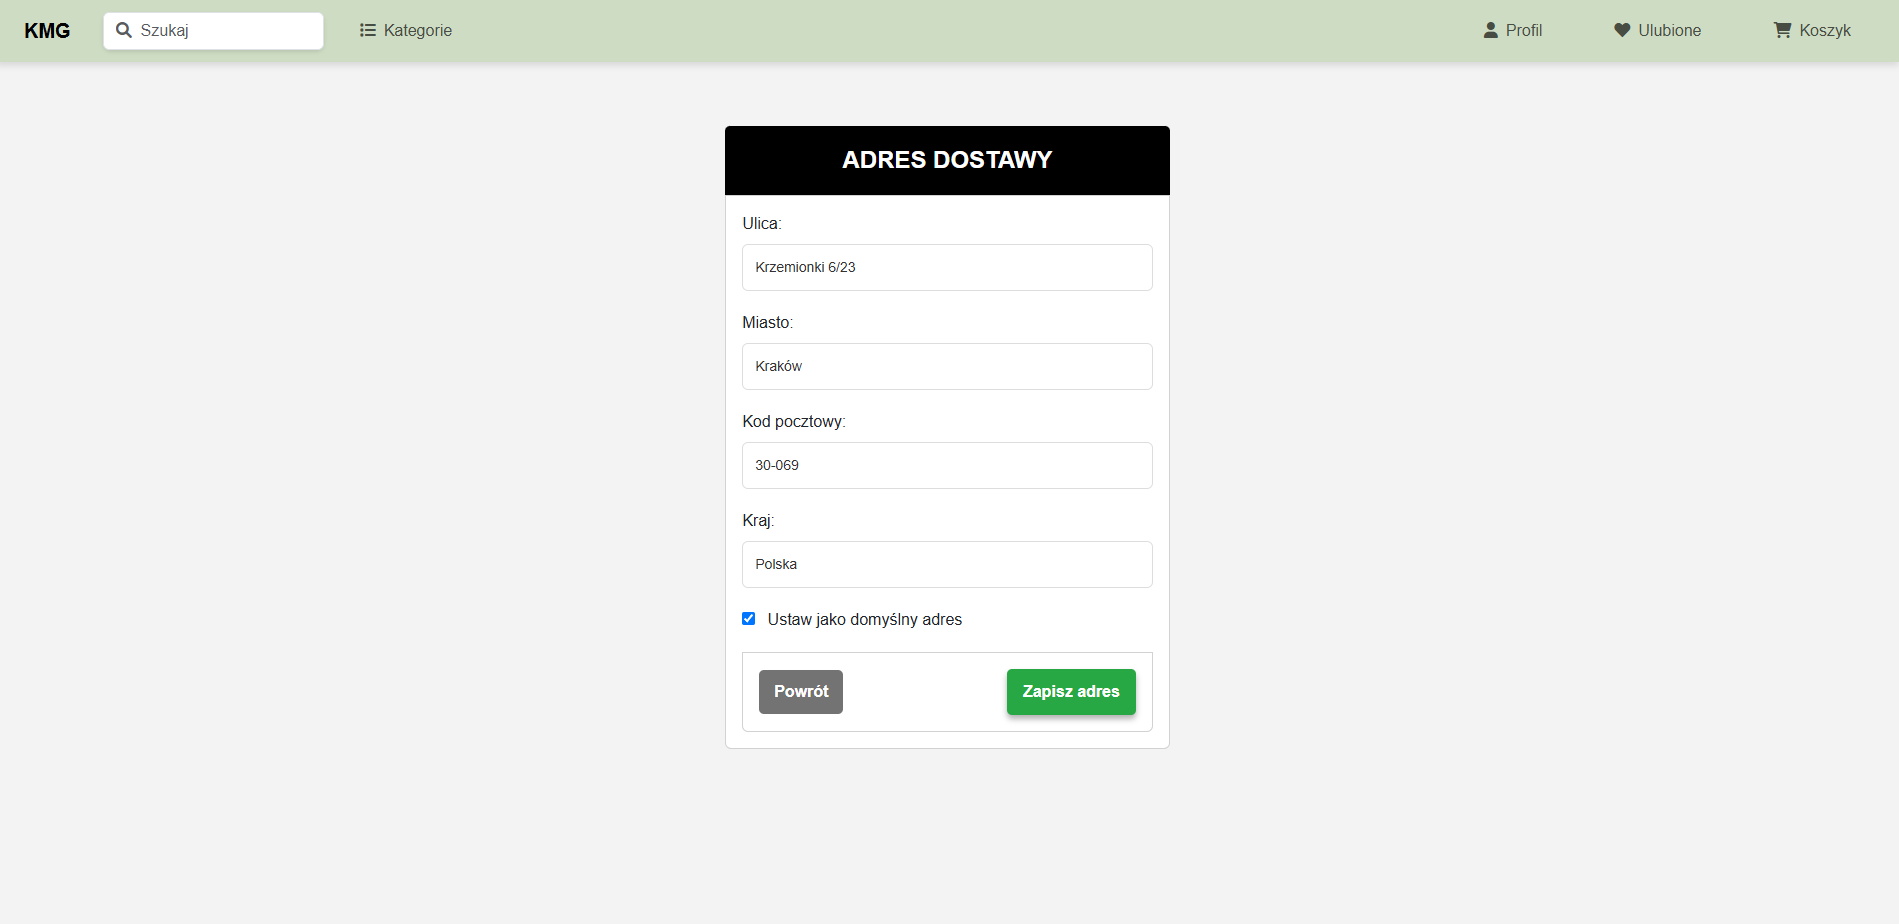
\includegraphics[width=1.0\columnwidth]{screens/add_address_tutorial.png}
    \caption{Dodanie adresu dostawy do pierwszego zamówienia. \emph{Źródło: opracowanie własne.}}
    \label{fig:add_address_tutorial}
\end{figure}


Następnie użytkownik klika „Przejdź do płatności” i wybiera metodę „Płatność za pobraniem”. Po zatwierdzeniu płatności użytkownik zostaje przekierowany do szczegółów zamówienia.

\begin{figure}[H]
    \centering
    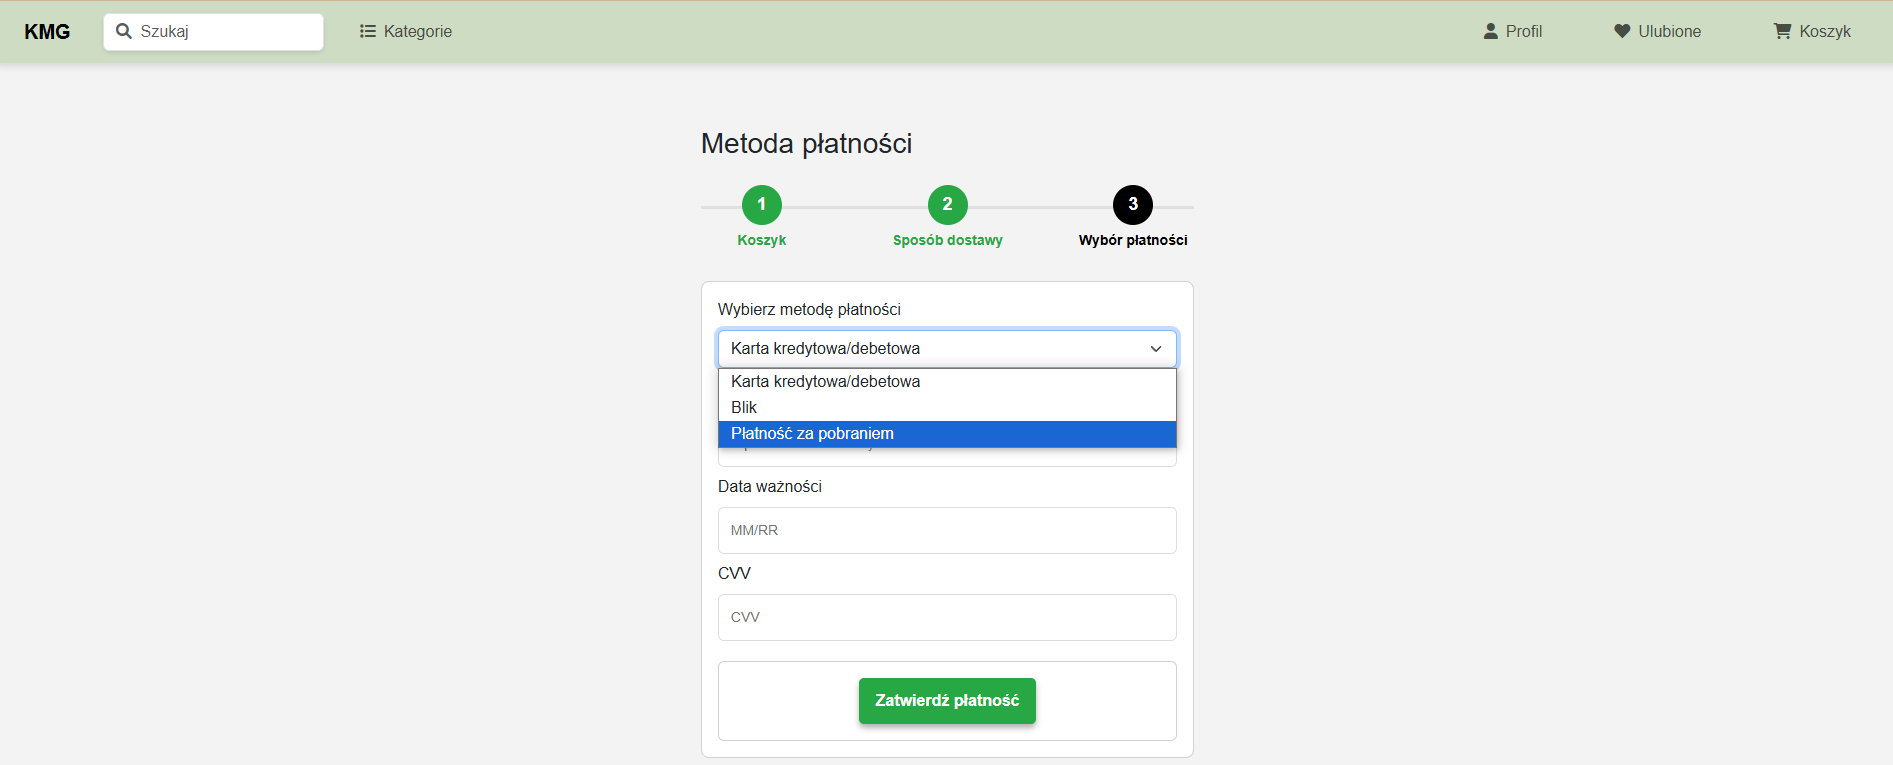
\includegraphics[width=1.0\columnwidth]{screens/payment_select_tutorial.png}
    \caption{Widok szczegółów zamówienia. \emph{Źródło: opracowanie własne.}}
    \label{fig:order_details_tutorial}
\end{figure}

\subsubsection*{\textbf{7. Finalizacja zamówienia}}
W szczegółach zamówienia użytkownik może zobaczyć podsumowanie:
\begin{itemize}
    \item ID zamówienia,
    \item Data zamówienia,
    \item Adres dostawy: Krzemionki 6/23, Kraków, 30-069, Polska,
    \item Metoda płatności: Płatność za pobraniem,
    \item Lista zamówionych produktów: „Słuchawki JBL T770NC BT” (1 szt.),
    \item Całkowita kwota zamówienia.
\end{itemize}
Na dole widoku widoczny jest pasek postępu zamówienia z aktualnym statusem „Utworzono”.

\begin{figure}[H]
    \centering
    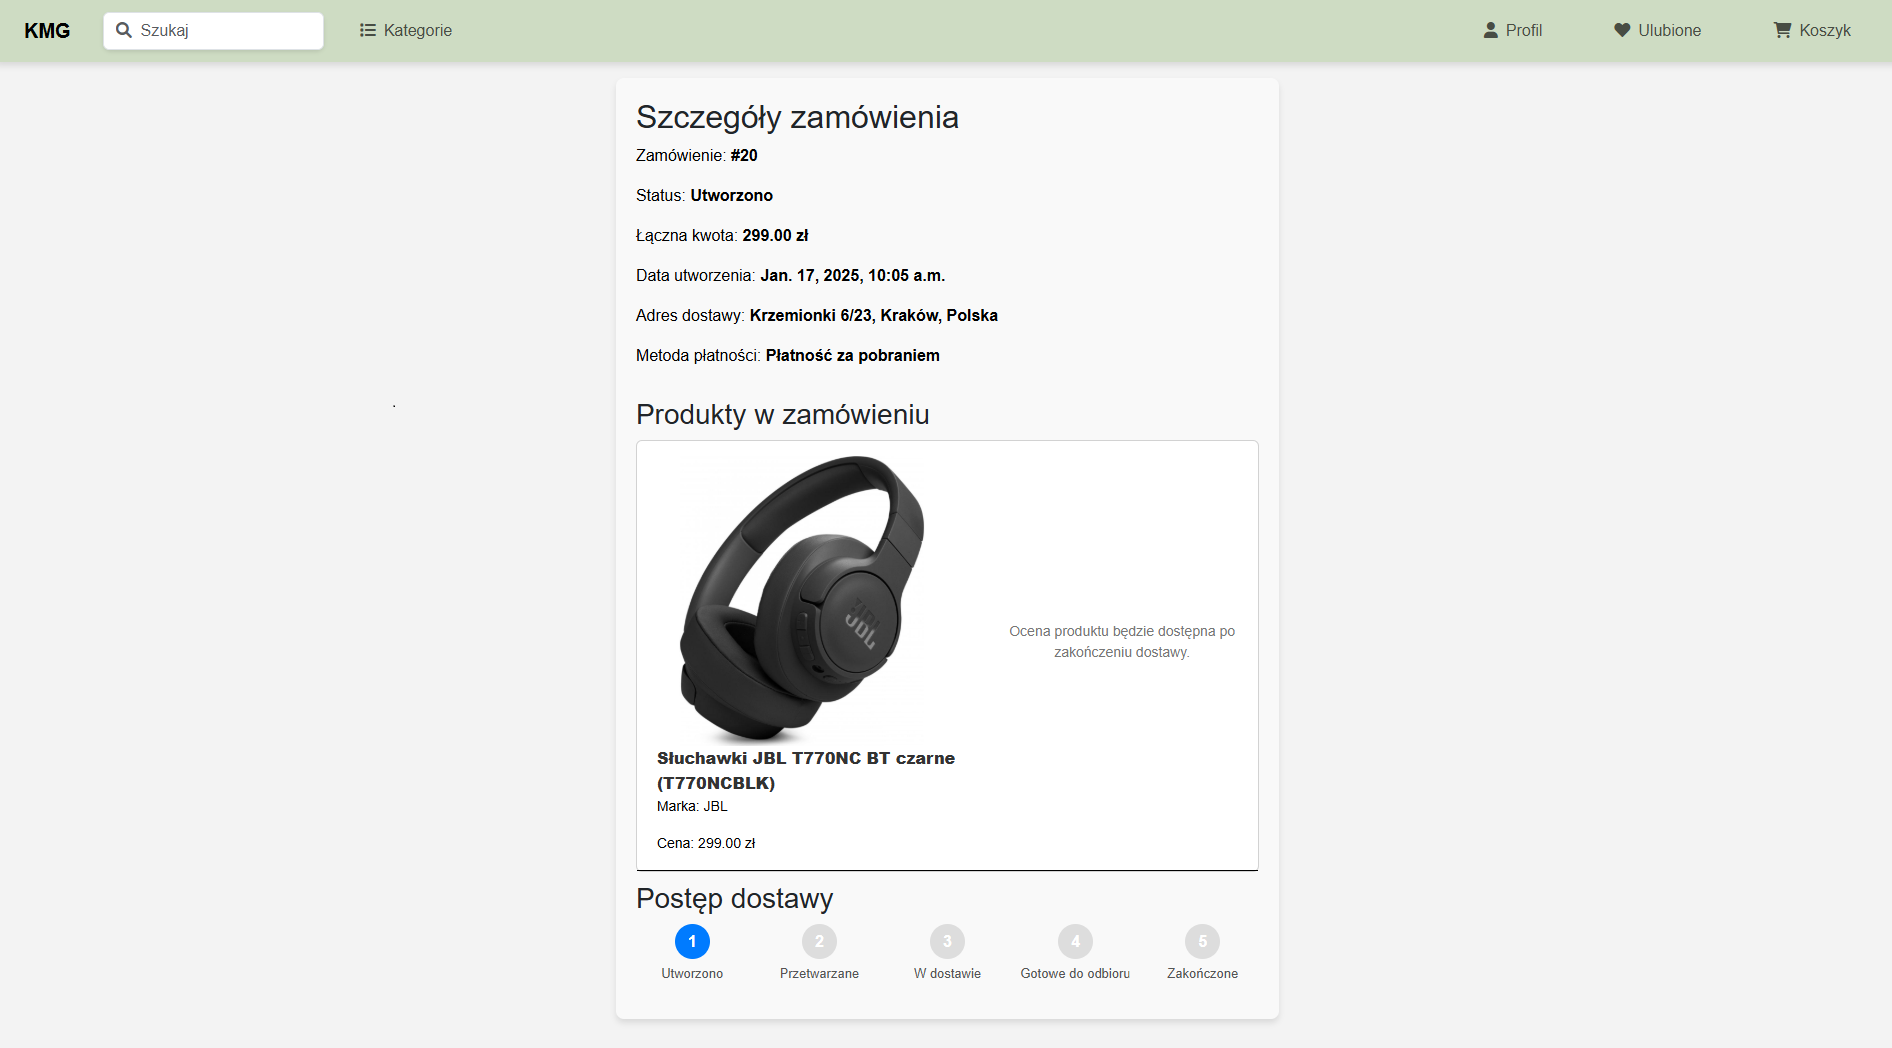
\includegraphics[width=1.0\columnwidth]{screens/order_status_create_tutorial.png}
    \caption{Pasek postępu zamówienia - zamówienie utworzone. \emph{Źródło: opracowanie własne.}}
    \label{fig:order_status_create_tutorial}
\end{figure}
\newpage
Po realizacji zamówienia status zmieni się na "Zakończone"

\begin{figure}[H]
    \centering
    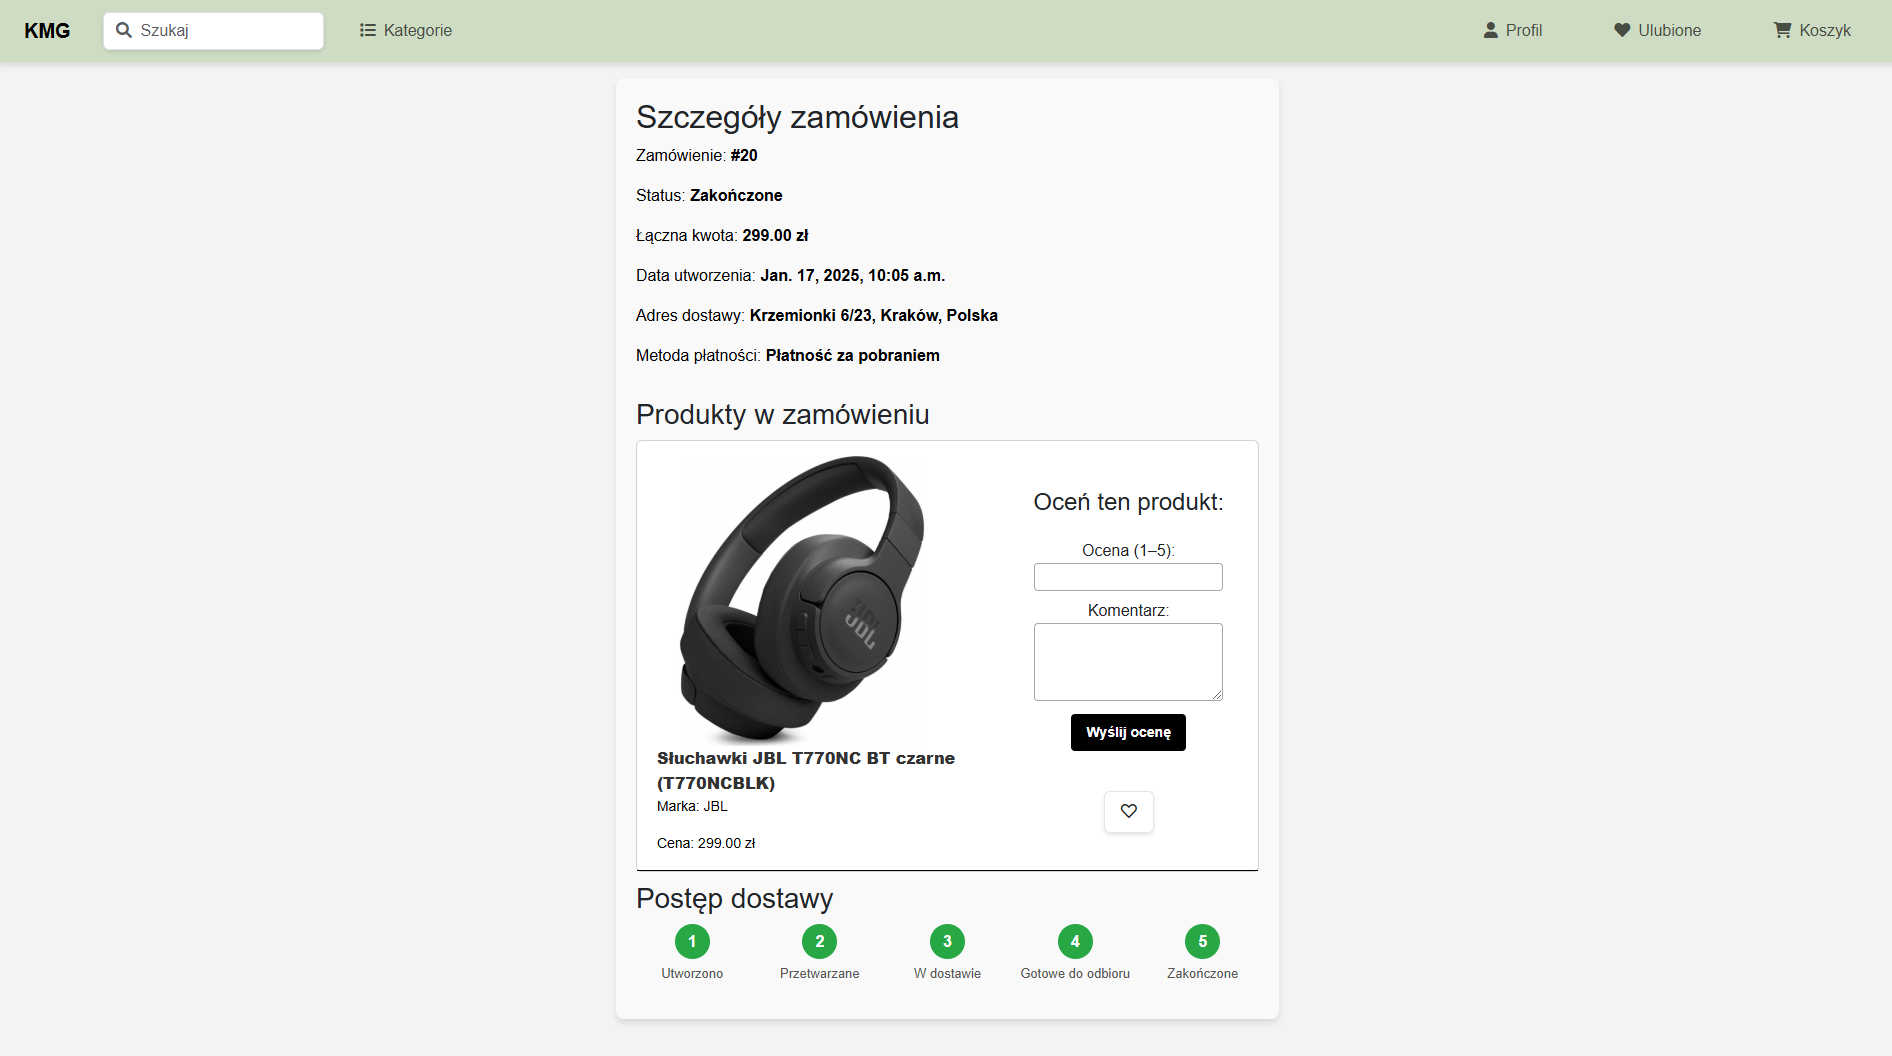
\includegraphics[width=1.0\columnwidth]{screens/order_status_tutorial.png}
    \caption{Pasek postępu zamówienia - zamówienie zrealizowane. \emph{Źródło: opracowanie własne.}}
    \label{fig:order_status_tutorial}
\end{figure}


\subsubsection{Przykład: Zmiana hasła użytkownika}
Poniżej przedstawiono krok po kroku proces zmiany hasła użytkownika z poziomu widoku „Profil”.

\subsubsection*{\textbf{1. Przejście do widoku Profil}}
Użytkownik klika przycisk „Profil” w górnym pasku nawigacyjnym. Zostaje przeniesiony do widoku profilu, gdzie znajdują się sekcje danych osobowych, w tym opcja zmiany hasła.

\begin{figure}[H]
    \centering
    
\includegraphics[width=1.0\columnwidth]{screens/profile_view.png}
    \caption{Widok Profil z sekcjami danych użytkownika. \emph{Źródło: opracowanie własne.}}
    \label{fig:profile_view_tutorial}
\end{figure}

\subsubsection*{\textbf{2. Rozpoczęcie procesu zmiany hasła}}
W sekcji „Zmiana hasła” użytkownik klika przycisk "Zmień hasło". Wyświetlają się pola umożliwiające wprowadzenie danych potrzebnych do zmiany hasła:
\begin{itemize}
    \item Aktualne hasło – weryfikacja tożsamości użytkownika,
    \item Nowe hasło – musi spełniać wymagania bezpieczeństwa (np. minimalna długość, użycie dużych i małych liter oraz cyfr),
    \item Potwierdzenie nowego hasła – weryfikacja poprawności wprowadzenia.
\end{itemize}

\begin{figure}[H]
    \centering
    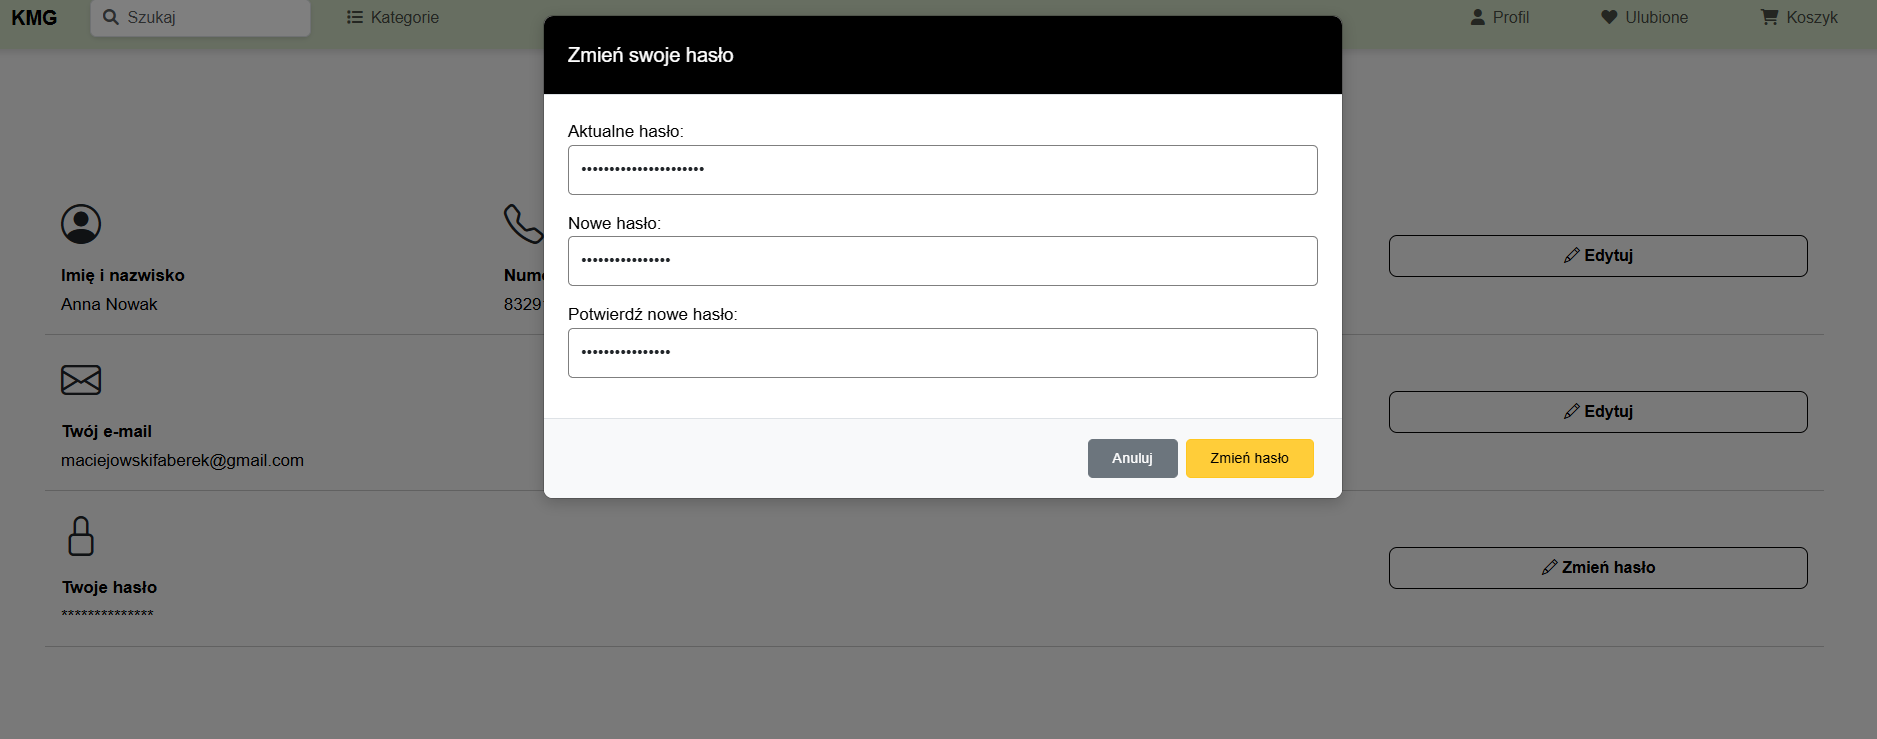
\includegraphics[width=1.0\columnwidth]{screens/password_change_form.png}
    \caption{Formularz zmiany hasła w widoku Profil. \emph{Źródło: opracowanie własne.}}
    \label{fig:password_change_form}
\end{figure}

\subsubsection*{\textbf{3. Zatwierdzenie zmian}}
Po wypełnieniu pól użytkownik klika przycisk „Zapisz zmiany”. System wykonuje następujące kroki:
\begin{itemize}
    \item Weryfikuje, czy aktualne hasło jest poprawne,
    \item Sprawdza, czy nowe hasło spełnia wymagania bezpieczeństwa,
    \item Porównuje nowe hasło z jego potwierdzeniem.
\end{itemize}

\paragraph{Wynik procesu zmiany hasła:}
\begin{itemize}
    \item Jeśli wszystkie dane są poprawne, zmiana hasła zostaje zatwierdzona, a użytkownik otrzymuje komunikat: „Hasło zostało zmienione".
    \item Jeśli wystąpi błąd (np. błędne aktualne hasło lub niespełnienie wymagań bezpieczeństwa), użytkownik otrzymuje odpowiedni komunikat i może ponowić próbę.
\end{itemize}

\subsubsection*{\textbf{4. Zakończenie procesu}}
Po pomyślnej zmianie hasła użytkownik może kontynuować korzystanie z systemu. W przypadku wylogowania musi zalogować się, używając nowego hasła.

\begin{figure}[H]
    \centering
    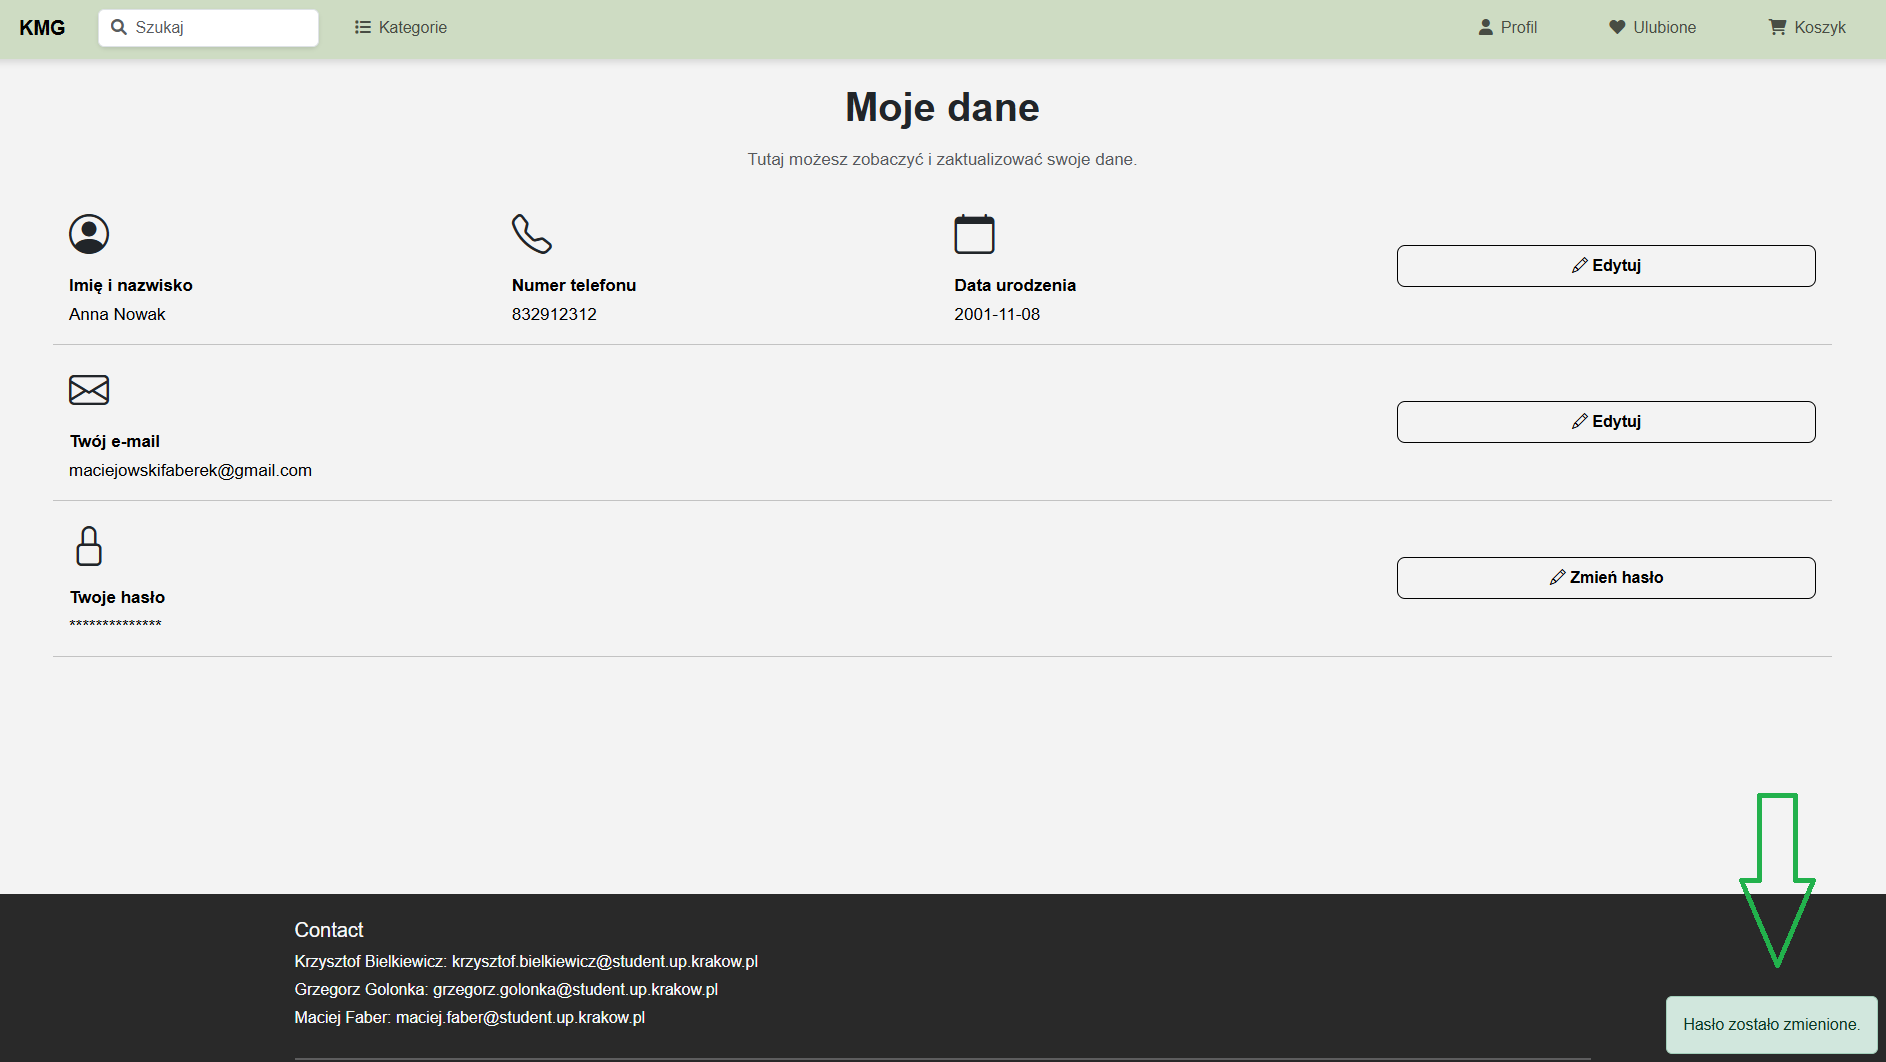
\includegraphics[width=1.0\columnwidth]{screens/password_change_success.png}
    \caption{Komunikat o pomyślnej zmianie hasła. \emph{Źródło: opracowanie własne.}}
    \label{fig:password_change_success}
\end{figure}

\newpage
\addcontentsline{toc}{section}{Lista rysunków}
\listoffigures
%\bibliography{references}
% --------------------------------------------------------------------
%%%%%%% odkomentować gdy bibliografia ma być wewnątrz dokumentu
% --------------------------------------------------------------------
%\begin{thebibliography}{11}
%
%\addcontentsline{toc}{section}{Literatura}
%
%\bibitem{ZAN}
%C. Zannoni and P. Pasini, 
%\emph{Advances in the Computer Simulatons of Liquid Crystals}, Kluwer Academic Publishers, 2000.
%
%\end{thebibliography}

\end{document}

